% Plantilla para un Trabajo Fin de Grado de la Universidad de Granada,
% adaptada para el Doble Grado en Ingeniería Informática y Matemáticas.
%
%  Autor: Mario Román.
%  Licencia: GNU GPLv2.
%
% Esta plantilla es una adaptación al castellano de la plantilla
% classicthesis de André Miede, que puede obtenerse en:
%  https://ctan.org/tex-archive/macros/latex/contrib/classicthesis?lang=en
% La plantilla original se licencia en GNU GPLv2.
%
% Esta plantilla usa símbolos de la Universidad de Granada sujetos a la normativa
% de identidad visual corporativa, que puede encontrarse en:
% http://secretariageneral.ugr.es/pages/ivc/normativa
%
% La compilación se realiza con las siguientes instrucciones:
%   pdflatex --shell-escape main.tex
%   bibtex main
%   pdflatex --shell-escape main.tex
%   pdflatex --shell-escape main.tex

% Opciones del tipo de documento
\documentclass[oneside,openright,titlepage,numbers=noenddot,headinclude,footinclude=true,
cleardoublepage=empty,abstractoff,BCOR=5mm,paper=a4,fontsize=12pt,main=spanish]{scrreprt}

% Paquetes de latex que se cargan al inicio. Cubren la entrada de
% texto, gráficos, código fuente y símbolos.
\usepackage[utf8]{inputenc}
\usepackage[T1]{fontenc}
\usepackage{fixltx2e}
\usepackage{graphicx} % Inclusión de imágenes.
\usepackage{grffile}  % Distintos formatos para imágenes.
\usepackage{longtable} % Tablas multipágina.
\usepackage{wrapfig} % Coloca texto alrededor de una figura.
\usepackage{rotating}
\usepackage[normalem]{ulem}
\usepackage{amsmath}
\usepackage{textcomp}
\usepackage{amssymb}
\usepackage{capt-of}
\usepackage[colorlinks=true]{hyperref}
\usepackage{tikz} % Diagramas conmutativos.
\usepackage{minted} % Código fuente.
\usepackage[T1]{fontenc}
\usepackage{natbib}

% Plantilla classicthesis
\usepackage[beramono,eulerchapternumbers,linedheaders,parts,a5paper,dottedtoc,
manychapters,pdfspacing]{classicthesis}

% Geometría y espaciado de párrafos.
\setcounter{secnumdepth}{0}
\usepackage{enumitem}
\setitemize{noitemsep,topsep=0pt,parsep=0pt,partopsep=0pt}
\setlist[enumerate]{topsep=0pt,itemsep=-1ex,partopsep=1ex,parsep=1ex}
\usepackage[top=1in, bottom=1.5in, left=1in, right=1in]{geometry}
\setlength\itemsep{0em}
\setlength{\parindent}{0pt}
\usepackage{parskip}

% Profundidad de la tabla de contenidos.
\setcounter{secnumdepth}{3}

% Usa el paquete minted para mostrar trozos de código.
% Pueden seleccionarse el lenguaje apropiado y el estilo del código.
\usepackage{minted}
\usemintedstyle{colorful}
\setminted{fontsize=\small}
\setminted[haskell]{linenos=false,fontsize=\small}
\renewcommand{\theFancyVerbLine}{\sffamily\textcolor[rgb]{0.5,0.5,1.0}
{\oldstylenums{\arabic{FancyVerbLine}}}}


% Archivos de configuración.
%------------------------
% Bibliotecas para matemáticas de latex
%------------------------
\usepackage{amsthm}
\usepackage{amsmath}
\usepackage{tikz}
\usepackage{tikz-cd}
\usetikzlibrary{shapes,fit}
\usepackage{bussproofs}
\EnableBpAbbreviations{}
\usepackage{mathtools}
\usepackage{scalerel}
\usepackage{stmaryrd}

%------------------------
% Estilos para los teoremas
%------------------------
\theoremstyle{plain}
\newtheorem{theorem}{Teorema}
\newtheorem{proposition}{Proposición}
\newtheorem{lemma}{Lema}
\newtheorem{corollary}{Corolario}
\theoremstyle{definition}
\newtheorem{definition}{Definición}
\newtheorem{proofs}{Demostración}
\theoremstyle{remark}
\newtheorem{remark}{Comentario}
\newtheorem{exampleth}{Ejemplo}

\begingroup\makeatletter\@for\theoremstyle:=definition,remark,plain\do{\expandafter\g@addto@macro\csname th@\theoremstyle\endcsname{\addtolength\thm@preskip\parskip}}\endgroup

%------------------------
% Macros
% ------------------------

% Aquí pueden añadirse abreviaturas para comandos de latex
% frequentemente usados.
\newcommand*\diff{\mathop{}\!\mathrm{d}}  % En macros.tex se almacenan las opciones y comandos para escribir matemáticas.
% ****************************************************************************************************
% classicthesis-config.tex 
% formerly known as loadpackages.sty, classicthesis-ldpkg.sty, and classicthesis-preamble.sty 
% Use it at the beginning of your ClassicThesis.tex, or as a LaTeX Preamble 
% in your ClassicThesis.{tex,lyx} with % ****************************************************************************************************
% classicthesis-config.tex 
% formerly known as loadpackages.sty, classicthesis-ldpkg.sty, and classicthesis-preamble.sty 
% Use it at the beginning of your ClassicThesis.tex, or as a LaTeX Preamble 
% in your ClassicThesis.{tex,lyx} with % ****************************************************************************************************
% classicthesis-config.tex 
% formerly known as loadpackages.sty, classicthesis-ldpkg.sty, and classicthesis-preamble.sty 
% Use it at the beginning of your ClassicThesis.tex, or as a LaTeX Preamble 
% in your ClassicThesis.{tex,lyx} with \input{classicthesis-config}
% ****************************************************************************************************  
% If you like the classicthesis, then I would appreciate a postcard. 
% My address can be found in the file ClassicThesis.pdf. A collection 
% of the postcards I received so far is available online at 
% http://postcards.miede.de
% ****************************************************************************************************


% ****************************************************************************************************
% 0. Set the encoding of your files. UTF-8 is the only sensible encoding nowadays. If you can't read
% äöüßáéçèê∂åëæƒÏ€ then change the encoding setting in your editor, not the line below. If your editor
% does not support utf8 use another editor!
% ****************************************************************************************************
\PassOptionsToPackage{utf8x}{inputenc}
	\usepackage{inputenc}

% ****************************************************************************************************
% 1. Configure classicthesis for your needs here, e.g., remove "drafting" below 
% in order to deactivate the time-stamp on the pages
% ****************************************************************************************************
\PassOptionsToPackage{eulerchapternumbers,listings,drafting,%
		pdfspacing,%floatperchapter,%linedheaders,%
                subfig,beramono,eulermath,parts,dottedtoc}{classicthesis}                                        
% ********************************************************************
% Available options for classicthesis.sty 
% (see ClassicThesis.pdf for more information):
% drafting
% parts nochapters linedheaders
% eulerchapternumbers beramono eulermath pdfspacing minionprospacing
% tocaligned dottedtoc manychapters
% listings floatperchapter subfig
% ********************************************************************

% ****************************************************************************************************
% 2. Personal data and user ad-hoc commands
% ****************************************************************************************************
\newcommand{\myTitle}{A Classic Thesis Style\xspace}
\newcommand{\mySubtitle}{An Homage to The Elements of Typographic Style\xspace}
\newcommand{\myDegree}{Doktor-Ingenieur (Dr.-Ing.)\xspace}
\newcommand{\myName}{André Miede\xspace}
\newcommand{\myProf}{Put name here\xspace}
\newcommand{\myOtherProf}{Put name here\xspace}
\newcommand{\mySupervisor}{Put name here\xspace}
\newcommand{\myFaculty}{Put data here\xspace}
\newcommand{\myDepartment}{Put data here\xspace}
\newcommand{\myUni}{Put data here\xspace}
\newcommand{\myLocation}{Saarbrücken\xspace}
\newcommand{\myTime}{September 2015\xspace}
%\newcommand{\myVersion}{version 4.2\xspace}

% ********************************************************************
% Setup, finetuning, and useful commands
% ********************************************************************
\newcounter{dummy} % necessary for correct hyperlinks (to index, bib, etc.)
\newlength{\abcd} % for ab..z string length calculation
\providecommand{\mLyX}{L\kern-.1667em\lower.25em\hbox{Y}\kern-.125emX\@}
\newcommand{\ie}{i.\,e.}
\newcommand{\Ie}{I.\,e.}
\newcommand{\eg}{e.\,g.}
\newcommand{\Eg}{E.\,g.} 
% ****************************************************************************************************


% ****************************************************************************************************
% 3. Loading some handy packages
% ****************************************************************************************************
% ******************************************************************** 
% Packages with options that might require adjustments
% ******************************************************************** 
%\PassOptionsToPackage{ngerman,american}{babel}   % change this to your language(s)
% Spanish languages need extra options in order to work with this template
% \PassOptionsToPackage{es-lcroman,spanish}{babel}
\usepackage[main=spanish]{babel}

%\usepackage{csquotes}
% \PassOptionsToPackage{%
%     %backend=biber, %instead of bibtex
% 	backend=bibtex8,bibencoding=ascii,%
% 	language=auto,%
% 	style=alpha,%
%     %style=authoryear-comp, % Author 1999, 2010
%     %bibstyle=authoryear,dashed=false, % dashed: substitute rep. author with ---
%     sorting=nyt, % name, year, title
%     maxbibnames=10, % default: 3, et al.
%     %backref=true,%
%     natbib=true % natbib compatibility mode (\citep and \citet still work)
% }{biblatex}
%     \usepackage{biblatex}

% \PassOptionsToPackage{fleqn}{amsmath}       % math environments and more by the AMS 
%     \usepackage{amsmath}

% ******************************************************************** 
% General useful packages
% ******************************************************************** 
\PassOptionsToPackage{T1}{fontenc} % T2A for cyrillics
    \usepackage{fontenc}     
\usepackage{textcomp} % fix warning with missing font shapes
\usepackage{scrhack} % fix warnings when using KOMA with listings package          
\usepackage{xspace} % to get the spacing after macros right  
\usepackage{mparhack} % get marginpar right
\usepackage{fixltx2e} % fixes some LaTeX stuff --> since 2015 in the LaTeX kernel (see below)
%\usepackage[latest]{latexrelease} % will be used once available in more distributions (ISSUE #107)
\PassOptionsToPackage{printonlyused,smaller}{acronym} 
    \usepackage{acronym} % nice macros for handling all acronyms in the thesis
    %\renewcommand{\bflabel}[1]{{#1}\hfill} % fix the list of acronyms --> no longer working
    %\renewcommand*{\acsfont}[1]{\textsc{#1}} 
    \renewcommand*{\aclabelfont}[1]{\acsfont{#1}}
% ****************************************************************************************************


% ****************************************************************************************************
% 4. Setup floats: tables, (sub)figures, and captions
% ****************************************************************************************************
\usepackage{tabularx} % better tables
    \setlength{\extrarowheight}{3pt} % increase table row height
\newcommand{\tableheadline}[1]{\multicolumn{1}{c}{\spacedlowsmallcaps{#1}}}
\newcommand{\myfloatalign}{\centering} % to be used with each float for alignment
\usepackage{caption}
% Thanks to cgnieder and Claus Lahiri
% http://tex.stackexchange.com/questions/69349/spacedlowsmallcaps-in-caption-label
% [REMOVED DUE TO OTHER PROBLEMS, SEE ISSUE #82]    
%\DeclareCaptionLabelFormat{smallcaps}{\bothIfFirst{#1}{~}\MakeTextLowercase{\textsc{#2}}}
%\captionsetup{font=small,labelformat=smallcaps} % format=hang,
\captionsetup{font=small} % format=hang,
\usepackage{subfig}  
% ****************************************************************************************************


% ****************************************************************************************************
% 5. Setup code listings
% ****************************************************************************************************
% \usepackage{listings} 
% %\lstset{emph={trueIndex,root},emphstyle=\color{BlueViolet}}%\underbar} % for special keywords
% \lstset{language={Haskell},morekeywords={PassOptionsToPackage,selectlanguage},keywordstyle=\color{RoyalBlue},basicstyle=\small\ttfamily,commentstyle=\color{Green}\ttfamily,stringstyle=\rmfamily,numbers=none,numberstyle=\scriptsize,stepnumber=5,numbersep=8pt,showstringspaces=false,breaklines=true,belowcaptionskip=.75\baselineskip} 
% ****************************************************************************************************             


% ****************************************************************************************************
% 6. PDFLaTeX, hyperreferences and citation backreferences
% ****************************************************************************************************
% ********************************************************************
% Using PDFLaTeX
% ********************************************************************
\PassOptionsToPackage{pdftex,hyperfootnotes=false,pdfpagelabels}{hyperref}
    \usepackage{hyperref}  % backref linktocpage pagebackref
\pdfcompresslevel=9
\pdfadjustspacing=1 
\PassOptionsToPackage{pdftex}{graphicx}
    \usepackage{graphicx} 
 

% ********************************************************************
% Hyperreferences
% ********************************************************************
\hypersetup{%
    %draft, % = no hyperlinking at all (useful in b/w printouts)
    colorlinks=true, linktocpage=true, pdfstartpage=3, pdfstartview=FitV,%
    % uncomment the following line if you want to have black links (e.g., for printing)
    %colorlinks=false, linktocpage=false, pdfstartpage=3, pdfstartview=FitV, pdfborder={0 0 0},%
    breaklinks=true, pdfpagemode=UseNone, pageanchor=true, pdfpagemode=UseOutlines,%
    plainpages=false, bookmarksnumbered, bookmarksopen=true, bookmarksopenlevel=1,%
    hypertexnames=true, pdfhighlight=/O,%nesting=true,%frenchlinks,%
    urlcolor=webbrown, linkcolor=RoyalBlue, citecolor=webgreen, %pagecolor=RoyalBlue,%
    %urlcolor=Black, linkcolor=Black, citecolor=Black, %pagecolor=Black,%
    pdftitle={\myTitle},%
    pdfauthor={\textcopyright\ \myName, \myUni, \myFaculty},%
    pdfsubject={},%
    pdfkeywords={},%
    pdfcreator={pdfLaTeX},%
    pdfproducer={LaTeX with hyperref and classicthesis}%
}   

% ********************************************************************
% Setup autoreferences
% ********************************************************************
% There are some issues regarding autorefnames
% http://www.ureader.de/msg/136221647.aspx
% http://www.tex.ac.uk/cgi-bin/texfaq2html?label=latexwords
% you have to redefine the makros for the 
% language you use, e.g., american, ngerman
% (as chosen when loading babel/AtBeginDocument)
% ********************************************************************
\makeatletter
\@ifpackageloaded{babel}%
    {%
       \addto\extrasamerican{%
			\renewcommand*{\figureautorefname}{Figure}%
			\renewcommand*{\tableautorefname}{Table}%
			\renewcommand*{\partautorefname}{Part}%
			\renewcommand*{\chapterautorefname}{Chapter}%
			\renewcommand*{\sectionautorefname}{Section}%
			\renewcommand*{\subsectionautorefname}{Section}%
			\renewcommand*{\subsubsectionautorefname}{Section}%     
                }%
       \addto\extrasngerman{% 
			\renewcommand*{\paragraphautorefname}{Absatz}%
			\renewcommand*{\subparagraphautorefname}{Unterabsatz}%
			\renewcommand*{\footnoteautorefname}{Fu\"snote}%
			\renewcommand*{\FancyVerbLineautorefname}{Zeile}%
			\renewcommand*{\theoremautorefname}{Theorem}%
			\renewcommand*{\appendixautorefname}{Anhang}%
			\renewcommand*{\equationautorefname}{Gleichung}%        
			\renewcommand*{\itemautorefname}{Punkt}%
                }%  
            % Fix to getting autorefs for subfigures right (thanks to Belinda Vogt for changing the definition)
            \providecommand{\subfigureautorefname}{\figureautorefname}%             
    }{\relax}
\makeatother


% ****************************************************************************************************
% 7. Last calls before the bar closes
% ****************************************************************************************************
% ********************************************************************
% Development Stuff
% ********************************************************************
\listfiles
%\PassOptionsToPackage{l2tabu,orthodox,abort}{nag}
%   \usepackage{nag}
%\PassOptionsToPackage{warning, all}{onlyamsmath}
%   \usepackage{onlyamsmath}

% ********************************************************************
% Last, but not least...
% ********************************************************************
\usepackage{classicthesis} 
% ****************************************************************************************************


% ****************************************************************************************************
% 8. Further adjustments (experimental)
% ****************************************************************************************************
% ********************************************************************
% Changing the text area
% ********************************************************************
%\linespread{1.05} % a bit more for Palatino
%\areaset[current]{312pt}{761pt} % 686 (factor 2.2) + 33 head + 42 head \the\footskip
%\setlength{\marginparwidth}{7em}%
%\setlength{\marginparsep}{2em}%

% ********************************************************************
% Using different fonts
% ********************************************************************
%\usepackage[oldstylenums]{kpfonts} % oldstyle notextcomp
%\usepackage[osf]{libertine}
%\usepackage[light,condensed,math]{iwona}
%\renewcommand{\sfdefault}{iwona}
%\usepackage{lmodern} % <-- no osf support :-(
%\usepackage{cfr-lm} % 
%\usepackage[urw-garamond]{mathdesign} <-- no osf support :-(
%\usepackage[default,osfigures]{opensans} % scale=0.95 
%\usepackage[sfdefault]{FiraSans}
% ****************************************************************************************************

% ****************************************************************************************************  
% If you like the classicthesis, then I would appreciate a postcard. 
% My address can be found in the file ClassicThesis.pdf. A collection 
% of the postcards I received so far is available online at 
% http://postcards.miede.de
% ****************************************************************************************************


% ****************************************************************************************************
% 0. Set the encoding of your files. UTF-8 is the only sensible encoding nowadays. If you can't read
% äöüßáéçèê∂åëæƒÏ€ then change the encoding setting in your editor, not the line below. If your editor
% does not support utf8 use another editor!
% ****************************************************************************************************
\PassOptionsToPackage{utf8x}{inputenc}
	\usepackage{inputenc}

% ****************************************************************************************************
% 1. Configure classicthesis for your needs here, e.g., remove "drafting" below 
% in order to deactivate the time-stamp on the pages
% ****************************************************************************************************
\PassOptionsToPackage{eulerchapternumbers,listings,drafting,%
		pdfspacing,%floatperchapter,%linedheaders,%
                subfig,beramono,eulermath,parts,dottedtoc}{classicthesis}                                        
% ********************************************************************
% Available options for classicthesis.sty 
% (see ClassicThesis.pdf for more information):
% drafting
% parts nochapters linedheaders
% eulerchapternumbers beramono eulermath pdfspacing minionprospacing
% tocaligned dottedtoc manychapters
% listings floatperchapter subfig
% ********************************************************************

% ****************************************************************************************************
% 2. Personal data and user ad-hoc commands
% ****************************************************************************************************
\newcommand{\myTitle}{A Classic Thesis Style\xspace}
\newcommand{\mySubtitle}{An Homage to The Elements of Typographic Style\xspace}
\newcommand{\myDegree}{Doktor-Ingenieur (Dr.-Ing.)\xspace}
\newcommand{\myName}{André Miede\xspace}
\newcommand{\myProf}{Put name here\xspace}
\newcommand{\myOtherProf}{Put name here\xspace}
\newcommand{\mySupervisor}{Put name here\xspace}
\newcommand{\myFaculty}{Put data here\xspace}
\newcommand{\myDepartment}{Put data here\xspace}
\newcommand{\myUni}{Put data here\xspace}
\newcommand{\myLocation}{Saarbrücken\xspace}
\newcommand{\myTime}{September 2015\xspace}
%\newcommand{\myVersion}{version 4.2\xspace}

% ********************************************************************
% Setup, finetuning, and useful commands
% ********************************************************************
\newcounter{dummy} % necessary for correct hyperlinks (to index, bib, etc.)
\newlength{\abcd} % for ab..z string length calculation
\providecommand{\mLyX}{L\kern-.1667em\lower.25em\hbox{Y}\kern-.125emX\@}
\newcommand{\ie}{i.\,e.}
\newcommand{\Ie}{I.\,e.}
\newcommand{\eg}{e.\,g.}
\newcommand{\Eg}{E.\,g.} 
% ****************************************************************************************************


% ****************************************************************************************************
% 3. Loading some handy packages
% ****************************************************************************************************
% ******************************************************************** 
% Packages with options that might require adjustments
% ******************************************************************** 
%\PassOptionsToPackage{ngerman,american}{babel}   % change this to your language(s)
% Spanish languages need extra options in order to work with this template
% \PassOptionsToPackage{es-lcroman,spanish}{babel}
\usepackage[main=spanish]{babel}

%\usepackage{csquotes}
% \PassOptionsToPackage{%
%     %backend=biber, %instead of bibtex
% 	backend=bibtex8,bibencoding=ascii,%
% 	language=auto,%
% 	style=alpha,%
%     %style=authoryear-comp, % Author 1999, 2010
%     %bibstyle=authoryear,dashed=false, % dashed: substitute rep. author with ---
%     sorting=nyt, % name, year, title
%     maxbibnames=10, % default: 3, et al.
%     %backref=true,%
%     natbib=true % natbib compatibility mode (\citep and \citet still work)
% }{biblatex}
%     \usepackage{biblatex}

% \PassOptionsToPackage{fleqn}{amsmath}       % math environments and more by the AMS 
%     \usepackage{amsmath}

% ******************************************************************** 
% General useful packages
% ******************************************************************** 
\PassOptionsToPackage{T1}{fontenc} % T2A for cyrillics
    \usepackage{fontenc}     
\usepackage{textcomp} % fix warning with missing font shapes
\usepackage{scrhack} % fix warnings when using KOMA with listings package          
\usepackage{xspace} % to get the spacing after macros right  
\usepackage{mparhack} % get marginpar right
\usepackage{fixltx2e} % fixes some LaTeX stuff --> since 2015 in the LaTeX kernel (see below)
%\usepackage[latest]{latexrelease} % will be used once available in more distributions (ISSUE #107)
\PassOptionsToPackage{printonlyused,smaller}{acronym} 
    \usepackage{acronym} % nice macros for handling all acronyms in the thesis
    %\renewcommand{\bflabel}[1]{{#1}\hfill} % fix the list of acronyms --> no longer working
    %\renewcommand*{\acsfont}[1]{\textsc{#1}} 
    \renewcommand*{\aclabelfont}[1]{\acsfont{#1}}
% ****************************************************************************************************


% ****************************************************************************************************
% 4. Setup floats: tables, (sub)figures, and captions
% ****************************************************************************************************
\usepackage{tabularx} % better tables
    \setlength{\extrarowheight}{3pt} % increase table row height
\newcommand{\tableheadline}[1]{\multicolumn{1}{c}{\spacedlowsmallcaps{#1}}}
\newcommand{\myfloatalign}{\centering} % to be used with each float for alignment
\usepackage{caption}
% Thanks to cgnieder and Claus Lahiri
% http://tex.stackexchange.com/questions/69349/spacedlowsmallcaps-in-caption-label
% [REMOVED DUE TO OTHER PROBLEMS, SEE ISSUE #82]    
%\DeclareCaptionLabelFormat{smallcaps}{\bothIfFirst{#1}{~}\MakeTextLowercase{\textsc{#2}}}
%\captionsetup{font=small,labelformat=smallcaps} % format=hang,
\captionsetup{font=small} % format=hang,
\usepackage{subfig}  
% ****************************************************************************************************


% ****************************************************************************************************
% 5. Setup code listings
% ****************************************************************************************************
% \usepackage{listings} 
% %\lstset{emph={trueIndex,root},emphstyle=\color{BlueViolet}}%\underbar} % for special keywords
% \lstset{language={Haskell},morekeywords={PassOptionsToPackage,selectlanguage},keywordstyle=\color{RoyalBlue},basicstyle=\small\ttfamily,commentstyle=\color{Green}\ttfamily,stringstyle=\rmfamily,numbers=none,numberstyle=\scriptsize,stepnumber=5,numbersep=8pt,showstringspaces=false,breaklines=true,belowcaptionskip=.75\baselineskip} 
% ****************************************************************************************************             


% ****************************************************************************************************
% 6. PDFLaTeX, hyperreferences and citation backreferences
% ****************************************************************************************************
% ********************************************************************
% Using PDFLaTeX
% ********************************************************************
\PassOptionsToPackage{pdftex,hyperfootnotes=false,pdfpagelabels}{hyperref}
    \usepackage{hyperref}  % backref linktocpage pagebackref
\pdfcompresslevel=9
\pdfadjustspacing=1 
\PassOptionsToPackage{pdftex}{graphicx}
    \usepackage{graphicx} 
 

% ********************************************************************
% Hyperreferences
% ********************************************************************
\hypersetup{%
    %draft, % = no hyperlinking at all (useful in b/w printouts)
    colorlinks=true, linktocpage=true, pdfstartpage=3, pdfstartview=FitV,%
    % uncomment the following line if you want to have black links (e.g., for printing)
    %colorlinks=false, linktocpage=false, pdfstartpage=3, pdfstartview=FitV, pdfborder={0 0 0},%
    breaklinks=true, pdfpagemode=UseNone, pageanchor=true, pdfpagemode=UseOutlines,%
    plainpages=false, bookmarksnumbered, bookmarksopen=true, bookmarksopenlevel=1,%
    hypertexnames=true, pdfhighlight=/O,%nesting=true,%frenchlinks,%
    urlcolor=webbrown, linkcolor=RoyalBlue, citecolor=webgreen, %pagecolor=RoyalBlue,%
    %urlcolor=Black, linkcolor=Black, citecolor=Black, %pagecolor=Black,%
    pdftitle={\myTitle},%
    pdfauthor={\textcopyright\ \myName, \myUni, \myFaculty},%
    pdfsubject={},%
    pdfkeywords={},%
    pdfcreator={pdfLaTeX},%
    pdfproducer={LaTeX with hyperref and classicthesis}%
}   

% ********************************************************************
% Setup autoreferences
% ********************************************************************
% There are some issues regarding autorefnames
% http://www.ureader.de/msg/136221647.aspx
% http://www.tex.ac.uk/cgi-bin/texfaq2html?label=latexwords
% you have to redefine the makros for the 
% language you use, e.g., american, ngerman
% (as chosen when loading babel/AtBeginDocument)
% ********************************************************************
\makeatletter
\@ifpackageloaded{babel}%
    {%
       \addto\extrasamerican{%
			\renewcommand*{\figureautorefname}{Figure}%
			\renewcommand*{\tableautorefname}{Table}%
			\renewcommand*{\partautorefname}{Part}%
			\renewcommand*{\chapterautorefname}{Chapter}%
			\renewcommand*{\sectionautorefname}{Section}%
			\renewcommand*{\subsectionautorefname}{Section}%
			\renewcommand*{\subsubsectionautorefname}{Section}%     
                }%
       \addto\extrasngerman{% 
			\renewcommand*{\paragraphautorefname}{Absatz}%
			\renewcommand*{\subparagraphautorefname}{Unterabsatz}%
			\renewcommand*{\footnoteautorefname}{Fu\"snote}%
			\renewcommand*{\FancyVerbLineautorefname}{Zeile}%
			\renewcommand*{\theoremautorefname}{Theorem}%
			\renewcommand*{\appendixautorefname}{Anhang}%
			\renewcommand*{\equationautorefname}{Gleichung}%        
			\renewcommand*{\itemautorefname}{Punkt}%
                }%  
            % Fix to getting autorefs for subfigures right (thanks to Belinda Vogt for changing the definition)
            \providecommand{\subfigureautorefname}{\figureautorefname}%             
    }{\relax}
\makeatother


% ****************************************************************************************************
% 7. Last calls before the bar closes
% ****************************************************************************************************
% ********************************************************************
% Development Stuff
% ********************************************************************
\listfiles
%\PassOptionsToPackage{l2tabu,orthodox,abort}{nag}
%   \usepackage{nag}
%\PassOptionsToPackage{warning, all}{onlyamsmath}
%   \usepackage{onlyamsmath}

% ********************************************************************
% Last, but not least...
% ********************************************************************
\usepackage{classicthesis} 
% ****************************************************************************************************


% ****************************************************************************************************
% 8. Further adjustments (experimental)
% ****************************************************************************************************
% ********************************************************************
% Changing the text area
% ********************************************************************
%\linespread{1.05} % a bit more for Palatino
%\areaset[current]{312pt}{761pt} % 686 (factor 2.2) + 33 head + 42 head \the\footskip
%\setlength{\marginparwidth}{7em}%
%\setlength{\marginparsep}{2em}%

% ********************************************************************
% Using different fonts
% ********************************************************************
%\usepackage[oldstylenums]{kpfonts} % oldstyle notextcomp
%\usepackage[osf]{libertine}
%\usepackage[light,condensed,math]{iwona}
%\renewcommand{\sfdefault}{iwona}
%\usepackage{lmodern} % <-- no osf support :-(
%\usepackage{cfr-lm} % 
%\usepackage[urw-garamond]{mathdesign} <-- no osf support :-(
%\usepackage[default,osfigures]{opensans} % scale=0.95 
%\usepackage[sfdefault]{FiraSans}
% ****************************************************************************************************

% ****************************************************************************************************  
% If you like the classicthesis, then I would appreciate a postcard. 
% My address can be found in the file ClassicThesis.pdf. A collection 
% of the postcards I received so far is available online at 
% http://postcards.miede.de
% ****************************************************************************************************


% ****************************************************************************************************
% 0. Set the encoding of your files. UTF-8 is the only sensible encoding nowadays. If you can't read
% äöüßáéçèê∂åëæƒÏ€ then change the encoding setting in your editor, not the line below. If your editor
% does not support utf8 use another editor!
% ****************************************************************************************************
\PassOptionsToPackage{utf8x}{inputenc}
	\usepackage{inputenc}

% ****************************************************************************************************
% 1. Configure classicthesis for your needs here, e.g., remove "drafting" below 
% in order to deactivate the time-stamp on the pages
% ****************************************************************************************************
\PassOptionsToPackage{eulerchapternumbers,listings,drafting,%
		pdfspacing,%floatperchapter,%linedheaders,%
                subfig,beramono,eulermath,parts,dottedtoc}{classicthesis}                                        
% ********************************************************************
% Available options for classicthesis.sty 
% (see ClassicThesis.pdf for more information):
% drafting
% parts nochapters linedheaders
% eulerchapternumbers beramono eulermath pdfspacing minionprospacing
% tocaligned dottedtoc manychapters
% listings floatperchapter subfig
% ********************************************************************

% ****************************************************************************************************
% 2. Personal data and user ad-hoc commands
% ****************************************************************************************************
\newcommand{\myTitle}{A Classic Thesis Style\xspace}
\newcommand{\mySubtitle}{An Homage to The Elements of Typographic Style\xspace}
\newcommand{\myDegree}{Doktor-Ingenieur (Dr.-Ing.)\xspace}
\newcommand{\myName}{André Miede\xspace}
\newcommand{\myProf}{Put name here\xspace}
\newcommand{\myOtherProf}{Put name here\xspace}
\newcommand{\mySupervisor}{Put name here\xspace}
\newcommand{\myFaculty}{Put data here\xspace}
\newcommand{\myDepartment}{Put data here\xspace}
\newcommand{\myUni}{Put data here\xspace}
\newcommand{\myLocation}{Saarbrücken\xspace}
\newcommand{\myTime}{September 2015\xspace}
%\newcommand{\myVersion}{version 4.2\xspace}

% ********************************************************************
% Setup, finetuning, and useful commands
% ********************************************************************
\newcounter{dummy} % necessary for correct hyperlinks (to index, bib, etc.)
\newlength{\abcd} % for ab..z string length calculation
\providecommand{\mLyX}{L\kern-.1667em\lower.25em\hbox{Y}\kern-.125emX\@}
\newcommand{\ie}{i.\,e.}
\newcommand{\Ie}{I.\,e.}
\newcommand{\eg}{e.\,g.}
\newcommand{\Eg}{E.\,g.} 
% ****************************************************************************************************


% ****************************************************************************************************
% 3. Loading some handy packages
% ****************************************************************************************************
% ******************************************************************** 
% Packages with options that might require adjustments
% ******************************************************************** 
%\PassOptionsToPackage{ngerman,american}{babel}   % change this to your language(s)
% Spanish languages need extra options in order to work with this template
% \PassOptionsToPackage{es-lcroman,spanish}{babel}
\usepackage[main=spanish]{babel}

%\usepackage{csquotes}
% \PassOptionsToPackage{%
%     %backend=biber, %instead of bibtex
% 	backend=bibtex8,bibencoding=ascii,%
% 	language=auto,%
% 	style=alpha,%
%     %style=authoryear-comp, % Author 1999, 2010
%     %bibstyle=authoryear,dashed=false, % dashed: substitute rep. author with ---
%     sorting=nyt, % name, year, title
%     maxbibnames=10, % default: 3, et al.
%     %backref=true,%
%     natbib=true % natbib compatibility mode (\citep and \citet still work)
% }{biblatex}
%     \usepackage{biblatex}

% \PassOptionsToPackage{fleqn}{amsmath}       % math environments and more by the AMS 
%     \usepackage{amsmath}

% ******************************************************************** 
% General useful packages
% ******************************************************************** 
\PassOptionsToPackage{T1}{fontenc} % T2A for cyrillics
    \usepackage{fontenc}     
\usepackage{textcomp} % fix warning with missing font shapes
\usepackage{scrhack} % fix warnings when using KOMA with listings package          
\usepackage{xspace} % to get the spacing after macros right  
\usepackage{mparhack} % get marginpar right
\usepackage{fixltx2e} % fixes some LaTeX stuff --> since 2015 in the LaTeX kernel (see below)
%\usepackage[latest]{latexrelease} % will be used once available in more distributions (ISSUE #107)
\PassOptionsToPackage{printonlyused,smaller}{acronym} 
    \usepackage{acronym} % nice macros for handling all acronyms in the thesis
    %\renewcommand{\bflabel}[1]{{#1}\hfill} % fix the list of acronyms --> no longer working
    %\renewcommand*{\acsfont}[1]{\textsc{#1}} 
    \renewcommand*{\aclabelfont}[1]{\acsfont{#1}}
% ****************************************************************************************************


% ****************************************************************************************************
% 4. Setup floats: tables, (sub)figures, and captions
% ****************************************************************************************************
\usepackage{tabularx} % better tables
    \setlength{\extrarowheight}{3pt} % increase table row height
\newcommand{\tableheadline}[1]{\multicolumn{1}{c}{\spacedlowsmallcaps{#1}}}
\newcommand{\myfloatalign}{\centering} % to be used with each float for alignment
\usepackage{caption}
% Thanks to cgnieder and Claus Lahiri
% http://tex.stackexchange.com/questions/69349/spacedlowsmallcaps-in-caption-label
% [REMOVED DUE TO OTHER PROBLEMS, SEE ISSUE #82]    
%\DeclareCaptionLabelFormat{smallcaps}{\bothIfFirst{#1}{~}\MakeTextLowercase{\textsc{#2}}}
%\captionsetup{font=small,labelformat=smallcaps} % format=hang,
\captionsetup{font=small} % format=hang,
\usepackage{subfig}  
% ****************************************************************************************************


% ****************************************************************************************************
% 5. Setup code listings
% ****************************************************************************************************
% \usepackage{listings} 
% %\lstset{emph={trueIndex,root},emphstyle=\color{BlueViolet}}%\underbar} % for special keywords
% \lstset{language={Haskell},morekeywords={PassOptionsToPackage,selectlanguage},keywordstyle=\color{RoyalBlue},basicstyle=\small\ttfamily,commentstyle=\color{Green}\ttfamily,stringstyle=\rmfamily,numbers=none,numberstyle=\scriptsize,stepnumber=5,numbersep=8pt,showstringspaces=false,breaklines=true,belowcaptionskip=.75\baselineskip} 
% ****************************************************************************************************             


% ****************************************************************************************************
% 6. PDFLaTeX, hyperreferences and citation backreferences
% ****************************************************************************************************
% ********************************************************************
% Using PDFLaTeX
% ********************************************************************
\PassOptionsToPackage{pdftex,hyperfootnotes=false,pdfpagelabels}{hyperref}
    \usepackage{hyperref}  % backref linktocpage pagebackref
\pdfcompresslevel=9
\pdfadjustspacing=1 
\PassOptionsToPackage{pdftex}{graphicx}
    \usepackage{graphicx} 
 

% ********************************************************************
% Hyperreferences
% ********************************************************************
\hypersetup{%
    %draft, % = no hyperlinking at all (useful in b/w printouts)
    colorlinks=true, linktocpage=true, pdfstartpage=3, pdfstartview=FitV,%
    % uncomment the following line if you want to have black links (e.g., for printing)
    %colorlinks=false, linktocpage=false, pdfstartpage=3, pdfstartview=FitV, pdfborder={0 0 0},%
    breaklinks=true, pdfpagemode=UseNone, pageanchor=true, pdfpagemode=UseOutlines,%
    plainpages=false, bookmarksnumbered, bookmarksopen=true, bookmarksopenlevel=1,%
    hypertexnames=true, pdfhighlight=/O,%nesting=true,%frenchlinks,%
    urlcolor=webbrown, linkcolor=RoyalBlue, citecolor=webgreen, %pagecolor=RoyalBlue,%
    %urlcolor=Black, linkcolor=Black, citecolor=Black, %pagecolor=Black,%
    pdftitle={\myTitle},%
    pdfauthor={\textcopyright\ \myName, \myUni, \myFaculty},%
    pdfsubject={},%
    pdfkeywords={},%
    pdfcreator={pdfLaTeX},%
    pdfproducer={LaTeX with hyperref and classicthesis}%
}   

% ********************************************************************
% Setup autoreferences
% ********************************************************************
% There are some issues regarding autorefnames
% http://www.ureader.de/msg/136221647.aspx
% http://www.tex.ac.uk/cgi-bin/texfaq2html?label=latexwords
% you have to redefine the makros for the 
% language you use, e.g., american, ngerman
% (as chosen when loading babel/AtBeginDocument)
% ********************************************************************
\makeatletter
\@ifpackageloaded{babel}%
    {%
       \addto\extrasamerican{%
			\renewcommand*{\figureautorefname}{Figure}%
			\renewcommand*{\tableautorefname}{Table}%
			\renewcommand*{\partautorefname}{Part}%
			\renewcommand*{\chapterautorefname}{Chapter}%
			\renewcommand*{\sectionautorefname}{Section}%
			\renewcommand*{\subsectionautorefname}{Section}%
			\renewcommand*{\subsubsectionautorefname}{Section}%     
                }%
       \addto\extrasngerman{% 
			\renewcommand*{\paragraphautorefname}{Absatz}%
			\renewcommand*{\subparagraphautorefname}{Unterabsatz}%
			\renewcommand*{\footnoteautorefname}{Fu\"snote}%
			\renewcommand*{\FancyVerbLineautorefname}{Zeile}%
			\renewcommand*{\theoremautorefname}{Theorem}%
			\renewcommand*{\appendixautorefname}{Anhang}%
			\renewcommand*{\equationautorefname}{Gleichung}%        
			\renewcommand*{\itemautorefname}{Punkt}%
                }%  
            % Fix to getting autorefs for subfigures right (thanks to Belinda Vogt for changing the definition)
            \providecommand{\subfigureautorefname}{\figureautorefname}%             
    }{\relax}
\makeatother


% ****************************************************************************************************
% 7. Last calls before the bar closes
% ****************************************************************************************************
% ********************************************************************
% Development Stuff
% ********************************************************************
\listfiles
%\PassOptionsToPackage{l2tabu,orthodox,abort}{nag}
%   \usepackage{nag}
%\PassOptionsToPackage{warning, all}{onlyamsmath}
%   \usepackage{onlyamsmath}

% ********************************************************************
% Last, but not least...
% ********************************************************************
\usepackage{classicthesis} 
% ****************************************************************************************************


% ****************************************************************************************************
% 8. Further adjustments (experimental)
% ****************************************************************************************************
% ********************************************************************
% Changing the text area
% ********************************************************************
%\linespread{1.05} % a bit more for Palatino
%\areaset[current]{312pt}{761pt} % 686 (factor 2.2) + 33 head + 42 head \the\footskip
%\setlength{\marginparwidth}{7em}%
%\setlength{\marginparsep}{2em}%

% ********************************************************************
% Using different fonts
% ********************************************************************
%\usepackage[oldstylenums]{kpfonts} % oldstyle notextcomp
%\usepackage[osf]{libertine}
%\usepackage[light,condensed,math]{iwona}
%\renewcommand{\sfdefault}{iwona}
%\usepackage{lmodern} % <-- no osf support :-(
%\usepackage{cfr-lm} % 
%\usepackage[urw-garamond]{mathdesign} <-- no osf support :-(
%\usepackage[default,osfigures]{opensans} % scale=0.95 
%\usepackage[sfdefault]{FiraSans}
% ****************************************************************************************************
 % En classicthesis-config.tex se almacenan las opciones propias de la plantilla.

% Color institucional UGR
% \definecolor{ugrColor}{HTML}{ed1c3e} % Versión clara.
\definecolor{ugrColor}{HTML}{c6474b}  % Usado en el título.
\definecolor{ugrColor2}{HTML}{c6474b} % Usado en las secciones.

% Datos de portada
\usepackage{titling} % Facilita los datos de la portada
\author{Víctor Esteban Bota} 
\date{\today}
\title{Algoritmo de Sugiyama para códigos Reed-Solomon torcidos}

% Portada
\usepackage{datetime}
\renewcommand\maketitle{
  \begin{titlepage}
    \begin{addmargin}[-2.5cm]{-3cm}
      \begin{center}
        \large  
        \hfill
        \vfill

        \begingroup
        \color{ugrColor}\spacedallcaps{\thetitle} \\ \bigskip
        \endgroup

        \spacedlowsmallcaps{\theauthor}

        \vfill

        Trabajo Fin de Grado \\ \medskip 
        Doble Grado en Ingeniería Informática y Matemáticas \\  \bigskip\bigskip


        \textbf{Tutores}\\
        Gabriel Navarro Garulo \\ \bigskip

        \spacedlowsmallcaps{Facultad de Ciencias} \\
        \spacedlowsmallcaps{E.T.S. Ingenierías Informática y de Telecomunicación} \\ \medskip
        
        \textit{Granada, a \today}

        \vfill                      

      \end{center}  
    \end{addmargin}       
  \end{titlepage}}
\usepackage{wallpaper}
\usepackage[main=spanish]{babel}
\usepackage[ruled]{algorithm2e}

\begin{document}
\renewcommand{\tablename}{Tabla}
\ThisULCornerWallPaper{1}{ugrA4.pdf}
\maketitle



\chapter*{Declaración de originalidad}

Víctor Esteban Bota.

Declaro explícitamente que este trabajo de fin de grado realizado durante el curso académico 2022-2023, es original, es decir, no se han utilizado para el desarrollo del trabajo fuentes sin citarlas como es debido.

Granada, a \today.

Firmado: Víctor Esteban Bota


\chapter*{Agradecimientos}

En primer lugar me gustaría agradecer a mi familia por todo el apoyo que me han dado durante todos estos años, especialmente mi madre que siempre me ha escuchado sobretodo en momentos difíciles.

También a todos mis compañeros de clase que hemos estado juntos a lo largo de toda la carrera por siempre habernos ayudado los unos a los otros y hacer esta experiencia mucho mejor.

Asimismo también le quiero dar las gracias a mis amigos Paco, Irene, Nico, Xu, Maribel, Gerardo, Joseja, Amparo, Gabi por estar siempre ahí y en especial a mi amiga Ana que me ha ayudado innumerables veces. 

Me gustaría agradecer también a Taylor Swift, Twice y TxT ya que su música ha sido muy importante para mí ya que me ayudaba a relajarme cuando necesitaba desconectar.

Por último, agradecer a todos los profesores que me han enseñado a lo largo de estos años pero sobretodo destacar a mi tutor de este proyecto Gabriel Navarro Garulo por todo su tiempo dedicado y haberme aconsejado durante la realización de este proyecto.



\chapter*{Resumen}

La teoría de códigos es una disciplina que se ha ido desarrollando cada vez más en los últimos años tanto en el ámbito matemático como en el informático y que tiene sobre todo gran importancia en el área de la comunicación. Su objetivo es poder corregir los posibles errores que ocurren durante la transmisión de un mensaje por un canal con ruido. Por ejemplo, si hemos enviado un robot al planeta Marte y queremos recibir imágenes antes de que se agote su batería o pilas, es algo delicado ya que si por el camino estas imágenes se ven influenciadas por ondas electromagnéticas podrían llegar distorsionadas y no servirían de nada lo que haría que la misión fracasase.

Con el fin de detectar y corregir errores se han desarrollado códigos junto a algoritmos de codificación y decodificación de estos. En este trabajo se ha estudiado la teoría básica de códigos lineales, en concreto, los códigos cíclicos ya que los elementos de este tipo de códigos los podemos expresar de forma polinómica lo que hace que trabajar con ellos sea más sencillo. Además, se estudiará una familia de códigos importante como son los códigos BCH y los códigos Reed-Solomon ya que por su construcción, se obtendrán códigos con distancia mínima elevada lo que resultará en una mejor capacidad de corrección de errores. También se verá el Algoritmo de Sugiyama que tras recibir un mensaje con errores seremos capaces de obtener el original. 

Toda esta teoría se desarrollará también para polinomios torcidos, se estudiará el anillo de los polinomios torcidos con su definición y propiedades ya que trabajamos en un ambiente no conmutativo por tanto, tenemos divisiones a ambos lados, factorización no única y una nueva forma de evaluar los polinomios. Así, con este anillo definiremos el concepto de código torcido y se estudiará una familia de códigos que son los códigos Reed-Solomon torcidos que también tendrán un peso mínimo alto. Por último, se estudiará el Algoritmo de Sugiyama para estos tipos de códigos que tiene un ligero cambio al que se ha estudiado en secciones anteriores ya que en ciertos casos no es capaz de calcular el error, por tanto, se estudiará también qué hacer en caso de que esto ocurra.

Finalmente, se implementará este algoritmo para códigos Reed-Solomon torcidos además del caso en el que no podemos encontrar el error para comprobar e ilustrar que esta teoría funciona correctamente y la potencia que tiene. 

\textbf{Palabras clave:} teoría de códigos,códigos cíclicos, códigos torcidos, Reed-Solomon, Algoritmo de Sugiyama, decodificación, polinomios torcidos, correción errores. 



\chapter*{Summary}


Coding theory is a discipline that has been increasingly developed in recent years in both mathematics and computer science and is particularly important in the field of communication. Its aim is to be able to correct possible errors that occur during the transmission of a message over a noisy channel. For example, if we have sent a robot to the planet Mars and we want to receive images before its battery runs out, this is a delicate matter, because if these images are influenced by electromagnetic waves on the way, they could be distorted and would be useless, which would cause the mission to fail.

In order to detect and correct errors, codes have been developed together with algorithms for encoding and decoding them. In this proyect, the basic theory of linear codes has been studied, in particular, cyclic codes, since the elements of this type of codes can be expressed polynomially, which makes it easier to work with them. In addition, an important family of codes will be studied, such as the BCH codes and the Reed-Solomon codes, since, due to their construction, codes with a high minimum distance will be obtained, which will result in a better error correction capacity. We will also see the Sugiyama Algorithm that after receiving a message with errors we will be able to obtain the original. 

All this theory will also be developed for skew polynomials, we will study the ring of skew polynomials with its definition and properties since we work in a non-commutative environment, therefore, we have divisions on both sides, non-unique factorization and a new way of evaluating polynomials. Thus, with this ring we will define the concept of skew codes and we will study a family of codes which are the skew Reed-Solomon codes that will also have a high minimum weight. Finally, we will study the Sugiyama Algorithm for these types of codes which has a slight change to the one studied in previous sections since in certain cases it is not able to calculate the error, therefore, we will also study what to do in case this happens.

Finally, this algorithm will be implemented for skew Reed-Solomon codes in addition to the case where we cannot find the error to verify and illustrate that this theory works correctly and the power it has.

\spacedlowsmallcaps{Introduction}

When Claude Shannon published ``A mathematical theory of communication"\ \cite{Shannon} in $1948$, information theory began to emerge. In this publication, Shannon explains that reliable communication is possible in a communication system if we do not exceed the capacity of the channel. In addition, the article gives as an example the correctness of a Hamming code. A couple of years later, in $1950$, Richard Hamming published ``Error detecting and error correcting codes"\ \cite{Hamming} and coding theory began to emerge. The motivation for this publication is that in computers, a single error is a complete failure of the task performed, in the sense that if it is detected, no further computation can be performed until the error is located and corrected, while if it escapes detection then it invalidates all subsequent operations performed. Therefore, Hamming discusses the importance of detecting and correcting errors that can occur when working with large numbers and complex problems as well as how to construct special minimum redundancy codes that solve this problem.

With coding theory we want to achieve the secure sending of messages, being able to encode them before sending them and decode them on receipt, so the problem lies in making sure that the message received is the same as the one sent. Shannon’s Theorem guarantees that our
hopes will be fulfilled a certain percentage of the time. With the right encoding based on the characteristics of the channel, this percentage can be made as high as we desire, although not $100$\%. Sometimes it is not possible to ask for retransmission of messages and that is why self-correcting codes are so useful and necessary. The proof of Shannon’s Theorem is probabilistic and nonconstructive. In other words, no specific codes were produced in the proof that give the desired accuracy for a given channel. Shannon’s Theorem only guarantees their existence. The goal of research in coding theory is to produce codes that fulfill the conditions of Shannon’s Theorem. \cite{Huffman_Pless_2010}



\spacedlowsmallcaps{Structure}

In this document we can see several differentiated parts:

\begin{enumerate}
    \item Bases and necessary tools.
    \item Basic theory of linear and cyclic codes.
    \item Skew polynomial ring.
    \item Skew codes and Sugiyama Algorithm.
    \item Discussion and future work.
\end{enumerate}

\spacedlowsmallcaps{Bases and necessary tools}

This chapter serves as an introduction to the tools and concepts that will be used frequently throughout the rest of the sections. It includes the theory that will be necessary for the development of the project. We will introduce the concept of a finite field as this is the algebraic structure on which we will be working. Thus, we will also introduce the ring of polynomials over a finite field as well as its properties. 

\spacedlowsmallcaps{Basic theory of linear and cyclic codes}

In the following, linear and cyclic codes and their properties are presented and explained. We analyse the necessary and most relevant characteristics for good error detection and correction, such as finding a coordinate for the minimum distance of a code. Thus, we will describe a family of cyclic codes that have a well-known bound, which is the BCH bound. In addition, the decoding of this type of codes is performed.

\spacedlowsmallcaps{Skew polynomial ring}

We present the ring of skew polynomials with coefficients in a field, whose difference with the ring of usual polynomials lies in the use of an automorphism of the field that transforms the multiplication and is no longer commutative. Differences are therefore observed both in the factorization of polynomials, which is not unique and in their evaluation. A study of all these properties is carried out.

\spacedlowsmallcaps{Skew codes and Sugiyama Algorithm}

 We will use the theory seen in the previous sections and apply it to obtain a new type of codes which are the skew codes. We will go step by step through the construction of these codes with representative examples. In addition, we will also define the family of skew Reed-Solomon codes and their slight difference in construction with the other skew codes. Finally, a decoding algorithm is studied, the Sugiyama algorithm for these codes and how errors can be corrected in the sending of messages, we will explain it step by step as well as an implementation of this, in addition this algorithm does not always work so it is also studied what to do in case of failure.

\spacedlowsmallcaps{Discussion and future work}

Lastly,aspects of the project will be discussed, as well as the objectives achieved and improvements to this project and additionals works to deepen on this field.

\textbf{Keywords:} coding theory,cyclic codes, skew codes, Reed-Solomon, Sugiyama Algorithm, decoding, decoding, skew polynomial, error correcting. 
\tableofcontents

\phantomsection


% Aqui escribiré la introducción del tfg


\chapter*{Introducción}
\addcontentsline{toc}{chapter}{Introducción}


\spacedlowsmallcaps{Contexto}

Cuando en $1948$ Claude Shannon publicó ``Una teoría matemática sobre la comunicación"\ \cite{Shannon} empezó a surgir la teoría de la información. En dicha publicación, Shannon explica que en un sistema de comunicación es posible realizar una comunicación fiable si no sobrepasamos la capacidad del canal. Además, en el artículo se expone como ejemplo la corrección de un código de Hamming. Un par de años más tarde, en $1950$ Richard Hamming publicó ``Error detecting and error correcting codes"\ \cite{Hamming} y empezó a surgir la teoría de códigos. La motivación de esta publicación se debe a que en los ordenadores, un simple error supone un fallo completo en la tarea realizada, en el sentido de que si se detecta, no se puede seguir calculando hasta que se localice y corrija el fallo, mientras que si no se detecta, invalida todas las operaciones posteriores realizadas. Por ello, Hamming expone la importancia de detectar y corregir errores que se pueden producir al trabajar con grandes números y problemas complejos así como una construcción de códigos que resuelvan este problema.


Con la teoría de códigos queremos conseguir el envío seguro de mensajes, pudiendo codificarlos antes de enviarlos y decodificarlos al recibirlos, así el problema se encuentra en asegurarse que el mensaje recibido es el mismo que el enviado. Por ejemplo, no es práctico transmitir imágenes de planetas desde el espacio, ya que si alguna parte de los datos se ha modificado debido al ruido que haya en la transmisión, esos datos ya no nos servirían. El Teorema de Shannon nos garantiza que un cierto porcentaje de veces esto será cierto. Con un correcto decodificador este porcentaje se puede aumentar tanto como queramos aunque nunca llegará al $100$\%. La prueba del teorema es probabilística y no constructiva, es decir, que no produce ningún tipo específico de códigos, solo su existencia, por ello, el objetivo es encontrar códigos que cumplan las condiciones de este teorema.

En la figura \ref{fig:uno} podemos observar un canal de comunicación, en donde las flechas indican que la comunicación se produce en un único sentido. Supongamos ahora que un emisor le quiere enviar un mensaje $x = x_1 \cdots x_k$ compuesto por una secuencia finita de elementos de un alfabeto a un receptor, a través de un canal. Si no hiciésemos ninguna modificación al mensaje original, cualquier interferencia podría alterarlo de forma que no podríamos recuperarlo. La idea básica es añadir redundancia al mensaje durante la codificación para obtener una palabra código $c = c_1\cdots c_n$ que es la que se envía por el canal donde el ruido en forma de error $e=e_1 \cdots e_n$ la perturba y obtenemos $c' = c + e$. Esto es lo que enviamos al decodificador donde corregimos los errores,eliminamos la redundancia y obtenemos $x'$ que es el mensaje decodificado. Lo ideal es que $x' = x$. \cite{Huffman_Pless_2010}



\begin{figure}[H]

	\center
	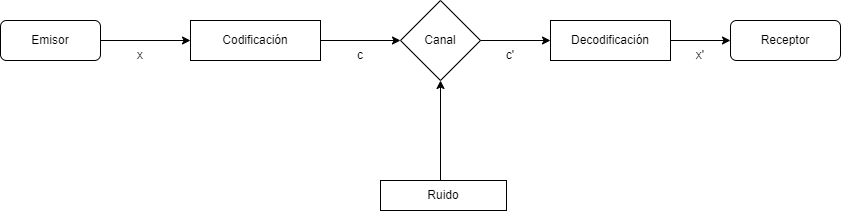
\includegraphics[scale=0.5]{img/canal_comunicacion.png}
	\caption{Canal de Comunicación, \cite{Podesta_2006}.}
     \label{fig:uno}
\end{figure}


La Teoría de Códigos Autocorrectores se ocupa del segundo y cuarto pasos del esquema anterior, es decir, de la codificación y decodificación de mensajes, junto con el problema de
detectar y corregir errores. A veces no es posible pedir retransmisión de mensajes y es por eso que los códigos autocorrectores son tan útiles y necesarios. \cite{Podesta_2006}


%\spacedlowsmallcaps{Estado del arte}



\spacedlowsmallcaps{Descripción y Estructura del proyecto}

Realizaremos una descripción del proyecto realizado a través de las diferentes partes que podemos distinguir en esta memoria:

El primer capítulo sirve como introducción a las herramientas y conceptos que van a ser utilizados frecuentemente a lo largo del resto de capítulos. Se recoge la teoría que será necesaria para el desarrollo del proyecto.

A continuación se presentan y explican los códigos lineales y cíclicos junto a sus propiedades. Analizamos las características necesarias y más relevantes para realizar una buena detección y correción de errores como es encontrar una cota para la distancia mínima de un código. Así, describiremos una familia de códigos cíclicos que tienen una cota muy conocida que es la cota BCH. Además, se realiza la decodificación de este tipo de códigos.

En el tercer capítulo se presenta el anillo de los polinomios torcidos con coeficientes en un cuerpo, cuya diferencia con el anillo de los polinomios usuales radica en el uso de un automorfismo del cuerpo que transforma la multiplicación y ya no es conmutativa. Por tanto, se observan diferencias tanto en la factorización de polinomios como en la evaluación de éstos. Se realiza un estudio de todas estas propiedades.

Durante el cuarto capítulo, utilizaremos la teoría vista en las anteriores secciones y la aplicaremos para conseguir un nuevo tipo de códigos que son los códigos torcidos. Se verá paso a paso la construcción de estos con ejemplos representativos. Además también definiremos la familia de los códigos Reed-Solomon torcidos y su ligera diferencia en construcción con los demás códigos torcidos. Finalmente, se estudia un algoritmo de decodificación para estos códigos y como se pueden corregir errores cometidos en el envío de mensajes.

Para terminar, en el último capítulo, se discutirán aspectos del trabajo, así como los objetivos alcanzados y mejoras a la memoria con el fin de seguir investigando en este campo. 




\spacedlowsmallcaps{Objetivos del trabajo}

En esta sección, se recogen los objetivos que se pretenden realizar en este trabajo.

\begin{itemize}
    \item Estudiar la teoría básica de códigos lineales y cíclicos.
    \item Estudiar el anillo de los polinomios torcidos.
    \item Estudiar los códigos Reed-Solomon torcidos.
    \item Estudiar el Algoritmo de Sugiyama y su implementación para códigos Reed-Solomon torcidos.    
\end{itemize}


% Capítulo donde expongo conceptos de cuerpos finitos, incluyendo
% definiciones como ideal, polinomio irreducible, polinomio mínimo...

\chapter{Preliminares}

En el desarrollo de este capítulo se explicarán conceptos que nos resultarán útiles durante los demás capítulos. Se ha tomado como referencia \cite{Huffman_Pless_2010}.


\section{Cuerpos finitos}

\begin{definition}

Un \textit{cuerpo} es un conjunto $\mathbb{F}$ con dos operaciones: la suma, +, y el producto, $\cdot$ que satisface las siguientes propiedades.
\begin{enumerate}
	\item Conmutatividad: $a+b = b+a$ y $a \cdot b = b \cdot a$ para $a,b \in \mathbb{F}$.
	\item Existencia de elemento neutro: existen $0,1 \in \mathbb{F}$ tal que  $a+0 = a$ y $a \cdot 1 = a$ para todo $a \in \mathbb{F} $.
	\item Existencia de elemento inverso: existe $a^{-1}$ tal que $a \cdot a^{-1} = 1$ para todo $a \neq 0 \in \mathbb{F}$ y existe $-a$ tal que $a + (-a) = 0$ para todo $a \in \mathbb{F}$.
    \item Asociatividad: $(a+b)+c = a+(b+c)$ y $(a \cdot b) \cdot c = a \cdot (b \cdot c)$ para todo $a,b,c \in \mathbb{F}$.
    \item Distributividad: $a \cdot (b+c) = (a \cdot b) + (a \cdot c)$ para todo $a,b,c \in \mathbb{F}$.
\end{enumerate}
\end{definition}

\begin{definition}
Diremos que un cuerpo $\mathbb{F}$ es \textbf{finito} si $\mathbb{F}$ tiene un número finito de elementos y llamaremos \textbf{orden} de $\mathbb{F}$ al número de elementos. En general, denotaremos un cuerpo con $q$ elementos como $\mathbb{F}_q$
\end{definition}

Si $p$ es primo, los enteros módulos $p$ forman un cuerpo, al que denotaremos $\mathbb{F}_p$. Estos son los ejemplos más sencillos de cuerpos finitos.


La finitud de $\mathbb{F}_q$ implica que existe un entero positivo $p$ tal que $1+1+\cdots + 1$ (p $1$s) es $0$. Este entero $p$ es primo y lo denominaremos la \textit{característica} de $\mathbb{F}_q$. Si $a$ es un entero positivo, denotamos la suma de $1$s en el cuerpo como $a$. Además, si queremos escribir la suma de $\alpha$ $a$ veces en el cuerpo, escribiremos $a\alpha$ o $a \cdot \alpha$, por tanto, vemos que $p\alpha = 0 \thinspace \forall \alpha \in \mathbb{F}_q$. El conjunto de $p$ elementos distintos $\{ 0,1,2,\cdots , (p-1) \}$ de $\mathbb{F}_q$ es isomorfo al cuerpo $\mathbb{F}_p$ de los enteros módulo $p$. Como un cuerpo isomorfo a $\mathbb{F}_p$ está contenido en $\mathbb{F}_q$ , diremos que $\mathbb{F}_p$ es un subcuerpo de $\mathbb{F}_q$. A este subcuerpo $\mathbb{F}_p$ lo llamaremos \textit{subcuerpo primo} de $\mathbb{F}_q$. El cuerpo $\mathbb{F}_q$ es además un espacio de dimensión finita sobre $\mathbb{F}_p$, digamos de dimensión $m$. Por lo tanto, $q = p^m$ ya que es el número de vectores en el espacio vectorial de dimensión $m$ sobre $\mathbb{F}_p$.

Resumimos ahora en un teorema los resultados que acabamos de ver.

\begin{theorem}
Sea $\mathbb{F}_q$ un cuerpo finito con q elementos. Entonces :
\begin{enumerate}
	\item $q = p^m$ para algún primo p.
	\item $\mathbb{F}_q$ contiene al subcuerpo $\mathbb{F}_p$.
	\item $\mathbb{F}_q$ es un espacio vectorial sobre $\mathbb{F}_p$ de dimensión m.
	\item $p\alpha = 0 \thinspace \forall \alpha \in \mathbb{F}_q$.
	\item $\mathbb{F}_q$ es único salvo isomorfismo.
\end{enumerate}
\end{theorem}

\subsection{Polinomios y el Algoritmo de Euclides}

El conjunto de los polinomios en $x$ con coeficientes en $\mathbb{F}_q$ lo denotaremos como $\mathbb{F}_q[x]$. Este conjunto forma un anillo conmutativo unitario bajo la suma y multiplicación de polinomios. Un anillo conmutativo unitario satisface los mismos axiomas que un cuerpo excepto que los elementos no nulos no es necesario que tengan inversos multiplicativos. De hecho, $\mathbb{F}_q[x]$ es un dominio de integridad, es decir, no tiene divisores de cero ya que es un anillo conmutativo unitario tal que el producto de dos elementos no nulos en el anillo es también no nulo. El anillo $\mathbb{F}_q[x]$ es importante tanto para la construcción de cuerpos finitos como para la construcción de códigos.

Denotaremos a los polinomios en $\mathbb{F}_q[x]$ como $f(x) = \sum_{i=0}^n a_ix^i$, donde $a_i$ son coeficientes del término $a_ix^i$ de grado $i$. El \textit{grado de un polinomio} es el grado más alto de cualquier término con coeficiente no nulo, lo denotaremos como $deg(f(x))$. El coeficiente del término con mayor grado se le conoce como \textit{coeficiente líder}. Diremos que un polinomio es \textit{mónico} si su coeficiente líder es $1$.


Sea $f(x)$ y $g(x)$ polinomios en $\mathbb{F}_q[x]$. Decimos que \textit{f(x) divide a g(x)}, denotado por $f(x) \mid g(x)$, si existe un polinomio $h(x) \in \mathbb{F}_q[x]$ tal que $g(x) = f(x)h(x)$. Al polinomio $f(x)$ se le dice factor o divisor de $g(x)$. El \textit{máximo común divisor} de $f(x)$ y $g(x)$, siendo al menos uno de ellos no nulo, es el polinomio mónico de $\mathbb{F}_q[x]$ con coeficiente más alto que divide tanto a $f(x)$ como a $g(x)$. El máximo común divisor es único y lo denotaremos como $mcd(f(x),g(x))$. Si el $mcd(f(x),g(x)) = 1$, entonces diremos que $f(x)$ y $g(x)$ son primos relativos.

Como con los enteros, también podemos dividir polinomios y obtener un cociente y un resto.

\begin{theorem}[\textbf{Algoritmo de la División}]
Sea $f(x)$ y $g(x)$ polinomios en $\mathbb{F}_q[x]$ con $g(x)$ no nulo.
\begin{enumerate}
	\item Existen dos polinomios únicos $h(x),r(x) \in \mathbb{F}_q[x]$ tales que $f(x) = g(x)h(x) + r(x)$ donde $deg(r(x)) < deg(g(x))$ o $r(x) = 0$.
	\item Si $f(x) = g(x)h(x) + r(x)$ entonces $mcd(f(x),g(x)) = mcd(g(x),r(x))$.
\end{enumerate}
\end{theorem}

Si usamos el Algoritmo de la División recursivamente, podemos encontrar el mcd de dos polinomios cualesquiera, a este método se le conoce como el Algoritmo de Euclides.

\begin{theorem}[\textbf{Algoritmo de Euclides}]
Sea $f(x)$ y $g(x)$ polinomios en $\mathbb{F}_q[x]$ con $g(x)$ no nulo.
\begin{enumerate}
	\item Repetimos la siguiente secuencia hasta que $r_n(x) = 0$ para algún n:
	
	$f(x) = g(x)h_1(x) + r_1(x)$ donde $deg(r_1(x)) < deg(g(x))$
	
	$g(x) = r_1(x)h_2(x) + r_2(x)$ donde $deg(r_2(x)) < deg(r_1(x))$
	
	$r_1(x) = r_2(x)h_3(x) + r_3(x)$ donde $deg(r_3(x)) < deg(r_2(x))$
	
	\[ \vdots \]
	
	$r_{n-3}(x) = r_{n-2}(x)h_{n-1}(x) + r_{n-1}(x)$ donde $deg(r_{n-1}(x)) < deg(r_{n-2}(x))$
	
	$r_{n-2}(x) = r_{n-1}(x)h_{n}(x) + r_{n}(x)$ donde $deg(r_{n}(x)) = 0$
	
	donde el $mcd(f(x),g(x)) = cr_{n-1}(x)$, donde $c \in \mathbb{F}_q$ es escogido tal que $cr_{n-1}(x)$ sea mónico.
	\item Existen polinomios $a(x),b(x) \in \mathbb{F}_q[x]$ tales que 
	
	$a(x)f(x) + b(x)g(x) = mcd(f(x),g(x))$.
		
\end{enumerate}
\end{theorem}

\begin{exampleth}
Vamos a calcular el $mcd(x^8+x^6+x^5+x^3+x^2+1,x^4+x^3+1)$ en el anillo $\mathbb{F}_2[x]$ usando el Algoritmo de Euclides. La parte 1) del algoritmo produce lo siguiente:

	$x^8+x^6+x^5+x^3+x^2+1 = (x^4+x^3+1)(x^4+x^3+x) + (x^2+x+1)$
	
	$x^4+x^3+1 = (x^2+x+1)(x^2+1) + x $
	
	$x^2+x+1 = x(x+1) + 1$
	
	$x = 1x + 0$
	
Por tanto, $ 1 = mcd(x,1) = mcd(x^2+x+1,x) = mcd(x^4+x^3+1,x^2+x+1) = mcd(x^8+x^6+x^5+x^3+x^2+1,x^4+x^3+1)$. Ahora encontramos $a(x),b(x)$ tales que $a(x)(x^8+x^6+x^5+x^3+x^2+1) + b(x)(x^4+x^3+1) = 1$ haciendo a la inversa los pasos anteriores. Luego, tenemos que :

$ (x^2+x+1) - x(x+1) = 1$

Ahora, despejamos $x$ de la segunda ecuación y lo sustituimos en la tercera lo que quedaría de la siguiente forma,

$ (x^2+x+1) - [(x^4+x^3+1) - (x^2+x+1)(x^2+1)](x+1) = 1$

$(x^2+x+1)(x^3+x^2+x) + (x^4+x^3+1)(x+1) = 1$

Despejamos $(x^2+x+1)$ de la primera ecuación y lo sustituimos en lo que hemos obtenido en el paso anterior, quedando de la siguiente forma,

$[(x^8+x^6+x^5+x^3+x^2+1) - (x^4+x^3+1)(x^4+x^3+x)](x^3+x^2+x) + (x^4+x^3+1)(x+1) = 1 $

$(x^3+x^2+x)(x^8+x^6+x^5+x^3+x^2+1) + (x^7+x^3+x^2)(x^4+x^3+1) = 1$

Por tanto, tenemos que $a(x) = (x^3+x^2+x)$ y $b(x) = (x^7+x^3+x^2)$.
\end{exampleth}

\subsection{Elementos primitivos}

Queremos encontrar una forma sencilla de poder sumar y multiplicar los elementos de un cuerpo $\mathbb{F}_q$. Vimos que $\mathbb{F}_q$ es un espacio vectorial sobre $\mathbb{F}_p$ de dimensión m, luego una forma sencilla de sumar es escribir los elementos como m-tuplas de $\mathbb{F}_p$, sin embargo, la multiplicación no es tan sencilla. Por ello, presentamos el siguiente teorema en donde escribiremos los elementos de otra forma que nos facilite la multiplicación.

\begin{theorem}
\label{th:elementos_primitivos}
Se verifica lo siguiente:
\begin{enumerate}
	\item El grupo $\mathbb{F}_q^*$ es cíclico de orden $q-1$ bajo la multiplicación en $\mathbb{F}_q$.
	\item Si $\gamma$ es un generador de ese grupo cíclico, entonces
	\[  \mathbb{F}_q = \{ 0, 1 = \gamma^0, \gamma, \gamma^2 , \cdots, \gamma^{q-2} \}\]
	
	donde $\gamma^i = 1$ si y solo si $(q-1) \mid i $.
\end{enumerate}
\end{theorem}

\begin{proof}
Por el Teorema Fundamental de Grupos Abelianos Finitos, sabemos que $\mathbb{F}_q^*$ es producto directo de grupos cíclicos de orden $m_1,m_2, \cdots , m_a$, donde $m_i \mid m_{i+1}$ para $1 \leq i < a$ y $m_1m_2 \cdot \cdot \cdot m_a = q-1$. En particular, $\alpha^{m_a} = 1 \thinspace \thinspace \forall \alpha \in \mathbb{F}_q^*$. Luego, el polinomio $x^{m_a} - 1$ tiene al menos $q-1$ raíces, lo cual no es posible a menos que $a = 1$ y $m_a = q-1$. Por tanto, $\mathbb{F}_q^*$ es cíclico, dando lugar a 1).  2) se obtiene como propiedades de los grupos cíclicos.
\end{proof}
 
\begin{definition}
Llamaremos \textbf{elemento primitivo} de $\mathbb{F}_q$ a cada generador $\gamma$ de $\mathbb{F}_q^*$
\end{definition}

Cuando los elementos no nulos de un cuerpo finito son expresados como potencias de $\gamma$, la multiplicación en el cuerpo se puede realizar fácilmente de la siguiente manera, $\gamma^i\gamma^j = \gamma^{i+j} = \gamma^s$, donde $0 \leq s \leq q-2$ y $i+j \equiv s \thinspace ( mod \thinspace q-1)$.



Sea $\gamma$ un elemento primitivo de $\mathbb{F}_q$, entonces $\gamma^{q-1} = 1$ por definición. Por tanto, $(\gamma^s)^{q-1} = 1$ para $0 \leq s \leq q-2$, mostrando que los elementos de $\mathbb{F}_q^*$ son raíces de $x^{q-1}-1 \in \mathbb{F}_q[x]$ y por tanto, de $x^q-x$. Como $0$ es una raíz de $x^q-x$, los elementos de $\mathbb{F}_q$ son precisamente las raíces de $x^q-x$.

\begin{theorem}
\label{th:elementos_cuerpo}
Los elementos de $\mathbb{F}_q$ son precisamente las raíces de $x^q-x$.
\end{theorem}


Para analizar la estructura de un cuerpo, será útil saber el número de elementos primitivos que hay en $\mathbb{F}_q$ y como encontrarlos todos conociendo uno de ellos. Ya que $\mathbb{F}_q^*$ es cíclico, vamos a recordar algunos hechos de los grupos cíclicos finitos.

En cualquier grupo cíclico finito $\mathcal{G}$ de orden n con generador g,  los generadores de $\mathcal{G}$ son precisamente los elementos $g^i$ donde $mcd(i,n) = 1$. Sea $\phi(n)$ el número de enteros i con $ 1 \leq i \leq n$ tal que $mcd(i,n) = 1$. A $\phi$ se le conoce como \textbf{función $\phi$ de Euler} o \textbf{función totiente de Euler}. Así que, $\phi(n)$ generadores de $\mathcal{G}$. El orden de un elemento   $\alpha \in \mathcal{G}$  es el entero positivo más pequeño tal que $\alpha^i = 1$. Un elemento de $\mathcal{G}$ tiene orden $d$ si y solo si $d \mid n$. Además $g^i$ tiene orden $d = n/mcd(i,n)$ y hay tantos $\phi(d)$ elementos de orden $d$. Cuando hablamos de elementos de un cuerpo $\alpha \in \mathbb{F}_q^*$, el orden de $\alpha$ es su orden en el grupo multiplicativo $\mathbb{F}_q^*$. En particular, los elementos primitivos de $\mathbb{F}_q$ son aquellos con orden $q-1$.


\begin{theorem}
Sea $\gamma$ un elemento primitivo de $\mathbb{F}_q$.
\begin{enumerate}
	\item Hay $\phi(q-1)$ elementos primitivos en $\mathbb{F}_q$, esos son los elementos $\gamma^i$ donde $mcd(i,q-1)=1$.
	\item Para cualquier d donde $d \mid (q-1)$, hay $\phi(d)$ elementos en $\mathbb{F}_q$ de orden d y esos son los elementos $\gamma^{(q-1)i/d}$ donde $mcd(i,q) = 1$.
\end{enumerate}
\end{theorem}

\begin{definition}
Un elemento $\tau \in \mathbb{F}_q$ es una \textbf{raíz n-ésima de la unidad} si $\tau^n = 1$ y es una \textbf{raíz n-ésima primitiva de la unidad} si además $\tau^s \neq 1$ para $ 0 < s < n$.
\end{definition}

\subsection{Construcción de cuerpos finitos}

Un polinomio no contante $f(x) \in \mathbb{F}_q[x]$ es irreducible sobre $\mathbb{F}_q$ si no factoriza en un producto de dos polinomios no constantes en $\mathbb{F}_q[x]$ de menor grado. Los polinomios irreducibles en $\mathbb{F}_q[x]$ toman el rol de los números primos en el anillo de los enteros. Por ejemplo, cada entero mayor que $1$ se puede descomponer de forma única en producto de primos positivos. Un resultado similar ocurre en $\mathbb{F}_q[x]$, por lo que tenemos un \textbf{dominio de factorización única}.


\begin{theorem}
\label{th:factorizar_f}
Sea $f(x) \in \mathbb{F}_q[x] $ un polinomio no constante. Entonces, 
\[
f(x) = p_1(x)^{a_1}p_2(x)^{a_2}\cdot \cdot \cdot p_k(x)^{a_k} ,
\]
donde cada $p_i(x)$ es irreducible, los $p_i(x)$s son únicos salvo multiplicación escalar y los $a_i$s son únicos.
\end{theorem}

Además de ser un dominio de factorización única, es un dominio de ideales principales. Un \textbf{ideal} $\mathcal{I}$ en un anillo conmutativo $\mathcal{R}$ es un subconjunto no vacío del anillo el cual es cerrado para la suma, y para el producto por elementos de $\mathcal{I}$ por un elemento de $\mathcal{R}$ siempre se queda en $\mathcal{I}$. El ideal $\mathcal{I}$ es \textbf{principal} si hay un $ a \in \mathcal{R}$ tal que $\mathcal{I} = \{ ra \mid \thinspace r \in \mathcal{R} \}$. Un dominio de ideales principales es un dominio de integridad en donde cada ideal es principal.

 Para construir un cuerpo con característica $p$, empezamos con un polinomio $f(x) \in \mathbb{F}_p[x]$ que sea irreducible en $\mathbb{F}_p$. Supongamos que $f(x)$ es de grado $m$. Usando el Algoritmo de Euclides podemos probar que el anillo cociente $ \mathbb{F}_p[x]/(f(x))$ es un cuerpo y por tanto, $\mathbb{F}_q$ es un cuerpo finito con $q = p^m$ elementos. 
 
 Cada elemento del anillo cociente es una clase de equivalencia $g(x)+f(x)$, donde $g(x)$ está determinado por un grado a lo sumo $m-1$. Podemos comprimir la notación escribiendo las clases como un vector en $\mathbb{F}_p^m$ con la siguiente correspondencia : 
 \[
 g_{m-1}x^{m-1} + g_{m-2}x^{m-2} + \cdots + g_1x + g_0 + (f(x)) \Leftrightarrow g_{m-1}g_{m-2}\cdots g_1g_0 
 \]
 
Con esta notación podemos sumar usando la operación de adición ordinario de los vectores.

Para multiplicar $g_1 + (f(x)) \cdot g_2 + (f(x))$, primero usamos el Algoritmo de la División, obteniendo $g_1(x)g_2(x) = f(x)h(x)+r(x)$ con $deg(r(x)) \leq m-1$ o $r(x) = 0$. Entonces $(g_1 + (f(x)))(g_2 + (f(x))) = r(x) + (f(x))$. La notación es un poco engorrosa así que la vamos a simplificar reemplazando $x$ por $\alpha$ tal que $f(\alpha) = 0$. Así tenemos la correspondencia anterior de la siguiente manera :

\[
g_{m-1}g_{m-2}\cdots g_1g_0  \Leftrightarrow g_{m-1}\alpha^{m-1} + g_{m-2}\alpha^{m-2} + \cdots + g_1\alpha + g_0 
 \]

Así que para multiplicar en $\mathbb{F}_q$, simplemente multiplicamos polinomios en $\alpha$ de manera ordinaria y usamos que $f(\alpha) = 0$ para reducir las potencias de $\alpha$ mayores que $m-1$ a polinomios en $\alpha$ con menor grado que $m$.

\begin{exampleth}
El polinomio $f(x) = x^3+x^2+1$ es irreducible en $\mathbb{F}_2$, si fuese reducible habría un factor de grado 1 que además sería raíz en $\mathbb{F}_2$ y no lo hay. Así que $\mathbb{F}_8 = \mathbb{F}_2/(f(x))$ y usando ambas correspondencias obtenemos que los elementos de $\mathbb{F}_8$ son los que se encuentran en la Tabla \ref{ta:uno}.

\begin{table}
\begin{tabular}{ c | c | c | c}
	Clases & Vectores & Polinomios en $\alpha$ & Potencias de $\alpha$ \\ \hline
	$0+(f(x))$ & 000 & 0 & 0 \\
	$1+(f(x))$ & 001 & 1 & $1=\alpha^0$ \\ 
	$x+(f(x))$ & 010 & $\alpha$ & $\alpha$ \\
	$x+1 +(f(x))$ & 011 & $\alpha +1$ & $\alpha^5$ \\
	$x^2+(f(x))$ & 100 & $\alpha^2$ & $\alpha^2$ \\
	$x^2+1 +(f(x))$ & 101 & $\alpha^2+1$ & $\alpha^3$ \\
	$x^2+x +(f(x))$ & 110 & $\alpha^2+\alpha$ & $\alpha^6$ \\ 
	$x^2+x+1 +(f(x))$ & 111 & $\alpha^2+\alpha+1$ & $\alpha^4$

\end{tabular}
\caption{\label{ta:uno} Elementos de $\mathbb{F}_8$}
\end{table}
	
	Las potencias de $\alpha$ las hemos obtenido de $f(\alpha) = \alpha^3+\alpha^2+1 = 0$ lo que implica que $\alpha^3 = \alpha^2 + 1$, así $\alpha^4 = \alpha\alpha^3 = \alpha(\alpha^2 +1) = \alpha^3+\alpha = \alpha^2 +\alpha + 1$, $\alpha^5 = \alpha\alpha^4 = \alpha(\alpha^2 +\alpha + 1) = \alpha^3+\alpha^2 + \alpha = \alpha^2 + 1 + \alpha^2 +\alpha = \alpha + 1$ y $\alpha^6 = \alpha \alpha^5 = \alpha(\alpha + 1) = \alpha^2 + \alpha$.

Luego, si queremos sumar $x^2+(f(x))$ y $x^2+1+(f(x))$ eso nos da $1+(f(x))$ que corresponde a sumar $100$ y $101$ que da $001$ en $\mathbb{F}_2^3$.

Si ahora queremos multiplicar $x^2+x +(f(x))$ y $x^2+x+1+(f(x))$, multiplicamos $\alpha^6 \cdot \alpha^4  = \alpha^3 = \alpha^2 + 1$ lo que nos da $x^2+1 + (f(x))$.

\end{exampleth}

Describimos la construcción diciendo que $\mathbb{F}_q$ se obtiene a partir de $\mathbb{F}_p$ ``adjuntando'' una raíz $\alpha$ de $f(x)$ a $\mathbb{F}_p$. Esta raíz $\alpha$ normalmente viene dada por $\alpha = x + (f(x))$ en el anillo cociente $\mathbb{F}_p[x]/(f(x))$ y por tanto, $g(x) + (f(x)) = g(\alpha)$ y $f(\alpha) = f(x + (f(x))) = f(x) + (f(x)) = 0 + (f(x))$. 

En general, $\alpha$ no tiene que ser un elemento primitivo. Decimos que un polinomio irreducible en $\mathbb{F}_p$ con grado $m$ es primitivo, si tiene una raíz que es un elemento primitivo de $\mathbb{F}_q = \mathbb{F}_{p^m}$. Idealmente, queremos empezar con un polinomio primitivo para construir nuestro cuerpo, pero no es un requisito. Además, el polinomio con el que empezamos si lo multiplicamos por una constante para hacerlo mónico, no influye en el ideal generado por el polinomio o el anillo cociente. Tenemos el siguiente resultado:

\begin{theorem}
Para cualquier primo p y cualquier entero positivo m, existe un cuerpo finito, único salvo isomorfismos, tal que tiene $q = p^m$ elementos. 
\end{theorem}

\subsection{Automorfismos}


Los automorfismos de $\mathbb{F}_q$ forma un grupo con la composición.

\begin{definition}
Un \textbf{automorfismo} $\sigma$ de $\mathbb{F}_q$ es una aplicación biyectiva $\sigma : \mathbb{F}_q \rightarrow \mathbb{F}_q$ tal que $\sigma(\alpha+\beta) = \sigma(\alpha) + \sigma( \beta)$ y $\sigma(\alpha \beta) =\sigma(\alpha)\sigma(\beta) \thinspace \forall \alpha , \beta \in \mathbb{F}_q$. 

\end{definition}


Definimos $\sigma_p : \mathbb{F}_q \rightarrow \mathbb{F}_q$ como 
\[ 
\sigma_p (\alpha) = \alpha^p \thinspace \forall \alpha \in \mathbb{F}_q
\]

Obviamente, $\sigma_p(\alpha \beta) =\sigma_p(\alpha)\sigma_p(\beta)$ y $\sigma_p(\alpha+\beta) = \sigma_p(\alpha) + \sigma_p( \beta)$. Como $\sigma_p$ tiene núcleo $\{ 0 \}$, $\sigma_p$ es un automorfismo de $\mathbb{F}_q$, al que llamaremos \textbf{automorfismo de Frobenius}. Análogamente, definimos $\sigma_{p^r} (\alpha) = \alpha^{p^r}$.

El grupo de los automorfimos de $\mathbb{F}_q$, denotado por $Gal(\mathbb{F}_q)$, se le llama grupo de Galois de $\mathbb{F}_q$. Con el siguiente teorema vamos a caracterizar ese grupo.

\begin{theorem}
\begin{enumerate}
	\item $Gal(\mathbb{F}_q)$ es cíclico de orden $m$ y está generado por el automorfismo de Frobenius $\sigma_p$.
	\item El subcuerpo primo de $\mathbb{F}_q$ es precisamente el conjunto de elementos de $\mathbb{F}_q$ tal que $\sigma_p(\alpha) = \alpha$.
	\item El subcuerpo $\mathbb{F}_q$ de $\mathbb{F}_{q^t}$ es precisamente el conjunto de elementos de $\mathbb{F}_{q^t}$ tal que $\sigma_p(\alpha) = \alpha$.
\end{enumerate}
\end{theorem}

Usamos $\sigma_p$ para denotar al automorfismo de Frobenius de cualquier cuerpo con característica $p$. Si $\mathbb{E}$ y $\mathbb{F}$ son cuerpos de característica $p$ con $\mathbb{E}$ siendo un cuerpo de extensión de $\mathbb{F}$, entonces el automorfismo de Frobenius de $\mathbb{E}$ restringido a $\mathbb{F}$ es el automorfismo de Frobenius de $\mathbb{F}$ 


\begin{definition}
Un elemento $\alpha \in \mathbb{F}$ es \textbf{fijo} si $\sigma(\alpha) = \alpha$ por el automorfismo $\sigma$ de $\mathbb{F}$.
\end{definition}

Sea $ r \mid m$. Entonces $\sigma_{p^r}$ genera un subgrupo cíclico de $Gal(\mathbb{F}_q)$ de orden $m/r$


\subsection{Polinomios mínimos}

Sea $\mathbb{E}$ un cuerpo de extensión finito de $\mathbb{F}_q$, entonces $\mathbb{E}$ es un espacio vectorial sobre $\mathbb{F}_q$ y por tanto, $\mathbb{E} = \mathbb{F}_{q^t}$ para algún entero positivo $t$. Cada elemento $\alpha$ de $\mathbb{E}$ es una raíz del polinomio $x^{q^t}-x$ como dijimos anteriormente. Por consiguiente, hay un polinomio mónico $\mathcal{M}_\alpha(x)$ en $\mathbb{F}_q[x]$ de menor grado el cual tiene a $\alpha$ como raíz. A este polinomio lo llamaremos \textbf{polinomio mínimo} de $\alpha$ sobre $\mathbb{F}_q$. Veamos unas cuantas propiedades sobre los polinomios mínimos. 

\begin{theorem}
\label{th:prop_pol}
Sea $\mathbb{F}_{q^t}$ un cuerpo de extensión de $\mathbb{F}_q$ y sea $\alpha$ un elemento de $\mathbb{F}_{q^t}$ con polinomio mínimo $\mathcal{M}_\alpha(x)$ en $\mathbb{F}_q[x]$. Tenemos lo siguiente:
\begin{enumerate}
	\item $\mathcal{M}_\alpha(x)$ es irreducible sobre $\mathbb{F}_q$.
	\item Si $g(x)$ es cualquier polinomio en $\mathbb{F}_q[x]$  satisfaciendo que $g(\alpha) = 0$, entonces $\mathcal{M}_\alpha(x) \mid g(x)$.
	\item $\mathcal{M}_\alpha(x)$ es único, es decir, solo hay un polinomio mónico en $\mathbb{F}_q[x]$ de menor grado que tiene a $\alpha$ como raíz.
\end{enumerate}
\end{theorem}

Si empezamos con un polinomio irreducible $f(x)$ en $\mathbb{F}_q$ de grado $r$, podemos adjuntar una raíz de $f(x)$ a $\mathbb{F}_q$ para obtener el cuerpo $\mathbb{F}_{q^r}$, en el cual, todas sus raíces se quedan en $\mathbb{F}_{q^r}$ 

\begin{theorem}
\label{th:raices_minimo}
Sea $f(x)$ un polinomio mónico irreducible en $\mathbb{F}_q$ con grado r. Entonces :
\begin{enumerate}
	\item Todas las raíces de $f(x)$ se encuentran en $\mathbb{F}_{q^r}$ y en cualquier cuerpo que contenga a $\mathbb{F}_q$ junto a una raíz de $f(x)$.
	\item $f(x) = \prod_{i=1}^r (x - \alpha^i)$, donde $\alpha^i \in \mathbb{F}_{q^r}$ para $ 1 \leq i \leq r$.
	\item $f(x) \mid x^{q^r}-x$.
\end{enumerate}
\end{theorem}

\begin{proof}
Sea $\alpha$ una raíz de $f(x)$ que adjuntamos a $\mathbb{F}_q$ para formar el cuerpo $\mathbb{E}_\alpha$ con $q^r$ elementos. Si $\beta$ es una raíz de $f(x)$, que no está en $\mathbb{E}_\alpha$, es raíz de algún factor irreducible en $\mathbb{E}_\alpha$ de $f(x)$. Adjuntando $\beta$ a $\mathbb{E}_\alpha$ formamos un cuerpo de extensión $\mathbb{E}$ de $\mathbb{E}_\alpha$. Sin embargo, dentro de $\mathbb{E}$, hay un subcuerpo $\mathbb{E}_\beta$ obtenido al adjuntar $\beta$ a $\mathbb{F}_q$. $\mathbb{E}_\beta$ debe tener $q^r$ elemenetos ya que $f(x)$ es un irreducible de grado $r$ en $\mathbb{F}_q$
. Como $\mathbb{E}_\alpha$ y $\mathbb{E}_\beta$ son subcuerpos de $\mathbb{E}$ del mismo tamaño, entonces $\mathbb{E}_\alpha = \mathbb{E}_\beta$, probando que todas las raíces de $f(x)$ se encuentran en $\mathbb{F}_{q^r}$. Luego, como cualquier cuerpo que contenga a $\mathbb{F}_q$ y una raíz de $f(x)$ contiene a $\mathbb{F}_{q^r}$, queda demostrado 1). Para 2), como las $\alpha_i$ son las raíces de $f(x)$ es simplemente su descomposición en factores. Para el apartado 3) lo sacamos a partir del 2) ya que $x^{q^r}-x = \prod_{\alpha \in \mathbb{F}_{q^r}} (x - \alpha)$ por el Teorema \ref{th:elementos_cuerpo}
\end{proof}
 

En particular, este teorema se puede aplicar a polinomios mínimos ya que estos polinomios son mónicos irreducibles.

\begin{lemma}
\label{le:divisible}
Sea $s = p^r$ y $q = p^m$, entonces $(x^s-x) \mid (x^q-x)$ si y solo si $r \mid m $.
\end{lemma}

\begin{theorem}
Sea $\mathbb{F}_{q^t}$ una extensión de $\mathbb{F}_{q}$ y sea $\alpha$ un elemento de $\mathbb{F}_{q^t}$ con polinomio mínimo $\mathcal{M}_\alpha(x)$ en $\mathbb{F}_q[x]$. Tenemos lo siguiente:
\begin{enumerate}
	\item $\mathcal{M}_\alpha(x) \mid (x^q-x)$.
	\item $\mathcal{M}_\alpha(x)$ tiene raíces distintas todas en $\mathbb{F}_{q^t}$.
	\item El grado de $\mathcal{M}_\alpha(x)$ divide a t.
	\item  $x^{q^t} - x = \prod_\alpha \mathcal{M}_\alpha(x)$, donde $\alpha$ recorre un subconjunto de $\mathbb{F}_{q^t}$ que enumera los polinomios mínimos de todos los elementos de $\mathbb{F}_{q^t}$ exactamente una vez.
	\item $x^{q^t}-x = \prod_f f(x)$, donde f recorre todos los polinomios mónicos irreducibles de $\mathbb{F}_q$ cuyos grados dividen a t.
\end{enumerate}
\end{theorem}

\begin{proof}
El apartado 1) sale del Teorema \ref{th:prop_pol}, ya que $\alpha^{q^t}-\alpha = 0$ por el Teorema \ref{th:elementos_cuerpo}. Como las raíces de $x^{q^t}-x$ son los $q^t$ elementos de $\mathbb{F}_{q^t}$, $x^{q^t}-x$ tiene raíces distintas, luego 1) y por el Teorema \ref{th:raices_minimo} se tiene 2). Por el Teorema \ref{th:factorizar_f}, $x^{q^t}-x = \prod_{i=1}^n p_i(x)$ , donde $p_i(x)$ es irreducible en $\mathbb{F}_{q}$.Como $x^{q^t}-x$ tiene raíces distintas, los factores $p_i(x)$ son distintos. Si los escalamos, podemos asumir que cada uno es mónico ya que $x^{q^t}-x$ es mónico. Así que $p_i(x) = \mathcal{M}_\alpha(x)$ para cualquier $\alpha \in \mathbb{F}_{q^t}$ con $p_i(\alpha) = 0$. Por tanto, tenemos 4). Pero si $\mathcal{M}_\alpha(x)$ tiene grado $r$, adjuntando $\alpha$ a $\mathbb{F}_{q}$ obtenemos el subcuerpo $\mathbb{F}_{q^r} = \mathbb{F}_{p^{mr} }$ o $\mathbb{F}_{q^t} = \mathbb{F}_{p^{mt}}$ lo que implica que $ mr \mid mt$ y por tanto 3). El apartado 5) se obtiene del 4) si demostramos que cada polinomio mónico irreducible de $\mathbb{F}_{q}$ de grado $r$ que divide a $t$ es un factor de $x^{q^t}-x$. Pero $f(x) \mid (x^{q^r}-x)$ por el Teorema \ref{th:raices_minimo}. Y como $mr \mid mt$, $(x^{q^r}-x) | (x^{q^t}-x)$ por el Lema \ref{le:divisible}.

\end{proof}

Dos elementos de $\mathbb{F}_{q^t}$ que tienen el mismo polinomio mínimo en $\mathbb{F}_{q}[x]$ se les llama \textbf{conjugados} en $\mathbb{F}_{q}$. Será importante encontrar todos los conjugados de $\alpha \in \mathbb{F}_{q}$, ya que, estos son todas las raíces de $\mathcal{M}_\alpha(x)$. Podemos encontrarlos con el siguiente teorema.

\begin{theorem}
Sea $f(x)$ un polinomio en $\mathbb{F}_{q}[x]$ y sea $\alpha$ una raíz de $f(x)$ en una extensión $\mathbb{F}_{q^t}$. Entonces:
\begin{enumerate}
	\item $f(x^q) = f(x)^q$.
	\item $\alpha^q$ es también una raíz de $f(x)$ en $\mathbb{F}_{q}$.
\end{enumerate}
\end{theorem}

\begin{proof}
Sea $f(x) = \sum_{i=0}^n a_ix^i$. Como $q = p^m$, donde $p$ es la característica de $\mathbb{F}_{q}$, $f(x)^q = \sum_{i=0}^n a_i^qx^{iq}$. Sin embargo, $a_i^q = a_i$, porque $a_i \in \mathbb{F}_{q}$ y los elementos de $\mathbb{F}_{q}$ son raíces de $x^q-x$ por el Teorema \ref{th:elementos_cuerpo}, hemos probado 1). En particular, $f(\alpha^q) = f(\alpha)^q = 0 $ lo que implica 2). 
\end{proof}

Si repetimos este teorema vemos que $\alpha,\alpha^q,\alpha^{q^2},\cdots $ son todas las raíces de $\mathcal{M}_\alpha(x)$. Este proceso termina tras el término $r$ ya que $\alpha^{q^r} = \alpha$.



%CAPITULO 1 NUEVO


%Añado el apartado de códigos lineales entero, sin embargo, como no vamos a usar los códigos duales, nos lo saltamos.

%Sobre el peso y las distancias, lo voy a añadir pero CAMBIAR la notación del peso a w en vez de wt

%Nos metemos ya en códigos cíclicos, mirar la parte de la factorización de x^n-1 de nuevo, pero lo de las clases q-ciclotómicas si lo voy a dejar tal cual.

%El punto de idempotentes me lo salto ya uqe no nos sirve, sobre los multiplicadores ya veré.

%Sobre los ceros, es importante lo del conjunto de definición.

% en Minima distancia de codigos ciclicos omito las otras técnicas de 
% acotación y dejamos solo la cota BCH que es la que nos interesa. Mirar también el ejemplo sobre la cota BCH

%Quitar en principio la nueva definición de los códigos Reed-Solomon en sentido estricto pero preguntarle a Gabriel si la dejo o no.


\chapter{Introducción a los códigos lineales}

Todo el desarrollo de este capítulo está basado en \cite{Huffman_Pless_2010} y \cite{Wassermann_2006} .
\section{Códigos lineales}

Sea $\mathbb{F}_q$ el cuerpo finito de $q$ elementos, denotamos, $\mathbb{F}_q^n$ al espacio vectorial de las n-tuplas sobre el cuerpo finito $\mathbb{F}_q$. A los vectores $(a_1,a_2,\cdots,a_n)$ de $\mathbb{F}_q$ generalmente los escribiremos como $a_1a_2\cdots a_n$.



\begin{definition}
Un $(n,M)$ \emph{código} $\mathcal{C}$ sobre $\mathbb{F}_q$ es un subconjunto de $\mathbb{F}_q^n$ de tamaño $M$. Llamaremos \emph{palabras código} a los elementos de $\mathcal{C}$.
\end{definition}

\begin{exampleth}
\begin{itemize}
	\item En el cuerpo $\mathbb{F}_2$, a los códigos se les conoce como \emph{códigos binarios} y un ejemplo sería $\mathcal{C} = \{00,01,10,11\}$

	\item En el cuerpo $\mathbb{F}_3$, a los códigos se les conoce como \emph{códigos ternarios} y un ejemplo sería $\mathcal{C} = \{01, 12, 02, 10, 20, 21, 22\}$
\end{itemize}
\end{exampleth}

Si $\mathcal{C}$ es un espacio k-dimensional de $\mathbb{F}_q^n$, entonces decimos que $\mathcal{C}$ es un $\left[n,k\right]$ \emph{código lineal} sobre $\mathbb{F}_q$ y tiene $q^k$ palabras código. Las dos formas más comunes de representar un código lineal son con la \emph{matriz generadora} o la \emph{matriz de paridad}.

\begin{definition}

Una \emph{matriz generadora} de un $\left[n,k\right]$ \emph{código lineal} $\mathcal{C}$ es cualquier matriz $k \times n$ cuyas filas forman una base de $\mathcal{C}$.
\end{definition}

Para cada conjunto de $k$ filas independientes de una matriz generadora $G$, se dice que dicho conjunto de coordenadas forman un \emph{conjunto de información} de $\mathcal{C}$. Las $r = n - k$ coordenadas restantes forman el \emph{conjunto de redundancia} y el número $r$ es la \emph{redundancia} de $\mathcal{C}$.

En general no hay una única matriz generadora pero si las primeras $k$ coordenadas forman un conjunto de información, entonces el código tiene una única matriz generado de la forma $\left[I_k | A\right]$, donde $I_k$ es la matriz identidad $k \times k$. Esta matriz se dice que está en \emph{forma estándar}.

Como un código lineal es un subespacio de un espacio vectorial, es el núcleo de alguna transformación lineal.

\begin{definition}
Una \emph{matriz de paridad} $H$ de dimensión $(n-k) \times k$ es una matriz que verifica que %de un $\left[n,k\right]$ \emph{código lineal} $\mathcal{C}$ es una matriz que verifica :
\[
C = \{ x \in  \mathbb{F}_q^n | Hx^T = 0  \}
\]
\end{definition}

Como ocurría con la matriz generadora, la matriz de paridad no es única. Con el siguiente resultado podremos obtener una de ellas cuando $\mathcal{C}$ tiene una matriz generadora en forma estándar.

\begin{theorem}[Matriz de paridad a partir de la generadora]
\label{th:matriz_paridad}

Si $G = \left[I_k | A\right]$ es una matriz generadora del $\left[n,k\right]$ código $\mathcal{C}$ en su forma estándar, entonces $H = \left[-A^T |I_{n-k}\right]$ es la matriz de paridad de $\mathcal{C}$.
\end{theorem}

\begin{proof}
Sabemos que $HG^T = -A^T + A^T = 0$, luego $\mathcal{C}$ está contenido en el núcleo de la transformación lineal $x \mapsto Hx^T$. Como $H$ tiene rango $n-k$, el núcleo de esta transformación es de dimensión $k$ que coincide con la dimensión de $\mathcal{C}$.
\end{proof}

\begin{exampleth}
 \label{ex:matriz_generadora}
Sea la matriz $G = \left[I_4 | A\right]$, donde

\[
G = \left( \begin{array}{cccc|ccc}
	1 & 0 & 0 & 0 & 0 & 1 & 1 \\
	0 & 1 & 0 & 0 & 1 & 0 & 1 \\
	0 & 0 & 1 & 0 & 1 & 1 & 0 \\
	0 & 0 & 0 & 1 & 1 & 1 & 1 
			\end{array} 
	\right)
\]
es la matriz generadora en forma estándar del $\left[7,4\right]$ código binario que denotaremos por $\mathcal{H}_3$.
Por el Teorema \ref{th:matriz_paridad}, la matriz de paridad de $\mathcal{H}_3$ es

\[
H =  \left[A^T | I_3\right] = \left( \begin{array}{cccc|ccc}
	0 & 1 & 1 & 1 & 1 & 0 & 0 \\
	1 & 0 & 1 & 1 & 0 & 1 & 0 \\
	1 & 1 & 0 & 1 & 0 & 0 & 1 

			\end{array} 
	\right)
\]

Este código se le conoce como el $\left[7,4\right]$ \emph{código de Hamming}.
\end{exampleth}

\section{Pesos y distancias}
\begin{definition}
La \textit{distancia de Hamming} $d(x,y)$ entre dos vectores $x,y \in \mathbb{F}_q^n$ es el número de coordenadas en las que x e y difieren. 
\end{definition}

\begin{exampleth}
	Sea $\mathbf{x}=20110$ y $\mathbf{y}=10121$ entonces $d(x,y)=3$.
\end{exampleth}

%TODO cambiar el teorema por La distancia de Hamming es una distancia en \mathbb{F}_q^n
% y ya en la demostración decir que cumple las 4 propiedades.
\begin{theorem}
	La distancia de Hamming $d(x,y)$ satisface las siguientes cuatro propiedades:
	\begin{enumerate}
	\item No negatividad: $d(x,y) \geq 0 \quad \forall x,y \in \mathbb{F}_q^n$.
	\item $d(x,y)=0 \Leftrightarrow x = y$.
	\item Simetría: $d(x,y)=d(y,x) \quad \forall x,y \in \mathbb{F}_q^n$.
	\item Desigualdad triangular: $d(x,z)\leq d(x,y) + d(y,z) \quad \forall x,y,z \in \mathbb{F}_q^n$.
	\end{enumerate}
	
\end{theorem}

\begin{proof}
Las tres primeras propiedades son evidentes por la definición de la distancia, comprobemos la última propiedad.

Distinguimos dos casos, si $ x = z $ tenemos que $d(x,z) = 0$ y por tanto se verifica la desigualdad. Si $x \neq z$ entonces, no puede ocurrir que $x = y = z $, por tanto $d(x,y) \neq 0$ o $d(y,z) \neq 0$ y por la no negatividad se tendría la desigualdad, en el caso de que $ x = y$ o $y = z$ tendríamos la igualdad.
\end{proof}

Llamaremos \textbf{distancia mínima} de un código $\mathcal{C}$ a la menor distancia entre dos palabras del código. Además, esta distancia es un invariante y es importante a la hora de determinar la capacidad de corrección de errores del código $\mathcal{C}$ .

\begin{exampleth}
Sea $\mathcal{C} = \left\{ 201310, 311210, 202210, 312100 \right\} $ un código. Sus distancias son:
\[
d(201310, 311210) = 3 , \quad d(201310,202210) = 2, \quad d(201310,312100) = 5,
\]
\[
 d(311210, 202210) = 3, \quad d(311210,312100) = 3, \quad d(202210,312100) = 4 
\]
Luego, la distancia mínima es $d(\mathcal{C}) = 2$.
\end{exampleth}

\begin{definition}
El \textbf{peso de Hamming}, denotado por $\operatorname{wt}(x)$, de un vector $x \in \mathbb{F}_q^n$ es el número de coordenadas no-nulas en $x$. Llamaremos \textit{peso de $\mathcal{C}$} a 
$\operatorname{wt}(\mathcal{C}) = \min(\operatorname{wt}(x))$ con $x \neq 0 $.
\end{definition}

\begin{exampleth}
	Sea $\mathbf{x} = 202210$ un vector en $\mathbb{F}_3^6$ entonces $\operatorname{wt}(x) = 4$.
\end{exampleth}

\begin{theorem}
Si $x,y \in \mathbb{F}_q^n$, entonces $d(x,y) = \operatorname{wt}(x-y)$. Si $\mathcal{C}$ es un código lineal, la distancia mínima $d$ es igual al peso mínimo de $\mathcal{C}$.
\end{theorem}

\begin{proof}
Como $\mathcal{C}$ es lineal, tenemos que $ 0 \in \mathcal{C}$ y además $\operatorname{wt}(x) = d(x,0) \quad \forall x \in \mathcal{C}$, luego $d(\mathcal{C}) \leq \operatorname{wt}(\mathcal{C})$.

Por otro lado, sea $x,y \in \mathcal{C}$ entonces $x-y \in \mathcal{C} \quad \forall x,y \in \mathcal{C}$ y sabemos que $d(x,y) = \operatorname{wt}(x-y) \geq \operatorname{wt}(\mathcal{C})$ para cualesquiera $x,y \in \mathcal{C}$. Se tiene que $d(\mathcal{C}) \geq \operatorname{wt}(\mathcal{C})$.

Hemos conseguido así la igualdad, $d(\mathcal{C}) = \operatorname{wt}(\mathcal{C})$.
\end{proof}

Como resultado de este teorema, para códigos lineales, la \textbf{ distancia mínima}  también se denomina el \textbf{peso mínimo} de un código. Si se conoce el peso mínimo de un código entonces nos referiremos a él como el $\left[n,k,d\right]$ código.


\section{Códigos cíclicos}

Vamos a estudiar los códigos cíclicos de longitud n, por ello, denotaremos las coordenadas de sus posiciones como $0,\cdots,n-1$ que son los enteros módulo n.

\begin{definition}
 Un código lineal $\mathcal{C}$ de longitud n sobre $\mathbb{F}_q$ es \textit{cíclico} si para cada vector $c = c_0\cdots c_{n-2}c_{n-1}$ en  $\mathcal{C}$, el vector $c_{n-1},c_0,\cdots,c_{n-2}$ obtenido de \textbf{c} por la permutación de las coordenadas $ i \rightarrow i+1 (\thinspace mod \thinspace n)$, está también en $\mathcal{C}$.
 \end{definition}
 
 Así, un código cíclico contiene las n permutaciones cíclicas de cada palabra código. Por tanto, es conveniente pensar que las coordenadas cuando alcanzan $n-1$, vuelven a la coordenada $0$.

Cuando hablemos de códigos cíclicos sobre $\mathbb{F}_q$, normalmente las palabras códigos las representaremos en su forma polinómica, ya que hay un isomorfismo de $\mathbb{F}_q$-espacios vectoriales entre los vectores $c = c_0c_1\cdots c_{n-1}$ en $\mathbb{F}_q^n$ y los polinomios $c(x)=c_0+c_1x+\cdots+c_{n-1}x^{n-1}$ en $\mathbb{F}_q[x]$ con grado como mucho $n-1$. Notemos que si \textbf{c} es el polinomio dado, entonces $xc(x)=c_{n-1}x^{n}+c_0x+c_1x^2+\cdots+c_{n-2}x^{n-1}$ representa una permutación de \textbf{c} si $x^n$ es igual a $1$. Más formalmente, el hecho de que el código cíclico $\mathcal{C}$ sea invariante por permutaciones, implica que, $c(x)$ está en $\mathcal{C}$, entonces $xc(x)$ también lo está. 

Esto sugiere que para un mejor estudio de los códigos cíclicos, desarrollemos el anillo cociente \[ \mathcal{R}_n =\mathbb{F}_q[x] / (x^n-1).\] Bajo la correspondencia vectores-polinomios dada anteriormente, los códigos cíclicos son ideales de $\mathcal{R}_n$ y los ideales de $\mathcal{R}_n$ son códigos cíclicos. Luego, el estudio de códigos cíclicos en $\mathbb{F}_q^n$ es equivalente al estudio de los ideales de $\mathcal{R}_n$. Para este estudio necesitamos factorizar el polinomio $x^n-1$.

\subsection{Factorización de $x^n-1$ }
Queremos encontrar los factores irreducibles de $x^n-1$. Encontramos dos posibilidades: que $x^n-1$ tenga factores irreducibles repetidos o no los tenga. En el caso de los códigos cíclicos, se centra más en el segundo caso ya que en el primero, las capacidades de correción son peores por lo que no es tan interesante, por ello, hacemos la asumpción de que $x^n-1$ no tiene factores repetidos, que es equivalente a que \textit{q} y \textit{n} son primos relativos.

Como ayuda para factorizar $x^n-1$ sobre $\mathbb{F}_q^n$, es útil considerar la extensión $\mathbb{F}_{q^t}^n$ sobre $\mathbb{F}_q^n$ que contiene todas las raíces del polinomio. En otras palabras, $\mathbb{F}_{q^t}^n$ debe contener las raíces primitivas \textit{n-ésimas} de la unidad, que ocurre cuando $ n \mid (q^t-1)$.  Definimos el orden, $ord_n(q)$ de \textit{q} módulo \textit{n}, como el entero positivo más pequeño \textit{a} tal que $q^a \equiv 1 \thinspace ( mod \thinspace n)$. Notemos que si $t = ord_n(q)$, entonces $\mathbb{F}_{q^t}^n$ contiene la raíz primitiva \textit{n-ésima} de la unidad $\alpha$ , pero ninguna extesión del cuerpo $\mathbb{F}_q^n$ contiene esa raíz. Como los $\alpha^i$ son distintos para $0 \leq i < n $ y $(\alpha^i)^n = 1$ , entonces $\mathbb{F}_{q^t}^n$ contiene todas las raíces de $x^n-1$. Consecuentemente, llamaremos a $\mathbb{F}_{q^t}^n$ el \textit{cuerpo de descomposición} de $x^n-1$ sobre $\mathbb{F}_q^n$. Así que los factores irreducibles de $x^n-1$ sobre $\mathbb{F}_q^n$ deben de ser productos de los distintos polinomios mínimos de las raíces \textit{n-ésimas} en $\mathbb{F}_{q^t}^n$.  Supongamos que $\gamma$ es un elemento primitivo, es decir, el elemento generador de $\mathbb{F}_{q^t}^n$, entonces $\alpha = \gamma^d$ es una raíz primitiva \textit{n-ésima} de la unidad en donde $d = (q^t-1)/n$. Las raíces de $\mathcal{M}_{\alpha^s}(x)$ son $\{ \gamma^{ds}, \gamma^{dsq},\gamma^{dsq^2} ,\cdots, \gamma^{dsq^{r-1}} \} = \{ \alpha^s,\alpha^{sq},\alpha^{sq^2},\cdots,\alpha^{sq^{r-1}} \}$ donde \textit{r} es el entero positivo más pequeño que cumple que $dsq^r \equiv ds \thinspace ( mod \thinspace q-1 )$ pero esto se verifica si y solo si $sq^r \equiv s \thinspace ( mod \thinspace n )$


\begin{definition}
Sea $\mathbb{F}_q^n$ un cuerpo finito y $\mathbb{F}_{q^t}^n$ una extensión de $\mathbb{F}_q^n$, llamaremos \textit{clase q-ciclotómica de s módulo n} al conjunto :
\[
	\mathcal{C}_s = \{s,sq,\cdots,sq^{r-1} \} \thinspace (mod \thinspace n)
\]
donde \textit{r} es el menor entero positivo tal que $sq^r \equiv s \thinspace (mod \thinspace n ) $.
\end{definition}

Las distintas clases \textit{q-ciclotómicas} modulo \textit{n} forman una partición del conjunto de los enteros $\{0,1,2,\cdots,n-1\}$.

\begin{exampleth}
\label{ex: clase_mod_quince}
 Vamos a calcular las clases \textit{2-ciclotómicas} para $n=21$ y $q=2$ :

La primera de todas es $\mathcal{C}_0 = \{ 0*2^r \equiv 0 \thinspace (mod \thinspace 21) \} = \{ 0 \} $ y repetimos este proceso. Luego tenemos:

$\mathcal{C}_1 = \{ 1*2^r \equiv 1 \thinspace (mod \thinspace 21) \} = \{ 1, 1*2^1=2, 1*2^2 = 4, 1*2^3 = 8, 1*2^4 = 16,1*2^5 = 11 \} = \{1,2,4,8,11,16\} $
ya que $1*2^6 = 64 \equiv 1 \thinspace (mod \thinspace 21)$ luego $r=6$.

$\mathcal{C}_3 = \{ 3*2^r \equiv 3 \thinspace (mod \thinspace 21) \} = \{ 3,3*2 = 6, 3*2^2 = 12\} = \{3,6,12 \} $ ya que $3*2^3 = 24 \equiv 3 \thinspace (mod \thinspace 21 )$ luego $r=3$.

$\mathcal{C}_5 = \{ 5*2^r \equiv 5 \thinspace (mod \thinspace 21) \} = \{ 5, 5*2=10,5*2^2 = 20, 5*2^3 = 19, 5*2^4 = 17,5*2^5 = 13 \} = \{5,10,13,17,19,20\} $
ya que $5*2^6 = 320 \equiv 5 \thinspace (mod \thinspace 21)$ luego $r=6$.

$\mathcal{C}_7 = \{ 7*2^r \equiv 7 \thinspace (mod \thinspace 21) \} = \{ 7,7*2 = 14 \} = \{ 7,14 \} $ ya que $7*2^2 = 28 \equiv 7 \thinspace (mod \thinspace 21 )$ luego $r=2$.

$\mathcal{C}_9 = \{ 9*2^r \equiv 9 \thinspace (mod \thinspace 21) \} = \{ 9,9*2 = 18,9*2^2 = 15 \} = \{ 9,15,18 \} $ ya que $9*2^3 = 72 \equiv 9 \thinspace (mod \thinspace 21 )$ luego $r=3$.

\end{exampleth}

\begin{exampleth} 
\label{ex:clase_mod_ocho}
Vamos a calcular las clases \textit{3-ciclotómicas} para $n=8$ y $q=3$ que serán las siguientes :

$\mathcal{C}_0 = \{ 0*3^r \equiv 0 \thinspace (mod \thinspace 8) \} = \{ 0 \} $

$\mathcal{C}_1 = \{ 1*3^r \equiv 1 \thinspace (mod \thinspace 8) \} = \{ 1, 1*3^1=3 \} = \{1,3\} $
ya que $1*3^2 = 9 \equiv 1 \thinspace (mod \thinspace 8)$ luego $r=2$.

$\mathcal{C}_2 = \{ 2*3^r \equiv 2 \thinspace (mod \thinspace 8) \} = \{ 2, 2*3^1=6 \} = \{2,6\} $
ya que $2*3^2 = 18 \equiv 2 \thinspace (mod \thinspace 8)$ luego $r=2$.

$\mathcal{C}_4 = \{ 4*3^r \equiv 4 \thinspace (mod \thinspace 8) \} = \{ 4 \} $
ya que $4*3^1 = 12 \equiv 4 \thinspace (mod \thinspace 8)$ luego $r=1$.

$\mathcal{C}_5 = \{ 5*3^r \equiv 5 \thinspace (mod \thinspace 8) \} = \{ 5, 5*3^1=7 \} = \{5,7\} $
ya que $5*3^2 = 45 \equiv 5 \thinspace (mod \thinspace 8)$ luego $r=2$.

Luego, ya tenemos todas las clases \textit{3-ciclotómicas} para $n=8$ y $q=3$.

\end{exampleth}



\begin{theorem}
\label{th:factorizar_xn}
Sea \textit{n} un entero positivo, primo relativo con \textit{q}. Sea $t = ord_n(q)$ y sea $\alpha$ la raíz primitiva \textit{n-ésima} de la unidad en $\mathbb{F}_{q^t}$.
\begin{enumerate}

	\item Por cada entero \textit{s} con $0 \leq s < n$, el polinomio mínimo de $\alpha^s$ sobre  $\mathbb{F}_q$ es
	\[
	\mathcal{M}_{\alpha^s}(x) = \prod_{i \in \mathcal{C}_s} (x-\alpha^i)
	\] 
	donde $\mathcal{C}_s$ es la clase \textit{q-ciclotómica} de \textit{s} módulo \textit{n}.
	\item  Los conjugados de $\alpha^s$ son los elementos $\alpha^i$ con $i \in \mathcal{C}_s$.
	\item  
	\[
	x^n-1 =  \prod_{s} \mathcal{M}_{\alpha^s}(x) 
	\]
	es la factorización de $x^n-1$ en factores irreducibles sobre $\mathbb{F}_q$ donde \textit{s} recorre un conjunto de los representantes de la clase \textit{q-ciclotómica} modulo \textit{n}.
\end{enumerate}
\end{theorem}
 
\begin{proof}
    1) Queremos encontrar el polinomio mínimo de $\alpha^s$ sobre $\mathbb{F}_q$. Recordemos que si $i \in \mathcal{C}_s$ quiere decir que $ i \equiv s \thinspace (s \thinspace mod \thinspace n)$. Vamos a demostrar que $\mathcal{M}_{\alpha^s}(\alpha^s) = 0$ y que $\mathcal{M}_{\alpha^s}(x)$ es irreducible en $\mathbb{F}_q$.

    Si evaluamos $\mathcal{M}_{\alpha^s}(x)$ en $\alpha^s$ obtenemos
    \[ \mathcal{M}_{\alpha^s}(\alpha^s) = \prod_{i \in \mathcal{C}_s} (\alpha^s-\alpha^i)\]
Como $\alpha^i$ es una potencia de $\alpha$, es raíz $n$-ésima de la unidad y podemos reescribir la expresión anterior como 
\begin{eqnarray*}
    \mathcal{M}_{\alpha^s}(\alpha^s) & = & \prod_{i \in \mathcal{C}_s} (\alpha^s-\alpha^i) \\
    & = &  \prod_{i \in \mathcal{C}_s} (\alpha^s-(\alpha^s)^i) \\
    & = &   \prod_{i \in \mathcal{C}_s} (\alpha^s-\alpha^{si}) \\
    & = &  \prod_{i \in \mathcal{C}_s} (\alpha^s-\alpha^s) \\
    & = &  \prod_{i \in \mathcal{C}_s} (0) = 0
\end{eqnarray*}

Ahora, para ver que $\mathcal{M}_{\alpha^s}(x)$ es irreducible, sabemos que los $\alpha^i$ con $ i \in \mathcal{C}_s$ son distintos, luego $(x-\alpha^i)$ son también distintos. Por esta razón, $\mathcal{M}_{\alpha^s}(x)$ no se puede factorizar más y obtenemos que es el polinomio mínimo.

Para demostrar 2), por definición de conjugado, los conjugados de $\alpha^s$ tienen el mismo polinomio mínimo que $\alpha^s$ y por 1) sabemos cual es el polinomio mínimo de $\alpha^s$. Por consiguiente, los conjugados son justo los $\alpha^i$ con $ i \in \mathcal{C}_s$.

Para 3), para el conjunto de representantes de la clase $q$-ciclotómica modulo n sabemos que, por 1), cada $s$ tiene un polinomio mínimo distinto y además que $\alpha^s$ es raíz de $\mathcal{M}_{\alpha^s}(x)$. Luego, podemos escribir $x^n-1$ como producto de polinomios mínimos de la siguiente forma

\[ x^n-1 =  \prod_{s} \mathcal{M}_{\alpha^s}(x) .\]

Como hemos visto en 1) los $\mathcal{M}_{\alpha^s}(x)$ son irreducibles en $\mathbb{F}_q$ así que hemos terminado la demostración.
\end{proof}
 \begin{exampleth}
Vamos a factorizar $x^{15}-1$ para ello, calculamos las clases \textit{2-ciclotómicas} que son $\mathcal{C}_0 = \{ 0 \}$ , $\mathcal{C}_1 = \{ 1,2,4,8 \}$, $\mathcal{C}_3 = \{ 3,6,9,12 \}$, $\mathcal{C}_5 = \{ 5,10 \}$ y $\mathcal{C}_7 = \{ 7,11,13,14 \}$. Siendo un conjunto de representantes $\{ 0,1,3,5,7 \}$. Luego el $ord_{15}(2) = 4$ y la  raíz primitiva \textit{quince-ésima} de la unidad reside en la extensión $\mathbb{F}_{16}$ .


Podemos afirmar que los factores irreducibles de $x^{15}-1$ tienen grado 1,4,4,2 y 4. Estos polinomios son $\mathcal{M}_{1}(x) = x+1 $ , $\mathcal{M}_{\alpha}(x)$, $\mathcal{M}_{\alpha^3}(x)$, $\mathcal{M}_{\alpha^5}(x)$ y $\mathcal{M}_{\alpha^7}(x)$ donde $\alpha$ es la raíz primitiva \textit{quince-ésima} de la unidad en $\mathbb{F}_{16}$. Como el único polinomio irreducible de grado dos en $\mathbb{F}_2$ es $x^2+x+1$ no queda otra que sea $\mathcal{M}_{\alpha^5}(x)$.  Usando la raíz primitiva \textit{quince-ésima} de la unidad $\alpha$ y que $x^4 + x +1$ es irreducible en $\mathbb{F}_2$ ya que $x^2+x+1$ no es un factor suyo y $x+1$ tampoco, podemos obtener la siguiente tabla,

\begin{table}[H]
\begin{tabular}{ c | c | c | c | c | c | c | c }

	 
$0000$ & $0$  & $1000$ & $\alpha^3$ & $1011$ & $\alpha^7$ & $1110$ & $\alpha^{11}$ \\$0001$ & $1$  & $0011$ & $\alpha^4$ & $0101$ & $\alpha^8$ & $1111$ & $\alpha^{12}$ \\
$0010$ & $\alpha$  & $0110$ & $\alpha^5$ & $1010$ & $\alpha^9$ & $1101$ & $\alpha^{13}$ \\
$0100$ & $\alpha^2$  & $1100$ & $\alpha^6$ & $0111$ & $\alpha^{10}$ & $1001$ & $\alpha^{14}$ \\
	\end{tabular}
\caption{$\mathbb{F}_{16}$ con elemento primitivo $\alpha$ donde $\alpha^4 = \alpha +1$}
\end{table}
 
Aplicamos el Teorema \ref{th:factorizar_xn} para obtener el resto de factores de $x^{15}-1$.

\[ x^{15}-1 = \mathcal{M}_{1}(x) \mathcal{M}_{\alpha}(x) \mathcal{M}_{\alpha^3}(x) \mathcal{M}_{\alpha^5}(x) \mathcal{M}_{\alpha^7}(x). \]
 
 Calculamos $ \mathcal{M}_{\alpha}(x)$,$ \mathcal{M}_{\alpha^3}(x)$ y $ \mathcal{M}_{\alpha^7}(x)$ :
 
 \begin{equation*}
 \begin{split}
 \mathcal{M}_{\alpha}(x) & = (x-\alpha)(x-\alpha^2)(x-\alpha^4)(x-\alpha^8) \\
   & = (x^2 + \alpha^2 x + \alpha x + \alpha^3)(x^2 + \alpha^8 x + \alpha^4 x + \alpha^{12}) \\
  & = (x^2+(\alpha^2 + \alpha) x + \alpha^3)(x^2+(\alpha^2 + \alpha)x + \alpha^{12})  \\
   & = x^4 + (\alpha^2 + \alpha + \alpha^2 + \alpha)x^3 + (\alpha^{12} + \alpha^4 + \alpha^2 + \alpha^3 )x^2 + (\alpha^{14} + \alpha^{13} + \alpha^5 + \alpha^4)x + 1 \\
  & = x^4 + x + 1
 \end{split}
 \end{equation*}
 
 \begin{equation*}
 \begin{split}
 \mathcal{M}_{\alpha^3}(x) & = (x-\alpha^3)(x-\alpha^6)(x-\alpha^9)(x-\alpha^{12}) \\
   & = (x^2 + \alpha^6 x + \alpha^3 x + \alpha^9)(x^2 + \alpha^{12} x + \alpha^9 x + \alpha^6) \\
  & = (x^2+\alpha^2 x + \alpha^9)(x^2+(\alpha^2+1)x + \alpha^6)  \\
   & = x^4 + (\alpha^2 + 1 + \alpha^2)x^3 + (\alpha^6 + \alpha^4 + \alpha^2 + \alpha^9 )x^2 + (\alpha^8 + \alpha^{11} + \alpha^9)x + 1 \\
  & = x^4 + x^3 + x^2 + x + 1
 \end{split}
 \end{equation*}
 
 \begin{equation*}
 \begin{split}
 \mathcal{M}_{\alpha^7}(x) & = (x-\alpha^7)(x-\alpha^{11})(x-\alpha^{13})(x-\alpha^{14}) \\
   & = (x^2 + \alpha^7 x + \alpha^{11} x + \alpha^3)(x^2 + \alpha^{13} x + \alpha^{14} x + \alpha^{12}) \\
  & = (x^2+(\alpha^2+1) x + \alpha^3)(x^2+\alpha^2 x + \alpha^{12})  \\
   & = x^4 + (\alpha^2 + \alpha^2 + 1)x^3 + (\alpha^{12} + \alpha^4 + \alpha^2 + \alpha^3 )x^2 + (\alpha^{14} + \alpha^{12} + \alpha^5)x + 1 \\
  & = x^4 + x^3 + 1
 \end{split}
 \end{equation*}

Por tanto, podemos concluir que la factorización de $x^{15}-1$ es 


\[ 
x^{15}-1=(x+1)(x^4+x+1)(x^4+x^3+x^2+x+1)(x^2+x+1)(x^4+x^3+1)
\] 
  

 \end{exampleth}
 
\begin{exampleth}
Ahora vamos a factorizar $x^8-1$ para ello, cogemos las clases \textit{3-ciclotómicas} calculadas en el Ejemplo \ref{ex:clase_mod_ocho} que son $\mathcal{C}_0 = \{ 0 \}$ , $\mathcal{C}_1 = \{ 1,3 \}$, $\mathcal{C}_2 = \{ 2,6 \}$,  $\mathcal{C}_4 = \{ 4 \}$ y  $\mathcal{C}_5 = \{ 5,7 \}$ .Siendo un conjunto de representantes $\{ 0,1,2,4,5 \}$. Luego el $ord_8(3) = 2$ y la raíz primitiva \textit{ocho-ésima} de la unidad reside en la extensión $\mathbb{F}_{9}$.

Podemos afirmar que los factores irreducibles de $x^8-1$ tienen grado 1,2,2,1 y 2. Estos polinomios son $\mathcal{M}_{1}(x)$ , $\mathcal{M}_{\alpha}(x)$, $\mathcal{M}_{\alpha^2}(x)$,  $\mathcal{M}_{\alpha^4}(x)$ y  $\mathcal{M}_{\alpha^5}(x)$ donde $\alpha$ es la  raíz primitiva \textit{ocho-ésima} de la unidad en $\mathbb{F}_{9}$. Usando la raíz primitiva \textit{ocho-ésima} de la unidad $\alpha$ y que $x^2 + x +1$ es irreducible en $\mathbb{F}_3$ ya que $x+2$ no es un factor suyo y $x+1$ tampoco, podemos obtener la siguiente tabla,

\begin{table}[H]
\begin{tabular}{ c | c | c | c | c | c | }

	 
$00$ & $0$  & $21$ & $\alpha^3$ & $12$ & $\alpha^7$  \\
$01$ & $1$  & $02$ & $\alpha^4$   \\
$10$ & $\alpha$  & $20$ & $\alpha^5$    \\
$11$ & $\alpha^2$  & $22$ & $\alpha^6$  \\
	\end{tabular}
\caption{$\mathbb{F}_{9}$ con elemento primitivo $\alpha$ donde $\alpha^2 = \alpha +1$}
\end{table}

Aplicamos el Teorema \ref{th:factorizar_xn} para obtener los factores de $x^8-1$.

\[ x^8-1 = \mathcal{M}_{1}(x) \mathcal{M}_{\alpha}(x) \mathcal{M}_{\alpha^2}(x) \mathcal{M}_{\alpha^4}(x) \mathcal{M}_{\alpha^5}(x). \]



\begin{equation*}
 \mathcal{M}_1(x)  = (x-1) = x+2 
\end{equation*}
 
 \begin{equation*}
 \begin{split}
 \mathcal{M}_{\alpha}(x) & = (x-\alpha)(x-\alpha^3) \\
 	& = x^2 -\alpha x - \alpha^3 x + \alpha^4 \\
 	& = x^2 - (\alpha + \alpha^3)x + 2 \\
 	& = x^2 + 2x + 2
 \end{split}
 \end{equation*}
 
 \begin{equation*}
 \begin{split}
 \mathcal{M}_{\alpha^2}(x) & = (x-\alpha^2)(x-\alpha^6)  \\
 	& = x^2 -\alpha^2 x - \alpha^6 x + 1 \\
 	& = x^2 - (\alpha^2 + \alpha^6)x + 1 \\
 	& = x^2 + 1
 \end{split}
 \end{equation*}
 
 \begin{equation*}
 \mathcal{M}_{\alpha^4}(x)  = (x-\alpha^4) = x - 2 = x + 1
 \end{equation*}
 
 \begin{equation*}
 \begin{split}
 \mathcal{M}_{\alpha^5}(x) & = (x-\alpha^5)(x-\alpha^7)  \\
 	& = x^2 -\alpha^5 x - \alpha^7 x + \alpha^4 \\
 	& = x^2 - (\alpha^5 + \alpha^7)x + 2 \\
 	& = x^2 + x + 2
 \end{split}
 \end{equation*}
 
 Por tanto, podemos concluir que la factorización de $x^8-1$ es 


\[ 
x^8-1=(x+2)(x^2+2x+2)(x^2+1)(x+1)(x^2+x+2)
\] 
 
\end{exampleth}
 
Viendo estos ejemplos podemos deducir que el tamaño de cada clase \textit{q-ciclotómica} es un divisor del $ord_n(q)$.

\begin{theorem}
\label{th:tamaño_ciclotomicos}
El tamaño de cada clase \textit{q-ciclotómica} es un divisor del $ord_n(q)$. Además, el tamaño de $\mathcal{C}_1$ es justamente el  $ord_n(q)$.
\end{theorem}

\begin{proof}
Sea $t = ord_n(q)$ y sea $m$ el tamaño de $\mathcal{C}_s$. Entonces $\mathcal{M}_{\alpha^s}(x)$ es un polinomio de grado m donde $\alpha$ es la \textit{n-ésima} raíz primitiva de la unidad. Así que, $ m \mid t$. Por definición de orden y clase \textit{q-ciclotómica} sale que el tamaño de $\mathcal{C}_1 = ord_n(q) $.
\end{proof}


\subsection{Teoría básica de los códigos cíclicos}

Anteriormente, comentábamos que los códigos cíclicos sobre $\mathbb{F}_q$ son precisamente los ideales de 
\[
\mathcal{R}_n = F_q[x]/(x^n-1).
\]
Además, cada ideal de $\mathbb{F}_q[x]$ es un ideal principal, luego los ideales de $\mathcal{R}_n$ son también principales y por eso, los códigos cíclicos son ideales principales de $\mathcal{R}_n$.

Los elementos de $\mathcal{R}_n$ son polinomios de $\mathbb{F}_q$ con grado menor que n y el producto lo realizamos módulo $x^n-1$. Así, cuando trabajamos en $\mathcal{R}_n$, al multiplicar dos polinomios,  lo hacemos como en $\mathbb{F}_q[x]$ y reemplazamos los términos de la forma $ax^{ni+j}$, con $ 0 \leq j < n$ por $ax^j$.

Para distinguir el ideal principal $(g(x))$ de $\mathbb{F}_q[x]$ del ideal principal de $\mathcal{R}_n$, denotamos $<g(x)>$ como el ideal principal de $\mathcal{R}_n$ generado por $g(x)$. Vemos ahora con el siguiente teorema que hay una correspondencia biyectiva entre los códigos cíclicos en $\mathcal{R}_n$ y los polinomios mónicos divisores de $x^n-1$.


\begin{theorem}
\label{th:base_ciclicos}
Sea $\mathcal{C} $ un código cíclico no nulo en $\mathcal{R}_n$. Existe un polinomio $g(x) \in \mathcal{C}$ que cumple las siguientes propiedades:
\begin{enumerate}
	\item $g(x)$ es el polinomio mónico de menor grado en $\mathcal{C}$.
	\item $\mathcal{C} = <g(x)>$.
	\item $g(x) | (x^n-1)$.
	
	Sea $k = n - deg(g(x))$ y sea $g(x) = \sum_{i=0}^{n-k}g_ix^i$ donde $g_{n-k} = 1$. Entonces:
	\item La dimensión de $\mathcal{C}$ es k y $\{g(x),xg(x),\cdots,x^{k-1}g(x)\}$ forman una base de $\mathcal{C}$.
	\item Cada elemento de $\mathcal{C}$ se puede expresar como el producto de $g(x)f(x)$, donde $f(x) = 0$ o $deg(f(x)) < k$.
	\item 	
	
	$\mathcal{G} = \begin{pmatrix}
			g_0 & g_1 & g_2 & \cdots & g_{n-k} & 0 & \cdots & 0 \\
			0 & g_0 & g_1 & g_2 & \cdots & g_{n-k} & \cdots & \vdots \\
			\vdots & \vdots & \vdots & \vdots & \vdots &\vdots & \vdots & \vdots \\
			0 & \cdots & 0 & g_0 & g_1 & g_2 & \cdots & g_{n-k} 
	\end{pmatrix} \Leftrightarrow \begin{pmatrix}
			g(x) &  &  &   \\
			 & xg(x)  &  &   \\
			 &  & \ddots &   \\
			 &  &  & x^{k-1}g(x)  \\
	\end{pmatrix}$ 
	es una matriz generadora de $\mathcal{C}$.
	\item Si $\alpha$ es la n-ésima raíz de la unidad en el cuerpo de extensión $\mathbb{F}_{q^n}$ entonces \[ 
	g(x) = \prod_s \mathcal{M}_{\alpha^s} (x)
	\]
	donde el producto es en un subconjunto representativo de las clases q-ciclotómicas módulo n.	
\end{enumerate}
\end{theorem}

\begin{proof}
Sea $g(x)$ un polinomio mónico de menor grado en $\mathcal{C}$. Como $\mathcal{C}$ es no nulo, ese polinomio existe. Si $c(x) \in \mathcal{C}$, entonces por el algoritmo de la división en $\mathbb{F}_q[x]$, $c(x) = g(x)h(x) + r(x)$, donde $r(x) = $ o $deg(r(x)) < deg(g(x))$. Como $\mathcal{C}$ es un ideal en $\mathcal{R}_n$, $r(x) \in \mathcal{C}$ y como el grado de $g(x)$ es mínimo, implica que $r(x) = 0$. Esto prueba 1) y 2).

Por el algoritmo de la división, $x^n-1 = g(x)h(x)+r(x)$, donde de nuevo $r(x) = 0$ o $deg(r(x)) < deg(g(x))$ en  $\mathbb{F}_q[x]$. Como $x^n-1$ corresponde con la palabra código $0$ en $\mathcal{C}$ y $\mathcal{C}$ es un ideal en $\mathcal{R}_n$, entonces $r(x) \in \mathcal{C}$ que es una contradicción, a menos que $r(x) = 0$, lo que prueba 3).

Supongamos que $deg(g(x)) = n-k$. Por 2) y 3) , si $c(x) \in \mathcal{C}$ con $c(x) = 0$ o $deg(c(x)) < n $, entonces $c(x) = g(x)f(x)$ en $\mathbb{F}_q[x]$. Si $c(x) = 0$, entonces $f(x) = 0$. Si $c(x) \neq 0$, $deg(c(x)) < n $ y el grado del producto de dos polinomio es la suma de los grados de los polinomios y sabemos que $deg(g(x)) = n-k$ lo que implica que $deg(f(x)) < k$. Por tanto, 
\[
\mathcal{C} = \{ g(x)f(x) | f(x) = 0 \thinspace o \thinspace deg(f(x)) < k \}
\]

Así que $\mathcal{C}$ tiene como mucho dimensión k y $\{g(x),xg(x),\cdots,x^{k-1}g(x)\}$ expande a $\mathcal{C}$. Como estos k polinomios son de distinto grado, son independientes en $\mathbb{F}_q[x]$. Como su grado es como mucho $n-1$, son también independientes en $\mathcal{R}_n$, por lo que queda demostrado 4) y 5). Para 6), basta colocar por filas los elementos de la base y así obtenemos $\mathcal{G}$. El último punto se obtiene del Teorema \ref{th:factorizar_xn}. 
\end{proof}

A partir de este teorema podemos extraer el siguiente corolario.

\begin{corollary}
\label{co:generador_unico}
Sea $\mathcal{C}$ un código cíclico no nulo en $\mathcal{R}_n$. Son equivalentes:
\begin{enumerate}
	\item $g(x)$ es el único polinomio mónico de menor grado en $\mathcal{C}$.
	\item $\mathcal{C} = <g(x)>$, $g(x)$ es mónico y $g(x) | (x^n-1)$. 
\end{enumerate}

\end{corollary}

\begin{proof}
1) implica 2) se ha demostrado en el Teorema \ref{th:base_ciclicos}. Asumiendo 2), sea $g_1(x)$ un polinomio mónico de menor grado en $\mathcal{C}$. Por la demostración del Teorema \ref{th:base_ciclicos} apartados 1) y 2), $g_1(x) | g(x)$ en $\mathbb{F}_q[x]$ y $\mathcal{C} = < g_1(x)>$. Como $ g_1(x) \in \mathcal{C} = < g(x) >$, entonces $g_1(x) = g(x)a(x) + (x^n-1)b(x)$ en $\mathbb{F}_q[x]$. Como $g(x) | (x^n-1)$, $g(x) | g(x)a(x) + (x^n-1)b(x)$ y por tanto $g(x) | g_1(x)$. Como $g_1(x)$ y $g(x)$ son mónicos  y se dividen entre ellos en $\mathbb{F}_q[x]$, son iguales.
\end{proof}

Del Teorema \ref{th:base_ciclicos}, obtenemos que $g(x)$ es un polinomio mónico que divide a $x^n-1$ y genera a $\mathcal{C}$. Del corolario, obtenemos que además $g(x)$ es único. Luego, a este polinomio lo llamaremos el \textit{polinomio generador} del código cíclico $\mathcal{C}$.

Así que hay una correspondencia uno a uno entre los códigos cíclicos no nulos y los divisores de $x^n-1$. Con el fin de tener una correspondencia biyectiva entre todos los códigos cíclicos de $\mathcal{R}_n$ y todos los divisores mónicos de $x^n-1$, definimos que el \textit{polinomio generador} del código cíclico cero ${0}$ sea $x^n-1$. Esto da lugar al siguiente corolario.

\begin{corollary}
El número de códigos cíclicos en $\mathcal{R}_n$ es igual a $2^m$ donde m es el número de clases q-ciclotómicas módulo n. Además, las dimensiones de los códigos cíclicos son todas las posibles sumas de los tamaños de las clases q-ciclotómicas módulo n.

\end{corollary}

\begin{exampleth}
Para el polinomio $x^7-1$ en $\mathbb{F}_2$, calculamos sus clases \textit{2-ciclotómicas} que son $\mathcal{C}_0 = \{ 0 \}$ , $\mathcal{C}_1 = \{ 1,2,4 \}$ y $\mathcal{C}_3 = \{ 3,5,6 \}$. Luego, sus tamaños son 1,3 y 3, por tanto, por el corolario anterior sabemos que hay $2^3 = 8$ códigos cíclicos y sus dimensiones son : $0,1,3,3,4,4,6,7$ . Veamos los polinomios generadores de cada uno en la siguiente tabla.

\begin{table}[b]
 \begin{tabular}{ c | c | c}
	i & dimensión & $g_i(x)$ \\ \hline
	0 & 0 & $ x^7 + 1$ \\
	1 & 1 & $ (x^3+x+1)(x^3+x^2+1) = x^6+x^5+x^4+x^3+x^2+x+1$ \\ 
	2 & 3 & $x^3+x+1 $ \\
	3 & 3 & $ x^3+x^2+1$ \\
	4 & 4 & $(x+1)(x^3+x+1) = x^4+x^3+x^2+1$ \\
	5 & 4 & $(x+1)(x^3+x^2+1) = x^4+x^2+x+1$ \\
	6 & 6 & $x+1$ \\ 
	7 & 7 & 1

	\end{tabular}
\caption{Polinomios generadores de distintos códigos cíclicos.}
\end{table}
\end{exampleth}

\subsection{Ceros de un código cíclico}

\begin{definition}
Sea $\mathcal{C}$ un código cíclico en $\mathcal{R}_n$ con polinomio generador $g(x)$. Luego, $g(x) = \prod_{s} \mathcal{M}_{\alpha^s}(x) = \prod_{s} \prod_{i \in \mathcal{C}_s} (x-\alpha^i) $ donde \textit{s} recorre un subconjunto de los representantes de las clases \textit{q-ciclotómicas} $\mathcal{C}_s$ módulo n. Sea T $ = \cup_s \mathcal{C}_s$ la unión de estas clases \textit{q-ciclotómicas}. Llamaremos \textbf{ceros} de un código cíclico a $\mathcal{Z} = \{ \alpha^i \thinspace | \thinspace i \in T \}$ y \textbf{no-ceros} a $\{ \alpha^i \thinspace | \thinspace i \not\in T \}$ . Al conjunto T, lo llamaremos \textbf{conjunto de definición} de $\mathcal{C}$
\end{definition}

Nos damos cuenta de que T y por tanto, el conjunto de ceros y no-ceros, determina completamente al polinomio generador $g(x)$. Por el Teorema \ref{th:base_ciclicos} , la dimensión de $\mathcal{C}$ es $ n - \mid T \mid$ y $\mid T \mid$ es el grado de $g(x)$


\begin{exampleth} Mostraremos el conjunto de definición para cada código cíclico relativo a la raíz primitiva $\alpha$ 

\begin{table}[h]
\begin{tabular}{ c | c | c | c |}
	i & dimensión & $g_i(x)$ & conjunto de definición \\ \hline
	0 & 0 & $ x^{10} - 1$  & $\{ 0,1,2,3,4,5,6,7,8,9 \}$ \\
	1 & 1 & $x^9+x^8+x^7+x^6+x^5+x^4+x^3+x^2+x+1$ & $\{ 1,2,3,4,5,6,7,8,9 \}$ \\ 
	2 & 1 & $  x^9+x^8+x^7+2x^6+x^5+2x^4+x^3+2x^2+x+2$ & $\{ 0,1,2,3,4,6,7,8,9 \}$ \\
	3 & 2 & $  x^8+x^6+x^4+x^2+1$ & $\{ 1,2,3,4,6,7,8,9 \}$  \\
	4 & 4 & $ x^6+2x^5+x+2$ & $\{ 0,2,4,5,6,8 \}$ \\
	5 & 4 & $ x^6+x^5+2x+2$ & $\{ 0,1,3,5,7,9 \}$ \\
	6 & 5 & $ x^5+1$ & $\{ 2,4,5,6,8 \}$ \\ 
	7 & 5 & $x^5+x^4+2x^3+x^2+2x+2$ & $\{ 0,2,4,6,8 \}$ \\
	8 & 5 &  $x^5+2x^4+2x^3+2x^2+2x+1$ & $\{ 1,3,5,7,9 \}$ \\
	9 & 5 & $x^5 + 2$ &$\{ 0,1,3,7,9 \}$ \\
	10 & 6 & $x^4+2x^3+x^2+2x+1$ & $\{ 2,4,6,8 \}$ \\
	11 & 6 & $x^4+x^3+x^2+x+1$ & $\{ 1,3,7,9 \}$ \\
	12 & 8 & $x^2+3x+2$ & $\{ 0,5 \}$ \\
	13 & 9 & $x+1$ & $\{ 5 \}$ \\
	14 & 9 & $x+2$ & $\{ 0 \}$ \\
	15 & 10 & $1$ & $ \emptyset $

	\end{tabular}
 \caption{Conjunto de definición de cada código cíclico.}
\end{table}	
\end{exampleth}

El siguiente teorema nos da propiedades básicas de los códigos cíclicos en relación a los conjuntos de definición.

\begin{theorem}
\label{th:prop_conj_def}

Sea $\alpha$ la n-ésima raíz primitiva de la unidad en un cuerpo de extensión de $\mathbb{F}_q$. Sea $\mathcal{C}$ un código cíclico de longitud n en $\mathbb{F}_q$ con conjunto de definición T y polinomio generador $g(x)$. Se verifica lo siguiente:
\begin{enumerate}
	\item T es la unión de las clases q-ciclotómicas módulo n.
	\item $g(x) = \prod_{i \in T} (x-\alpha^i)$.
	\item $c(x) \in \mathcal{R}_n \Leftrightarrow \thinspace c(\alpha^i) = 0 \thinspace \forall i \in T$.
 	\item La dimensión de $\mathcal{C}$ es $ n - \mid T \mid$.
\end{enumerate}
\end{theorem}

\begin{proof}
    Por definición, una clase $q$-ciclotómica módulo $n$ es un conjunto de enteros $\mathcal{C}_s$ tal que $\mathcal{C}_s \equiv s \thinspace ( mod \thinspace n)$ por tanto, $\mathcal{C}_s$ contiene un representante de cada clase de equivalencia módulo $n$. Como $T$ es el conjunto de definición de $\mathcal{C}$, contiene un representante de cada clase de equivalencia módulo $n$. Luego $T$ es la unión de clases $q$-ciclotómicas módulo $n$ y hemos demostrado 1).

    Para 2), consideramos el polinomio generador $g(x)$ de $\mathcal{C}$, como $\mathcal{C}$ es un código cíclico, el polinomio generador lo obtenemos del conjunto de definición, es decir, es el producto de todos los factores $(x-\alpha^i)$ con $i \in T$. Por tanto, $g(x) = \prod_{i \in T} (x-\alpha^i)$.

    Para 3), consideramos primero que $c(x) \in \mathcal{R}_n$, luego $c(x)$ satisface el polinomio generador y al evaluar $\alpha^i$ con $i \in T$ en $c(x)$, obtenemos que $c(\alpha^i) = 0$ porque $g(\alpha^i) = 0$.
    
    Supongamos que $c(\alpha^i) = 0$ para $i \in T$. Podemos escribir $c(x) = g(x)q(x) + r(x)$ con $q(x)$ y $r(x)$ son polinomios con $deg(r) < deg(g)$. Evaluando en $\alpha^i$, obtenemos que $c(\alpha^i) = 0 = g(\alpha^i)q(\alpha^i) + r(\alpha^i) $ y como $g(\alpha^i) = 0$ obtenemos que $r(\alpha^i) = 0$ para $i \in T$. Pero $r(x)$ es un polinomio con grado menor que $g(x)$ luego debe ser el polinomio cero. En ese caso, $c(x) = g(x)q(x) $ y, por consiguiente, $c(x) \in \mathcal{R}_n$.

    Para 4), la dimensión de un código cíclico es igual al grado de su polinomio generador. Por 2), sabemos que $g(x) = \prod_{i \in T} (x-\alpha^i)$ y los $(x-\alpha^i)$ son factores de grado $1$. En ese caso, $deg(g) = \mid T \mid$ y como la longitud de $\mathcal{C}$ es $n$. Hemos demostrado que la dimensión de $\mathcal{C} = n - \mid T \mid $.

    
\end{proof}

\subsection{Distancia mínima de códigos cíclicos}
 
 Es importante saber cual es la  distancia mínima que puede alcanzar cualquier código, para así poder determinar su capacidad de corrección de errores. Luego, es útil encontrar cotas inferiores para la distancia mínima. Una de las cotas más antiguas es la cota de \textit{Bose-Ray-Chaudhuri-Hocquenghem}, normalmente conocida como la \textit{cota BCH} que nos servirá para definir los códigos BCH más adelante. 
 
 Antes de definir la cota BCH, vamos a dar un lema sobre el determinante de la matriz de Vandermonde que nos servirá para probar dicha cota.
 
 \begin{lemma}
 \label{le:vandermonde}
 $det \thinspace V = \prod_{1 \leq i < j \leq s} (\alpha_j - \alpha_i)$ . En particular, V es regular si los elementos $\alpha_1, \cdots, \alpha_s$ son distintos.
 \end{lemma}


\begin{theorem}[\textbf{Cota inferior BCH}]
\label{th:cota_bch}
Sea $\mathcal{C}$ un código cíclico de longitud n sobre $\mathbb{F}_q$ con conjunto de definición T. Supongamos que $d$ es el peso mínimo de $\mathcal{C}$. Asumimos que T contiene los $\delta -1$ elementos consecutivos para un entero $\delta$. Entonces $d \geq \delta$.
\end{theorem}

\begin{proof}
Asumimos que $\mathcal{C}$ tiene ceros que incluye a $\alpha^b,\alpha^{b+1}, \cdots , \alpha^{b+\delta-2}$. Sea $c(x)$ una palabra código no-nula en $\mathcal{C}$ de peso $w$ y sea 
\[ 
	c(x) = \sum_{j=1}^w c_{i_j}x^{i_j}
\]

Asumimos por el contrario que $w < \delta$. Como $c(\alpha^i) = 0$ para $ b \leq i \leq b+\delta -2$, $Mu^T = 0$, donde 

$ M = \begin{pmatrix}
	 \alpha^{i_1b} & \alpha^{i_2b} & \cdots & \alpha^{i_wb} \\
	 \alpha^{i_1(b+1)} & \alpha^{i_2(b+1)} & \cdots  & \alpha^{i_w(b+1)} \\
	 \vdots & \vdots & \vdots & \vdots  \\
     \alpha^{i_1(b+w-1)} & \alpha^{i_2(b+w-1)} & \cdots  & \alpha^{i_w(b+w-1)} \\
	\end{pmatrix}$
	
y $u=c_{i_1}c_{i_2}\cdots c_{i_w}$. Como $u \neq 0$, M es una matriz singular y por tanto $det \thinspace M = 0$. Pero $det \thinspace M = \alpha^{(i_1+i_2+\cdots + i_w)^b}det \thinspace V$, donde V es la matriz de Vandermonde :

$ V = \begin{pmatrix}
	 1 & 1 & \cdots & 1 \\
	 \alpha^{i_1} & \alpha^{i_2} & \cdots  & \alpha^{i_w} \\
	 \vdots & \vdots & \vdots & \vdots  \\
     \alpha^{i_1(w-1)} & \alpha^{i_2(w-1)} & \cdots  & \alpha^{i_w(w-1)} \\
	\end{pmatrix}$
	
Como los $\alpha^{i_j}$ son distintos, $det \thinspace V \neq 0$ por el Lema \ref{le:vandermonde}, contradiciendo que $det \thinspace M = 0$.
\end{proof}


\begin{exampleth}
Sea $\mathcal{C}$ el $[10,2,d]$ código cíclico binario con conjunto de definición $T = \{ 1,2,3,4,6,7,8,9 \}$. Si aplicamos la cota BCH a $\mathcal{C}$, vemos que $d \geq 5$ ya que el conjunto con más elementos consecutivos es de tamaño 4. 
\end{exampleth}

\section{Códigos BCH y Reed-Solomon}

En esta sección examinaremos una de las muchas importantes familias de códigos cíclicos que se conocen como los códigos BCH junto a una subfamilia que se la conoce como códigos Reed-Solomon.

\subsection{Códigos BCH}

Los códigos BCH son códigos cíclicos diseñados para aprovecharse de la cota BCH. Queremos construir un código cíclico $\mathcal{C}$ de longitud $n$ sobre $\mathbb{F}_q$ que tenga simultáneamente un peso mínimo alto y una alta dimensión. Tener un peso mínimo alto, con la cota BCH , se puede obtener elegiendo un conjunto de definición T de $\mathcal{C}$ con un número grande de elementos consecutivos. Ya que la dimensión de $\mathcal{C}$ es $n - \mid T \mid$, si tiene distancia mínima al menos $\delta$, podemos elegir un conjunto de definición tan pequeño como nos sea posible tal que sea la unión de las clases q-ciclotómicas con $\delta -1$ elementos consecutivos. 


\begin{definition}
Sea $\delta$ un entero tal que $ 2 \leq \delta \leq n$. Un \textbf{código BCH} $\mathcal{C}$ en $\mathbb{F}_q$ con longitud $n$ y distancia predefinida $\delta$ es un código cíclico con conjunto de definición 
\[
T = \mathcal{C}_b \cup \mathcal{C}_{b+1} \cup \cdots \cup \mathcal{C}_{b+\delta -2}
\]

donde $\mathcal{C}_i$ es la clase q-ciclotómica módulo n que contiene a $i$. Por la cota BCH, este código tiene al menos distancia mínima $\delta$.
\end{definition}


\begin{theorem}
\label{th:bch_dist_min}
Un código BCH con distancia predefinida $\delta$ tiene peso mínimo al menos $\delta$.
\end{theorem}
\begin{proof}
El conjunto de definición T que hemos definido anteriormente tiene $\delta -1$ elementos consecutivos, luego el resultado lo obtenemos de aplicar la cota BCH.
\end{proof}

Si variamos el valor de $b$ en el conjunto de definición, podemos obtener una variedad de códigos con diferentes distancias mínimas y dimensiones. Cuando $b=1$, $\mathcal{C}$ se le conoce como \textbf{código BCH en sentido estricto}. Como con cualquier código cíclico, si $n = q^t-1$, entonces $\mathcal{C}$ se le conoce como \textbf{código BCH primitivo}.

\begin{exampleth}
\label{ex:construir_BCH}
Vamos construir un código BCH sobre $\mathbb{F}_2$ de longitud $15$. Las clases 2-ciclotómicas módulo $15$ son las calculadas en el Ejemplo \ref{ex: clase_mod_quince} :

$\mathcal{C}_0 = \{ 0 \}$ , $\mathcal{C}_1 = \{ 1,2,4,8 \}$, $\mathcal{C}_3 = \{ 3,6,9,12 \}$, $\mathcal{C}_5 = \{ 5,108 \}$ , $\mathcal{C}_7 = \{ 7,11,13,14 \}$.


Como $ord_{15}(2) = 4$, $x^{15}-1$ tiene todas sus raíces en $\mathbb{F}_{2^4}$.  Tenemos que el código BCH en sentido estricto $\mathcal{C}_1$ con distancia predefinida 3, tiene de conjunto de definición $ T = \mathcal{C}_1 \cup \mathcal{C}_2 = \{ 1,2,4,8 \}$ y de polinomio generador $g_1(x) = x^4 + x + 1$. Por el Teorema \ref{th:bch_dist_min}, $\mathcal{C}_1$ tiene peso mínimo al menos 3.

\end{exampleth}




\subsection{Códigos Reed-Solomon}

Definiremos los códigos Reed-Solomon como una subfamilia de los códigos BCH. 

\begin{definition}

Un \textbf{código Reed-Solomon}, abreviado como \textit{código RS}, sobre $\mathbb{F}_q$ es un código BCH de longitud $n = q-1$. 
\end{definition}

Luego, $ord_n(q) = 1$ lo que implica que todos los factores irreducibles de $x^n-1$ son de grado $1$ y todas sus clases q-ciclotómicas tienen tamaño $1$. De hecho,las raíces de $x^n-1$ son exactamente los elementos no nulos de $\mathbb{F}_q$, y una n-ésima raíz primitiva de la unidad es un elemento primitivo de $\mathbb{F}_q$. Así que, si $\mathcal{C}$ tiene distancia predefinida $\delta$, el conjunto de definición de $\mathcal{C}$ tiene tamaño $\delta-1$ y es $T = \{ b, b+1,\cdots, b+\delta-2 \}$ para algún entero $b$. Por el Teorema \ref{th:bch_dist_min} y la cota de Singleton, la dimensión $k$ y la distancia mínima $d$ de $\mathcal{C}$ satisfacen que $k = n -\delta + 1 \geq n-d+1 \geq k$. Luego, de ambas desigualdades se deduce la igualdad lo que implica que $ d = \delta$ y $k = n-d+1$.


\begin{theorem}
\label{th:crear_RS}
Sea $\mathcal{C}$ un código RS sobre $\mathbb{F}_q$ de longitud $n = q-1$ y con distancia predefinida $\delta$. Entonces :
\begin{enumerate}
	\item $\mathcal{C}$ tiene como conjunto de definición $T = \{ b, b+1,\cdots, b+\delta-2 \}$ para algún entero $b$.
	\item $\mathcal{C}$ tiene distancia mínima $ d = \delta$ y dimensión $k = n-d+1$.
\end{enumerate}
\end{theorem}

\begin{proof}
    Para demostrar 1) vamos a ver que existe un entero $b$ tal que cualquier palabra código no nula evaluada en $b,b+1,\cdots,b+\delta-2$ vale cero .
    
    Como $\mathcal{C}$ es un código RS, su polinomio generador $g(x)$ tiene grado $k = n-\delta+1$ que es un divisor de $x^n-1$, por tanto, las raíces de $g(x)$ son raíces $n$-ésimas de la unidad en $\mathbb{F}_q$ excluyendo el $1$. 

    Consideremos una palabra código arbitraria $c(x) \in \mathcal{C}$ y $\alpha$ la raíz $n$-ésima de la unidad en $\mathbb{F}_q$. Sabemos que $c(\alpha),c(\alpha^2),\cdots,c(\alpha^{n-1})$ valen cero puesto que son raíces de $g(x)$.
    
    Consideramos ahora el polinomio $f(x) = c(x)(x-b)(x-(b+1))\cdots(x-(b+\delta-2))$ con $b$ un entero, por construcción vale cero en $b,b+1,\cdots,b+\delta-2$ y tiene $deg(f) = k+\delta-1 \leq n$ ya que $k+\delta-1 = (n-\delta+1) + \delta-1 = n$. Como tiene grado menor que $n$, como mucho tenemos $n-1$ raíces y, por consiguiente, $f(x)$ no tiene todas las $n$-ésimas raíces de la unidad en $\mathbb{F}_q$. Esto implica que hay palabras código que en $b,b+1,\cdots,b+\delta-2$ no valen cero y ya confirmamos que $T = \{ b,b+1,\cdots,b+\delta-2 \}$ es un conjunto de definición.

    Para demostrar 2), por el Teorema \ref{th:bch_dist_min} como un código RS es también un código BCH sabemos que la distancia mínima es al menos $\delta$. Consideremos ahora una palabra código $c(x) \in \mathcal{C}$ con grado $k-1$, si tuviera menos podemos multiplicar $c(x)$ por un factor apropiado para que tenga ese grado sin cambiar su evaluación en las raíces del polinomio generador.

    Sabemos ahora que el peso de $c(x)$ es como mucho $k-1$ y como la dimensión de $\mathcal{C}$ es k, debe existir una palabra código con peso $k-1$. Sin embargo, como la distancia mínima $\delta$ debemos tener una palabra código con peso $\delta$. Por tanto, $\mathcal{C}$ tiene distancia mínima $d = \delta$ y dimensión $k = n-d+1$.
\end{proof}
\begin{exampleth}
Vamos a definir un código Reed-Solomon utilizando el Teorema \ref{th:crear_RS}
. Un código de longitud $8$ y conjunto de definición $\{1,2,3 \}$ es un código $\mathcal{C}$ con distancia mínima $4$ y es un $[8,5,4]$ código. 
\end{exampleth}

\subsection{Algoritmo de Decodificación de Peterson-Gorensein-Zierler}

Sea $\mathcal{C}$ un código BCH sobre $\mathbb{F}_q$ con longitud $n$ y distancia predefinida $\delta$. Como la distancia mínima de $\mathcal{C}$ es, al menos, $\delta$, podemos corregir al menos $t = \lfloor (\delta-1)/2 \rfloor$ errores. El algoritmo de decodificación Peterson-Gorenstein-Zierler puede corregir hasta $t$ errores. Mientras que el algoritmo se puede aplicar a cualquier código BCH, podemos simplicarlo si asumimos que $\mathcal{C}$ es en sentido estricto. Por lo tanto, el conjunto de definición T de $\mathcal{C}$ asumimos que contiene $\{ 1,2,\cdots,\delta-1 \}$, con $\alpha$ siendo la n-ésima raíz primitiva de la unidad en un cuerpo de extensión $\mathbb{F}_{q^m}$ de $\mathbb{F}_q$, donde $m = ord_n(q)$, usado para determinar este conjunto de definición. El algoritmo requiere cuatro pasos que vamos a describir  en orden y, más tarde, resumir.


Supongamos que recibimos $y(x)$, asumimos que $y(x)$ difiere de una palabra código $c(x)$ en al menos $t$ coordenadas. Por tanto, $y(x) = c(x) + e(x)$, donde $c(x) \in \mathcal{C}$ y $e(x)$ es el vector de error con peso $v \leq t$. Supongamos que los errores ocurren en coordenadas desconocidas $k_1,k_2,\cdots,k_v$. Luego,

\[
e(x) = e_{k_1}x^{k_1} + e_{k_2}x^{k_2} + \cdots + e_{k_v}x^{k_v}
\]

Una vez determinemos $e(x)$, nos falta encontrar dónde ocurren los errores $k_j$ y sus magnitudes $e_{k_j}$, entonces podemos decodificar el vector recibido como $c(x) = y(x) - e(x)$. Recordemos que por el Teorema \ref{th:prop_conj_def}, $c(x) \in \mathcal{C}$ si y solo si $c(\alpha^i) = 0 \thinspace \forall i \in T$. En particular, $y(\alpha^i) = c(\alpha^i) + e(\alpha^i) = e(\alpha^i) \thinspace \forall 1 \leq i \leq 2t$, ya que $2t \leq \delta-1$. Para $1 \leq i \leq 2t$, definimos el \textbf{síndrome} $S_i$ de $y(x)$ como un elemento $S_i = y(\alpha^i)$ en $\mathbb{F}_{q^m}$

El \textit{primer paso} del algoritmo es calcular los síndromes $S_i = y(\alpha^i)$ para $1 \leq i \leq 2t$ del vector recibido.

%\begin{theorem}
%label{th:sindromes}
%$S_{iq} = S_i^q \thinspace \forall i \geq 1$.
%\end{theorem}

Los síndromes dan lugar a un sistema de ecuaciones relacionando las localizaciones desconocidas de los errores y sus magnitudes. Además, los síndromes satisfacen:

\[ 
S_i = y(\alpha^i) = \sum_{j=1}^v e_{k_j}(\alpha^i)^{k_j} = \sum_{j=1}^v e_{k_j}(\alpha^{k_j})^i
\]

para $1 \leq i \leq 2t$. Para simplicar la notación, para los $1 \leq j \leq v$, llamaremos $E_j = e_{k_j}$ a \textit{la magnitud del error en la coordenada $k_j$} y  $X_j = \alpha^{k_j}$ a el índice correspondiente a la localización del error $k_j$. Por el Teorema \ref{th:elementos_primitivos}  %ESTA EN EL CAPITULO 0, 
si $\alpha^i = \alpha^k$ para $i$ y $k$ entre $0$ y $n-1$, entonces $i = k$. Por tanto, sabemos que $X_j$ determina unívocamente la localización del error $k_j$. Con esta notación tenemos:

\begin{equation}
\label{eq:paso_uno}
S_i =  \sum_{j=1}^v E_jX_j^i \quad para \quad 1 \leq i \leq 2t
\end{equation} 



del cual podemos obtener el siguiente sistema de ecuaciones:
\begin{equation}
\label{eq:sistema_paso_uno} S_1 = E_1X_1 + E_2X_2 + \cdots + E_vX_v 
 \end{equation}
 
  $\hspace{5cm} S_2 = E_1X_1^2 + E_2X_2^2 + \cdots + E_vX_v^2$ 
 
  $\hspace{5cm} S_3 = E_1X_1^3 + E_2X_2^3 + \cdots + E_vX_v^3 $
  
   $\hspace{8cm} \vdots $
     
  $\hspace{5cm} S_{2t} = E_1X_1^{2t} + E_2X_2^{2t} + \cdots + E_vX_v^{2t}$




Este sistema no es lineal en las $X_j$s con coeficientes desconocidos $E_j$. La estrategia es usar (\ref{eq:paso_uno}) para crear un sistema lineal con nuevas variables $\sigma_1,\sigma_2, \cdots, \sigma_v$ de las que obtendremos los números de localización de los errores. Después, resolvemos el sistema (\ref{eq:sistema_paso_uno}) para obtener las magnitudes.

\begin{definition}
Llamamos \textbf{polinomio localizador de errores} a 
\[ 
\sigma(x) = (1-xX_1)(1-xX_2)\cdots(1-xX_v) = 1 + \sum_{i=1}^v \sigma_ix^i
\]
\end{definition}

Las raíces de $\sigma(x)$ son los inversos de los números de localización de los errores y por tanto, 

\[ 
\sigma(X_j^{-1}) = 1 + \sigma_1X_j^{-1} + \sigma_2X_j^{-2} + \cdots + 	\sigma_vX_j^{-v} = 0
\]
 para $ 1 \leq j \leq v$. Multiplicando por $E_jX_j^{i+v}$ tenemos,
 
 \[ 
 E_jX_j^{i+v} + \sigma_1E_jX_j^{i+v-1} + \cdots + \sigma_vE_jX_j^{i} = 0
 \]

para cualquier $i$. Sumando esto para $j$ con $1 \leq j \leq v$, obtenemos 

\begin{equation}
\label{eq:sumatorio_paso_uno}
 \sum_{j=1}^v E_jX_j^{i+v} + \sigma_1\sum_{j=1}^v E_jX_j^{i+v-1} + \cdots + \sigma_v\sum_{j=1}^v E_jX_j^{i} = 0
\end{equation}

Siempre que $ 1 \leq i$ y $i+v \leq 2t$, estas sumas son los síndromes obtenidos en (\ref{eq:paso_uno}). Porque $ v \leq t$, (\ref{eq:sumatorio_paso_uno}) se convierte en:

\[ 
S_{i+v} + \sigma_1S_{i+v-1} + \sigma_2S_{i+v-2} + \cdots + \sigma_vS_i = 0
\]

o 

\begin{equation}
\label{eq:sindromes_paso_uno}
 \sigma_1S_{i+v-1} + \sigma_2S_{i+v-2} + \cdots + \sigma_vS_i = - S_{i+v} 
\end{equation}

para $ 1 \leq i \leq v$. Por tanto, podemos encontrar los valores $\sigma_k$s si resolvemos la siguiente ecuación matricial.
\begin{equation}
\label{eq:sistema_matricial}
\begin{pmatrix}
			S_1 & S_2 & S_3 & \cdots & S_{v-1} & S_v \\
			S_2 & S_3 & S_4 & \cdots  & S_v & S_{v+1} \\
			S_3 & S_4 & S_5 & \cdots & S_{v+1} & S_{v+2} \\ 
 			\vdots & \vdots & \vdots & \vdots & \vdots &\vdots & \vdots & \vdots \\
			S_v & S_{v+1} & S_{v+2} & \cdots  & S_{2v-2} & S_{2v-1} \\
	\end{pmatrix}
	\begin{pmatrix}
			\sigma_v \\
			\sigma_{v-1} \\
			\sigma_{v-2}  \\ 
 			\vdots \\
			\sigma_1  \\
	\end{pmatrix} = \begin{pmatrix}
			-S_{v+1} \\
			-S_{v+2} \\
			-S_{v+3}  \\ 
 			\vdots \\
			-S_{2v}  \\
	\end{pmatrix}
\end{equation}

El \textit{segundo paso} del algoritmo será resolver (\ref{eq:sistema_matricial}) para $\sigma_1,\cdots,\sigma_v$. Cuando este paso esté completado, los $\sigma(x)$ estarán determinados. Sin embargo, no conocemos $v$, y por tanto, no podemos saber el tamaño del sistema involucrado. Queremos buscar la solución que tenga el menor valor de $v$ posible y por ello, tenemos el siguiente lema.

\begin{lemma}
Sea $\mu \leq t$ y sea 
$M_\mu = \begin{pmatrix}
			S_1 & S_2 & \cdots &  S_\mu \\
			S_2 & S_3  & \cdots &  S_{\mu+1} \\
 		\vdots & \vdots & \vdots & \vdots  \\
			S_\mu & S_{\mu+1} & \cdots & S_{2\mu-1} \\
	\end{pmatrix}$

Entonces $M_\mu$ es invertible si $\mu = v$ y singular si $\mu > v$, donde $v$ es el número de errores que han ocurrido.
\end{lemma}

\begin{proof}
Si $\mu > v$, sea $X_{v+1} = X_{v+2} = \cdots = X_\mu = 0$ y $E_{v+1} = E_{v+2} = \cdots = E_\mu = 0$. Tenemos $A_\mu$ y $B_\mu$ que son 

$A_\mu = \begin{pmatrix}
			1 & 1 & \cdots &  1 \\
			X_1 & X_2  & \cdots &  X_\mu \\
 			\vdots & \vdots & \vdots & \vdots  \\
			X_1^{\mu-1} & X_2^{\mu-1} & \cdots & X_\mu^{\mu-1} 
	\end{pmatrix}$ 
	y $B_\mu = \begin{pmatrix}
			E_1X_1 & 0 & \cdots &  0 \\
			0 & E_2X_2  & \cdots &  0 \\
 			\vdots & \vdots & \vdots & \vdots  \\
			0 & 0 & \cdots & E_\mu X_\mu 
	\end{pmatrix}$

entonces $M_\mu = A_\mu B_\mu A_\mu^T$. Por tanto, $det(M_\mu) = det(A_\mu) det(B_\mu) det(A_\mu)$. Si $\mu > v$, $det(B_\mu) = 0$ ya que $B_\mu$ es una matriz diagonal con $0$ en la diagonal. Si $\mu = v$, entonces $det(B_\mu) \neq 0$, ya que $B_\mu$ es una matriz diagonal con elementos no nulos en la diagonal. Además, $det(A_\mu) \neq 0$, por el Lema \ref{le:vandermonde}, porque $A_\mu$ es una matriz de Vandermonde con $X_1,\cdots,X_\mu$ distintos. Por tanto, $M_\mu$ es invertible si $\mu = v$.
\end{proof}

Para ejecutar el segundo paso del algoritmo, intentamos conocer el número $v$ de errores. Llamaremos $\mu$ a ese intento y empezaremos con $\mu = t$, que es el número más grande que puede tomar $v$. La matriz de coeficientes del sistema lineal (\ref{eq:sistema_matricial}) que intentamos resolver es $M_\mu = M_t$, por el lema anterior. Si $M_\mu$ es singular, entonces reducimos $\mu$ a $\mu = t-1$ y vemos si $M_\mu = M_{t-1}$ es singular. Continuamos con este proceso hasta encontrar alguna $M_\mu$ invertible. Con $v = \mu$, resolvemos (\ref{eq:sistema_matricial}), y por tanto, obtenemos $\sigma(x)$. 

El \textit{tercer paso} es encontrar las raíces de $\sigma(x)$ e invertirlas para determinar los números de localización de los errores. Se suele completar haciendo una búsqueda exhaustiva comprobando $\sigma(\alpha^i)$ para $ 0 \leq i < n$.

El \textit{cuarto paso} es insertar los números obtenidos en el paso tres en (\ref{eq:sistema_paso_uno}) y resolver el sistema lineal para las magnitudes de los errores $E_j$. De hecho, solo necesitamos considerar las primeras $v$ ecuaciones en (\ref{eq:sistema_paso_uno}) por el siguiente motivo. La matriz de coeficientes de las primeras $v$ ecuaciones tiene por determinante 


$det \begin{pmatrix}
			X_1 & X_2  & \cdots &  X_v \\
			X_1^2 & X_2^2  & \cdots & X_v^2 \\
 			\vdots & \vdots & \vdots & \vdots  \\
			X_1^v & X_2^v & \cdots & X_v^v 
	\end{pmatrix} = X_1X_2\cdots X_\mu \begin{pmatrix}
			1 & 1 & \cdots &  1 \\
			X_1 & X_2  & \cdots & X_v \\
 			\vdots & \vdots & \vdots & \vdots  \\
			X_1^{v-1} & X_2^{v-1} & \cdots & X_\mu^{v-1} 
	\end{pmatrix}  $

El determinante de la matriz de la derecha es el determinante de una matriz de Vandermonde, luego es no nulo y los $X_j$ son distintos.


Resumiendo, el \textbf{Algoritmo de Decodificación Peterson-Gorenstein-Zierler} para códigos BCH sigue los siguientes pasos: 

\begin{enumerate}
	\item Calcular los síndromes $S_i = y(\alpha^i)$ para $ 1 \leq i \leq 2t$.
	\item En el orden $\mu = t$, $\mu = t-1$, $\cdots$ decidir si $M_\mu$ es singular, parando para el primer valor de $\mu$ en el que $M_\mu$ es invertible. Cogemos $v = \mu$ y resolvemos (\ref{eq:sistema_matricial}) para obtener $\sigma(x)$.
	\item Encontramos las raíces de $\sigma(x)$, calculando $\sigma(\alpha^i)$ para $ 0 \leq i < n$. Invertimos esas raíces para obtener los número de localización de errores $X_j$.
	\item Resolvemos las primeras $v$ ecuaciones de (\ref{eq:sistema_paso_uno}) para obtener las magnitudes de los errores $E_j$. 
\end{enumerate}

\begin{exampleth}
\label{ex:algoritmo_pgz}
Sea $\mathcal{C}$ el $[15,5]$ código binario BCH en sentido estricto con distancia predefinida $\delta = 6 $, que tiene como conjunto de definición $T = \{ 3,5,6,7,9,10,11,12,13,14 \}$. Usando la  raíz primitiva $15$-ésima de la unidad $\alpha$ que podemos ver en la siguiente tabla,
\begin{table}[H]
\begin{tabular}{ c | c | c | c | c | c | c | c }

	 
$0000$ & $0$  & $1000$ & $\alpha^3$ & $0111$ & $\alpha^7$ & $1101$ & $\alpha^{11}$ \\$0001$ & $1$  & $1001$ & $\alpha^4$ & $1110$ & $\alpha^8$ & $0011$ & $\alpha^{12}$ \\
$0010$ & $\alpha$  & $1011$ & $\alpha^5$ & $0101$ & $\alpha^9$ & $0110$ & $\alpha^{13}$ \\
$0100$ & $\alpha^2$  & $1111$ & $\alpha^6$ & $1010$ & $\alpha^{10}$ & $1100$ & $\alpha^{14}$ \\
	\end{tabular}
\caption{\label{ta:seis} $\mathbb{F}_{16}$ con elemento primitivo $\alpha$ donde $\alpha^4 = \alpha^3 +1$}
\end{table}

Tenemos que el polinomio generador de $\mathcal{C}$ es $g(x) = x^{10}+x^9+x^8+x^6+x^5+x^2+1$.
Supongamos que $\mathcal{C}$ va a transmitir una palabra código y recibimos $y(x) = x^{12}+x^{10}+x^6+x^4+x^3+x+1$. Usando la Tabla \ref{ta:seis}, aplicando el primer paso obtenemos,

$S_1 = 1 + \alpha + \alpha^3 + \alpha^4 + \alpha^6 + \alpha^{10} + \alpha^{12} = \alpha^2$  

$S_2 =  1 + \alpha^2 + \alpha^6 + \alpha^8 + \alpha^{12} + \alpha^{20} + \alpha^{24} = \alpha^{4}$

$S_3 = 1 + \alpha^3 + \alpha^{9} + \alpha^{12} + \alpha^{18} + \alpha^{30} + \alpha^{36} = \alpha^{4}$

$S_4 = 1 + \alpha^4 + \alpha^{12} + \alpha^{16} + \alpha^{24} + \alpha^{40} + \alpha^{48} = \alpha^8$

Para el paso dos, denotamos

$M_2 = \begin{pmatrix}
			S_1 & S_2  \\
			S_2 & S_3
	\end{pmatrix} = \begin{pmatrix}
			\alpha^2 & \alpha^4  \\
			\alpha^4 & \alpha^4
	\end{pmatrix}$

que es invertible ya que $det(M_2) = \alpha^2 \cdot \alpha^4 + \alpha^4 \cdot \alpha^4 = 1$  y su inversa es 

$M_2^{-1} = \begin{pmatrix}
			\alpha^4 & \alpha^4  \\
			\alpha^4 & \alpha^2
	\end{pmatrix}$
	
Luego $v=2$, por tanto, es el número de errores cometidos y tenemos que resolver :

$\begin{pmatrix}
			S_1 & S_2  \\
			S_2 & S_3
	\end{pmatrix} \begin{pmatrix}
			\sigma_2 \\
			\sigma_1
	\end{pmatrix} = \begin{pmatrix}
			 -S_3  \\
			 -S_4
	\end{pmatrix} $ o $\begin{pmatrix}
			\alpha^2 & \alpha^4  \\
			\alpha^4 & \alpha^4
	\end{pmatrix} \begin{pmatrix}
			\sigma_2 \\
			\sigma_1
	\end{pmatrix} = \begin{pmatrix}
			 \alpha^4  \\
			 \alpha^8
	\end{pmatrix} $
	
La solución es $[\sigma_2 \thinspace \sigma_1 ]^T = M_2^{-1}[\alpha^4 \thinspace \alpha^8]^T = [\alpha^{11} \thinspace \alpha^2]^T$. Por tanto, el paso dos produce el polinomio de localización de errores $\sigma(x) = \alpha^{11} x^2 + \alpha^2 x + 1$. Por el paso tres, tenemos las raíces de $\sigma(x)$ que son $\alpha^{9}$ y $\alpha^{10}$, por tanto, los números de localización de errores son $X_1 = \alpha^6$ y $X_2 =\alpha^{5}$. 

Nos queda resolver el siguiente sistema:

\[
	\left.
		E_1 \alpha^6 + E_2 \alpha^5 = \alpha^2 \atop
		E_1 \alpha^{12} + E_2 \alpha^{10} = \alpha^4
		\right\} 
\]

Podemos observar rápidamente que $E_1 = E_2 = 1$, ya tenemos calculadas sus magnitudes. Así que, el vector de error es $e(x) = x^{6} + x^5$, y la palabra código transmitida es $c(x) = x^{12}+x^{10}+x^5+x^4+x^3+x+1$.
\end{exampleth}

\subsection{Algoritmo de Sugiyama}

El Algoritmo de Sugiyama es un refinamiento del algoritmo anterior para encontrar el polinomio de localización de errores. Concretamente, presentar una alternativa al paso dos del Algoritmo de Peterson-Gorenstein-Zierler. Este algoritmo es una aplicación relativamente simple pero ingeniosa del Algoritmo de Euclides.

\begin{definition}
Definimos el \textbf{polinomio evaluador de errores $\omega(x)$} como

\[
\omega(x) = \sum_{j=1}^v E_jX_j \prod_{j=1}^v (1-xX_i) = \sum_{j=1}^v E_jX_j \frac{\sigma(x)}{1-xX_j}
\]

\end{definition}

Notamos que $deg(\sigma(x)) = v$ y $deg(\omega(x)) \leq v-1$. Definimos los polinomios $S(x)$, que tienen como grado máximo $2t-1$ como 

\[
S(x) = \sum_{i=0}^{2t-1} S_{i+1}x^i
\]

donde los $S_i$ con $ 1 \leq i \leq 2t$ son los síndromes del vector recibido.

Expandiendo la parte derecha de la definición de polinomio evaluador de errores como una serie formal de potencias y usando (\ref{eq:paso_uno}) junto a la definición de $S(x)$, obtenemos,

\[ 
\omega(x) = \sigma(x)\sum_{j=1}^v E_jX_j \frac{\sigma(x)}{1-xX_j} = \sigma(x) \sum_{j=1}^v E_jX_j \sum_{i=0}^\infty (xX_j)^i 
\]
\[
 = \sigma(x) \sum_{i=0}^\infty ( \sum_{j=1}^v E_jX_j^{i+1})x^i \equiv \sigma(x) \sum_{i=0}^{2t-1} ( \sum_{j=1}^v E_jX_j^{i+1})x^i \thinspace (mod \thinspace x^{2t})  \]
 
 \[ \equiv \sigma(x)S(x) \thinspace (mod \thinspace x^{2t}) \]

Por tanto, tenemos lo que llamamos \textbf{ecuación clave}


\[ \omega(x) \equiv \sigma(x)S(x) \thinspace (mod \thinspace x^{2t}) \]

La siguiente observación sobre $\sigma(x)$ y $\omega(x)$ será importante más adelante.

\begin{lemma}
\label{le:primos_ec_clave}
Los polinomios $\sigma(x)$ y $\omega(x)$ son primos relativos.
\end{lemma}

\begin{proof}
Las raíces de $\sigma(x)$ son precisamente los $X_j^{-1}$ para $ 1 \leq j \leq v$. Pero 
\[
\omega(X_j^{-1}) = E_jX_j \prod_{i=1 \thinspace i \neq j}^v (1-X_j^{-1}X_i) \neq 0
\]

lo que prueba el lema.
\end{proof}

El Algoritmo de Sugiyama usa el Algoritmo de Euclides para resolver la ecuación clave, luego sigue de esta forma.

\begin{enumerate}
\item Supongamos que $f(x) = x^{2t}$ y $s(x) = S(x)$. Sea $r_{-1}(x) = f(x)$,$r_0(x) = s(x)$,$b_{-1}(x) = 0$ y $b_0(x) = 1$. 
\item  Repetimos las siguientes dos operaciones para encontrar $h_i(x)$,$r_i(x)$ y $b_i(x)$ por inducción para $i = 1,2,\cdots , I$ satisfaciendo que $deg(r_{I-1}(x)) \geq t$ y $deg(r_{I}(x)) < t$ :


$r_{i-2}(x) = r_{i-1}h_i(x) + r_i(x)$ , donde  $deg(r_i(x)) < deg(r_{i-1}(x))$


$ b_i(x) = b_{i-2}(x) - h_i(x)b_{i-1}(x)$
\item $\sigma(x)$ es algún múliplo escalar no nulo de $b_I(x)$
\end{enumerate}

Notamos que la $I$ del paso dos está bien definida ya que $deg(r_i(x))$ decrece estrictamente con $deg(r_{-1}(x)) > t$. Con el fin de probar que el Algoritmo de Sugiyama funciona, necesitamos el siguiente lema.

\begin{lemma}
\label{le:tocho_sugiyama}
Usando la notación del Algoritmo de Sugiyama, sea $a_{-1}(x) = 0$,$a_0(x) = 1$ y $ a_i(x) = a_{i-2}(x) - h_i(x)a_{i-1}(x)$ para $ i \geq 1$. Tenemos lo siguiente:
\begin{enumerate}
	\item $a_i(x)f(x) + b_i(x)s(x) = r_i(x)$ para $ i \geq -1$
	\item $b_i(x)r_{i-1}(x) - b_{i-1}(x)r_i(x) = (-1)^i f(x)$ para $ i \geq 0$
	\item $a_i(x)b_{i-1}(x) - a_{i-1}(x)b_i(x) = (-1)^{i+1} $ para $ i \geq 0$
	\item $deg(b_i(x)) + deg(r_{i-1}(x)) = deg(f(x))$ para $ i \geq 0$
\end{enumerate}

\end{lemma}

\begin{proof}
Vamos a probar todos los puntos por inducción. Para 1), los casos $I_0-1$ y $i=0$ se obtienen directamente del conjunto de valores iniciales del paso uno del Algoritmo de Sugiyama y los valores $a_{-1}(x)=1$ y $a_0(x) = 0$. Asumimos que se cumple 1) para $i-1$ veamos que se cumple para $i$, tenemos, 


\begin{eqnarray*}
a_i(x)f(x) + b_i(x)s(x) & = & [a_{i-2}(x) -h_i(x)a_{i-1}(x)]f(x) + [b_{i-2}(x) -h_i(x)b_{i-1}(x)]s(x) \\
& = & a_{i-2}(x)f(x) + b_{i-2}(x)s(x) - h_i(x)[a_{i-1}(x)f(x) + b_{i-1}(x)s(x) \\
& = & r_{i-2}(x)-h_i(x)r_{i-1}(x) = r_i(x)
\end{eqnarray*}




completando 1).

De nuevo, cuando $i=0$, 2) se obtiene del paso uno del Algoritmo de Sugiyama. Asumimos que se cumple 2) para $i-1$ veamos que es cierto para $i$,


\begin{eqnarray*}
b_i(x)r_{i-1}(x) - b_{i-1}(x)r_i(x) & = & [b_{i-2}(x) -h_i(x)b_{i-1}(x)]r_{i-1}(x)-b_{i-1}(x)r_i(x) \\
& = & b_{i-2}(x)r_{i-1}(x) - b_{i-1}(x)[h_i(x)r_{i-1}(x) + r_i(x)] \\
& = &  b_{i-2}(x)r_{i-1}(x) - b_{i-1}(x)r_{i-2}(x) \\
& = & -(-1)^{i-1}f(x) = (-1)^if(x)
\end{eqnarray*}



lo que prueba 2).

Cuando $i=0$, 3) se obtiene del paso uno del Algoritmo de Sugiyama y los valores $a_{-1}(x)=1$ y $a_0(x) = 0$. Asumimos que se cumple 3) para $i-1$ veamos que es cierto para $i$,



\[ a_i(x)b_{i-1}(x) - a_{i-1}(x)b_i(x) =
\]
\[ =  [a_{i-2}(x) -h_i(x)a_{i-1}(x)]b_{i-1}(x) - a_{i-1}(x)[b_{i-2}(x) -h_i(x)b_{i-1}(x)] \]

\[ =  -[a_{i-1}(x)b_{i-2}(x) - a_{i-2}(x)b_{i-1}(x)] = -(-1)^i = (-1)^{i+1} \]




lo que prueba 3).

Cuando $i=0$, 4) se obtiene del paso uno del Algoritmo de Sugiyama. Asumimos que se cumple 4) para $i-1$, y veamos que es cierto para $i$, esto es,  $deg(b_{i-1}(x)) + deg(r_{i-2}(x)) = deg(f(x))$. En el paso dos del Algoritmo de Sugiyama, tenemos que $   deg(r_i(x)) < deg(r_{i-2}(x))$. Así que, $deg(b_{i-1}(x)r_i(x)) = deg(b_{i-1}(x) + deg(r_i(x)) < deg(f(x))$ lo que implica 4) para el caso $i$ usando el apartado 2).

\end{proof}

Ahora verificamos que el Algoritmo de Sugiyama funciona. Por el Lema \ref{le:tocho_sugiyama} apartado 1), tenemos, 
\begin{equation}
\label{sugiyama_trece}
a_I(x)x^{2t} + b_I(x)S(x) = r_I(x)
\end{equation}

Por la ecuación clave, también sabemos que,

\begin{equation}
\label{sugiyama_catorce}
a_I(x)x^{2t} + \sigma(x)S(x) = \omega(x)
\end{equation}

para algún polinomio $a(x)$. Multiplicando (\ref{sugiyama_trece}) por $\sigma(x)$ y (\ref{sugiyama_catorce}) por $b_I(x)$ para obtener,

\begin{equation}
\label{sugiyama_quince}
a_I(x)\sigma(x)x^{2t} + b_I(x)\sigma(x)S(x) = r_I(x)\sigma(x)
\end{equation}

y

\begin{equation}
\label{sugiyama_dieciseis}
a_I(x)b_I(x)x^{2t} + \sigma(x)b_I(x)S(x) = \omega(x)b_I(x)
\end{equation}


Módulo $x^{2t}$ implica que 

\begin{equation}
\label{sugiyama_diecisiete}
r_I(x)\sigma(x) \equiv \omega(x)b_I(x) \thinspace (mod \thinspace x^{2t})
\end{equation}


Como $deg(\sigma(x)) \leq t$, por la elección de $I$, $deg(r_I(x)\sigma(x)) = deg(r_I(x)) + deg(\sigma(x)) < t + t = 2t$. Por el Lema \ref{le:tocho_sugiyama} apartado 4), la elección de $I$ y el hecho de que $deg(\omega(x)) < t$, $deg(\omega(x) \times b_I(x)) = deg(\omega(x)) + deg(b_I(x)) = t + (deg(x^{2t}) -deg(r_{I-1}(x)) \leq 3t -t = 2t$. Por eso,(\ref{sugiyama_diecisiete}) implica que $r_I(x)\sigma(x) = \omega(x)b_I(x)$. Esto, junto a (\ref{sugiyama_quince}) y (\ref{sugiyama_dieciseis}), prueba que 


\begin{equation}
\label{sugiyama_dieciocho}
a_I(x)\sigma(x) = a(x)b_I(x)
\end{equation}

Sin embargo, el Lema \ref{le:tocho_sugiyama} apartado 3), implica que $a_I(x)$ y $b_I(x)$ son primos relativos y por tanto, $a(x) = \lambda(x)a_I(x)$ por (\ref{sugiyama_dieciocho}). Sustituyendo esto en (\ref{sugiyama_dieciocho}) tenemos,

\begin{equation}
\label{sugiyama_diecinueve}
\sigma(x) = \lambda(x)b_I(x)
\end{equation}

Si sustituimos esto en (\ref{sugiyama_catorce}), obtenemos $\lambda(x)a_I(x)x^{2t} + \lambda(x)b_I(x)S(x) = \omega(x)$. Luego, (\ref{sugiyama_trece}) implica que

\begin{equation}
\label{sugiyama_veinte}
\omega(x) = \lambda(x)r_I(x)
\end{equation}

Por los Lemas \ref{le:primos_ec_clave}, \ref{sugiyama_diecinueve} y \ref{sugiyama_veinte}, $\lambda(x)$ debe ser una constante no-nula, lo que verifica el paso tres del Algoritmo de Sugiyama.

Como solo nos interesan las raíces de $\sigma(x)$, es suficiente encontrar las raíces de $b_I(x)$ del paso dos, ya que así obtenemos los números de localización de errores.

\begin{exampleth}
\label{ex:algoritmo_sugiyama}

Vamos a obtener un múltiplo escalar del $\sigma(x)$ del Ejemplo \ref{ex:algoritmo_pgz}, usando ahora el Algoritmo de Sugiyama. En el otro ejemplo, teníamos que $t=2$ y los síndromes eran $S_1 = \alpha^2$, $S_2 = \alpha^4$, $S_3 = \alpha^4$ y $S_4 = \alpha^8$.

El Algoritmo de Sugiyama dice que $r_{-1}(x) = x^{2t} = x^4$, $r_0(x) = S(x) = \alpha^8 x^3 + \alpha^4 x^2 + \alpha^4 x + \alpha^2$, $b_{-1}(x)= 0$ y $b_0(x) = 1$. Tenemos que resolver lo siguiente:

$ r_{-1}(x) = r_0(x)h_1(x) + r_1(x)$

$x^4 = (\alpha^8 x^3 + \alpha^4 x^2 + \alpha^4 x + \alpha^2)(\alpha^7 x + \alpha^3) + (\alpha^3 x^2 + \alpha x + \alpha^5)$

$b_1(x) = b_{-1}(x) - h_1(x)b_0(x) = h_1(x) = (\alpha^7 x + \alpha^3)$

Como $deg(r_1(x))$ no es menor que $t$ volvemos a aplicar este paso.

$r_0(x) = r_1(x)h_2(x) + r_2(x)$

$\alpha^8 x^3 + \alpha^4 x^2 + \alpha^4 x + \alpha^2 = (\alpha^3 x^2 + \alpha x + \alpha^5)(\alpha^5 x + \alpha^7) + (\alpha^7 x + \alpha^{14})$

$b_2(x) = b_0(x) - h_2(x)b_1(x)$

$b_2(x) = 1 + (\alpha^5 x + \alpha^7)(\alpha^7 x + \alpha^3) = (\alpha^{12}x^2 + \alpha x + \alpha^5)$


 La siguiente tabla resume los resultados.
 \begin{table}[h]
\begin{tabular}{ c | c | c | c |}
	i & $r_i(x)$ & $h_i(x)$ & $b_i(x)$\\ \hline
	-1 & $x^4$  &  & $0$ \\
	0 & $\alpha^8x^3 + \alpha^{4}x^2+\alpha^4x + \alpha^2$ &  & $1$ \\ 
	1 & $\alpha^3 x^2 + \alpha x + \alpha^{5}$ & $\alpha^7 x + \alpha^{3}$ & $\alpha^7 x + \alpha^{3}$ \\
	2 & $\alpha^7 x + \alpha^{14}$  &  $\alpha^5 x + \alpha^7$ & $\alpha^{12}x^2 + \alpha x + \alpha^5$ 
	\end{tabular}
 \caption{Resumen de los resultados del Algoritmo Extendido de Euclides.}
 \end{table}

Luego, el primer índice $I$ donde $deg(r_I(x)) < t = 2$ es $I = 2$. Por tanto, $\sigma(x)$ es múltiplo de $b_2(x) = \alpha^{12}x^2 + \alpha x + \alpha^5 $.
\end{exampleth}

Podemos concluir con que tanto el Algoritmo de Peterson-Gorenstein-Zierler y el de Sugiyama se pueden usar para decodificar cualquier código cíclico $\mathcal{C}$ hasta la cota BCH. Por supuesto, suponemos que el número de errores es menor que el número de errores que $\mathcal{C}$ es capaz de corregir.%Sea $\mathcal{C}$ un código cíclico con conjunto de definición T y supongamos que T contiene $\delta$ elementos consecutivos $\{ b, b+1, \cdots , b + \delta -2 \}$. Sea $\mathcal{B}$ el código BCH con conjunto de definición $\mathcal{C}_b \cup \mathcal{C}_{b+1} \cup \cdots \cup \mathcal{C}_{b + \delta -2}$, que es un subconjunto de T , luego $\mathcal{C} \subseteq \mathcal{B}$. Sea $t = \lfloor (\delta -1)/2 \rfloor$. Supongamos que transmitimos una palabra código $c(x) \in \mathcal{C}$ y recibimos $y(x)$ donde se han cometido $t$ o menos errores. Entonces $ c(x) \in \mathcal{B}$ y cualquier de los algoritmos que apliquemos a $\mathcal{B}$ corregirá $y(x)$ para obtener $c(x)$. Luego, estos algoritmos corregirán una palabra recibida de cualquier código cíclico si se comenten $v$ errores y $2v+1$ no supera la cota BCH del código. Por supuesto, suponemos que el número de errores es menor que el número de errores que $\mathcal{C}$ es capaz de corregir.
% Capítulo 2
% Explicación y resultados sobre los polinomios torcidos

\chapter{Polinomios torcidos}


El desarrollo de este capítulo está basado en los siguientes artículos y libros: \cite{CodingTheory}, \cite{Jacobson1996}, \cite{Ore1993}, \cite{alon2020structure}
%TODO AÑADIR LOS ARTICULOS


\section{Propiedades básicas del anillo de los polinomios torcidos}


En esta sección introduciremos los anillos de polinomios torcidos con coeficientes en un cuerpo. Daremos una breve explicación de resultados teóricos sobre anillos para, en el siguiente capítulo, introducir los códigos cíclicos torcidos.

\begin{definition}
Sea F cualquier cuerpo y $\sigma \in Aut(F)$. El \textbf{anillo de los polinomios torcidos } $F[x;\sigma]$ se define como el conjunto de los polinomios usuales sobre $F$ dotado por la suma usual y la multiplicación definida por la siguiente regla:

\[ xa = \sigma(a)x \thinspace \forall a \in F . \]

Entonces $(F[x;\sigma],+,\cdot)$ es un anillo, donde el elemento neutro es $x^0 = 1$. A sus elementos los llamaremos \textbf{polinomios torcidos}.
\end{definition}

\begin{remark}
En general, el anillo de polinomios podemos definirlo como $F[x;\sigma;\delta]$, donde $\delta$ es una $\sigma$-derivación y entonces  $ xa = \sigma(a)x + \delta(a)$ . 
\end{remark}

Si $\sigma = id$, entonces $F[x;\sigma] = F[x]$ y tenemos el anillo de los polinomios conmutativos sobre F. Este caso es el que se ha desarrollado en el capítulo anterior. En el caso general, los grupos aditivos de $F[x;\sigma]$ y $F[x]$ son idénticos, mientras que la multiplicación viene dada por,


\[ (\sum_{i=0}^N f_ix^i)(\sum_{j=0}^M f_jx^j) = \sum_{i,j} f_i\sigma^i(g_j)x^{i+j}  \]

Otra forma de escribir los polinomios es $\{ \sum_{i=0}^N x^if_i \mid \thinspace N \in \mathbb{N}_0 , \thinspace f_i \in F \}$, es decir, los coeficientes a la derecha y la diferencia se encuentra en que cuando aplicamos $\sigma$, los coeficientes los cambiamos de derecha a izquierda aplicando $\sigma^{-1}$. En este capítulo tomaremos la notación de los coeficientes a la izquierda, por ello el \textbf{coeficiente líder} es el coeficiente a la izquierda del término de mayor grado.

 Un polinomio se dice que es \textbf{mónico} si su coeficiente líder es $1$.

Considerando $F[x;\sigma]$ el anillo de los polinomios torcidos, podemos definir también el cuerpo invariante por $\sigma$ como $F^{\sigma}$ que son los elementos de $a \in F$ tal que $\sigma(a) = a$. Si $\sigma$ es de orden finito, digamos $m$, el centro de $F[x;\sigma]$ viene dado por el anillo de los polinomios conmutativos $F^{\sigma}[x^m]$, ya que, cualquier $f$ que esté en el centro, satisface $xf = fx$ y $af = fa$ para todo $a \in F$.


\begin{definition}
El \textbf{grado} de una polinomio torcido se define de manera usual como el mayor exponente de $x$ en el polinomio y $deg(0) = - \infty$. Además, el grado no depende de donde se encuentre el coeficiente ya que $\sigma$ es un automorfismo, por lo que tenemos las siguientes operaciones:

$deg(f+g) \leq max\{deg(f),deg(g)\} $ y $ deg(f*g) = deg(f) + deg(g)$.

\end{definition}

Como consecuencia, las unidades de $F[x;\sigma]$ son $F^* = F \setminus \{0 \}$.

\begin{definition}
Sean los polinomios $g$ y $f$ no nulos en $F[x;\sigma]$. Diremos que $g$ es \textbf{un divisor por la derecha} de $f$, denotado por, $g \mid_r f$ si $f = gh$ para algún $h \in F[x;\sigma]$. Diremos que $f$ es \textbf{irreducible} si todos sus divisores por la derecha son unidades o polinomios del mismo grado que $f$. Es claro que los polinomios de grado $1$ son irreducibles.
\end{definition}


A diferencia de como ocurría en el caso conmutativo, la factorización de un polinomio no tiene por qué ser única. 

\begin{exampleth}
Sea $F = \mathbb{F}_{4} = \{ 0,1,\alpha,\alpha^2 \}$. Sea $\sigma$ el  automorfismo de Frobenius. Entonces $\sigma^{-1} = \sigma$ y en $\mathbb{F}_4[x,\sigma]$ tenemos que,

\begin{eqnarray*}
    x^2+1 & = & (x+\alpha^2)(x+\alpha) \\
          & = & (x+1)(x+1) \\
          & = & (x+\alpha)(x+\alpha^2)
\end{eqnarray*}

Luego, no tenemos una única descomposición.
\end{exampleth}

En $F[x;\sigma]$ también tenemos división, por tanto, podemos definir el máximo común divisor y el mínimo común múltiplo pero en este anillo tenemos que tener en cuenta el lado por el que dividimos.

\begin{theorem}
Sea $F[x,\sigma]$ un dominio Euclídeo a izquierda y a derecha. Se verifica lo siguiente:
\begin{enumerate}
	\item \textbf{División a derecha con resto:} Para todo $f,g \in F[x;\sigma]$ con $g \neq 0$, existen polinomios únicos $s,r \in F[x;\sigma]$ tal que $f = gs + r$ y $deg(r) < deg(g)$. Si $r=0$, entonces $g$ es un divisor a derecha de $f$.
	
	\item Para cualesquiera dos polinomios $f_1,f_2 \in F[x;\sigma]$, siendo al menos uno de ellos no nulo, existe un polinomio mónico único $d \in F[x;\sigma]$ tal que $d \mid_r f_1$, $d \mid_r f_2$ y cuando haya un polinomio $ h \in F[x;\sigma]$ que cumpla que $h \mid_r f_1$, $h \mid_r f_2$ entonces $h \mid_r d$. Al polinomio $d$ se le llama el \textbf{máximo común dividor a derecha} de $f_1$ y $f_2$, lo denotaremos por $(f_1,f_2)_r$. Además, satisface la identidad de Bezout a la derecha,
	\[ d = f_1 u + f_2 v \] para algunos $u,v \in F[x;\sigma]$.
	
Claramente el $deg(u) < deg(f_2)$ y $deg(v) < deg(f_1)$. Si $d=1$, entonces diremos que $f_1$ y $f_2$ son \textbf{primos relativos a derecha}.
	\item Para cualesquiera dos polinomios $f_1,f_2 \in F[x;\sigma]$, siendo al menos uno de ellos no nulo, existe un polinomio mónico único $l \in F[x;\sigma]$ tal que $f_1 \mid_r l$, $f_2 \mid_r l$ y cuando haya un polinomio $ h \in F[x;\sigma]$ que cumpla que $f_1 \mid_r h$, $f_2 \mid_r h$ entonces $l \mid_r h$. Al polinomio $l$ se le llama \textbf{mínimo común múltiplo a izquierda} de $f_1$ y $f_2$, lo denotaremos por $[f_1,f_2]_l$. Además, $l = uf_1 = vf_2$ para algún $u,v \in F[x;\sigma]$ con $deg(u) \leq deg(f_2)$ y $deg(b) \leq deg(f_1)$.

     \item  Para cualesquiera $f_1,f_2 \in F[x;\sigma]$ no nulos, \[ deg((f_1,f_2)_r) + deg([f_1,f_2]_l) = deg(f_1) + deg(f_2)\].
\end{enumerate}
\end{theorem}

Dadas estas definiciones podemos definir el Algoritmo de la División por la Derecha del anillo.

\begin{theorem}
    Sean dos polinomios $f,g \in F[x;\sigma]$ con $g \neq 0$.
    \begin{enumerate}
        \item Existen dos polinomios $q,r \in F[x;\sigma]$ tales que $f = gq + r$ con $deg(r) < deg(g)$.
        \item Repetimos la siguiente secuencia hasta que $deg(g) > deg(r)$ suponiendo que $q=0$ y $r=f$ :
            \[ a = \sigma^{-deg(g)}(lc(g)^{-1}\cdot lc(r))\]
            \[ q = q + aX^{deg(r)-deg(g)}\]
            \[ r = r - gaX^{deg(r)-deg(g)}\]
    \end{enumerate}
\end{theorem}

A los polinomios $q$ y $r$ los llamaremos \textbf{cociente a derecha}, denotado por $rquo(f,g)$, y \textbf{resto a derecha}, denotado por $rrem(f,g)$.

\begin{exampleth}
\label{ex:division_torcida}
    Sea $F = \mathbb{F}_{8} = \{ 0,1,\alpha,\alpha+1, \alpha^2, \alpha^2 +1,\alpha^2 + \alpha, \alpha^2 + \alpha + 1 \}$ donde $\alpha^3 = \alpha^2 + 1$. Sea $\sigma$ el $\sigma_2$ automorfismo de Frobenius.

Vamos a dividir $f= x^3 + \alpha^2 x^2 + x +\alpha$ entre $g = x + 1$.

Empezamos definiendo $r=f$ y $q=0$.

\[ a = \sigma^{3-1}(1^{-1} \cdot 1) = 1 \]
\[ q = 0 + 1 \cdot x^{3-1} = x^2\]
\[ r = x^3 + \alpha^2 x^2 + x +\alpha +  (x+1) \cdot 1 \cdot x^2 \] 
\[ = (\alpha^2 +1)x^2 + x + \alpha\]

Como $deg(r) \geq deg(g)$ repetimos la secuencia.
\[ a = \sigma(1^{-1} \cdot (\alpha^2 +1) ) = \alpha + 1\]
\[ q = x^2 + (\alpha +1) \cdot x \]
\[ r = (\alpha^2 +1)x^2 + x + \alpha + (x+1) \cdot (\alpha^2 +1) \cdot x  \] 
\[= \alpha x + \alpha\]

Como $deg(r) \geq deg(g)$ repetimos la secuencia.
\[ a =  \sigma^{0}(1^{-1} \cdot \alpha) = \alpha^2 + \alpha \]
\[ q = x^2 + (\alpha +1) \cdot x + \alpha^2 + \alpha\]
\[ r = \alpha x + \alpha + (x+1) \cdot (\alpha^2) = \alpha^2 \]

Se verifica que $deg(r) < deg(g)$, por tanto, hemos terminado. Concluimos diciendo que $rquo(f,g) =x^2 + (\alpha +1) \cdot x + \alpha^2 + \alpha $ y que $rrem(f,g) = \alpha^2$.
\end{exampleth}

Como consecuencia de este algoritmo, dado un ideal por la derecha $I \subseteq F[x;\sigma]$, es decir, $I$ es un ideal en donde la multiplicación por la derecha es cerrada por elementos de $F[x;\sigma]$, y dado $f \in I$ un polinomio de grado mínimo no nulo en $I$, tenemos que $f$ es un generador de $I$. A $fF[x,\sigma]$ lo llamamos el \textbf{ideal a la derecha generado por f}. Luego, cada ideal por la derecha es principal y por tanto, $F[x;\sigma]$ es un dominio de ideales principales o DIP para abreviar.

\begin{remark}
    Todos estos resultados vistos son también ciertos a la izquierda, es decir, tenemos un Algoritmo de la División a Izquierda y por tanto, los ideales por la izquierda de $F[x;\sigma]$ que son $F[x,\sigma]f$ son también principales.
\end{remark}

Dado $f,g \in F[x;\sigma]$, $Rf \subseteq Rg$ significa que $f$ es un múltiplo a izquierda de $g$ o que $g$ es un divisor a derecha de $f$. Un argumento típico prueba que $Rf + Rg = Rd$ si y solo si $d$ es el máximo común divisor de $f$ y $g$. De la misma manera, $Rf \cap Rg = Rm$ si y solo si $m$ es el mínimo común múltiplo a izquierda de $f$ y $g$. Podemos calcular $(f,g)_r$ y $[f,g]_l$ usando el Algoritmo Extendido de Euclides.

\begin{theorem}[Algoritmo Extendido de Euclides a Derecha]
Sean dos polinomios $f,g \in F[x;\sigma]$ con $f \neq 0$ y $g \neq 0$.
    \begin{enumerate}
        \item Para $n \in \mathbb{N}$ existen los polinomios  $u_i,v_i,r_i \in F[x;\sigma]$ tal que $r_i = fu_i + gv_i$, $r_h = (f,g)_l , f u_{h+1} = [f,g]_r$ para $ 0 \leq i \leq h+1$.
    \item Repetimos la siguiente secuencia hasta que $r_{i} = 0$ suponiendo que $u_0 = v_1 = 1$,$u_1 = v_0  = 1$, $r_0 = f$, $r_1 = g$, $q = 0$,$rem = 0$ y $i = 1$ :
    \[ q,rem = right-quo-rem(r_{i-1},r_i)\]
    \[ r_{i+1} = rem \]
    \[ u_{i+1} = u_{i-1} - u_iq\]
    \[ v_{i+1} = v_{i-1} - v_iq\]
    \[ i = i + 1\]
    \end{enumerate}
    
\end{theorem}

\begin{exampleth}
    Utilizaremos los mismos polinomios que usamos en el Ejemplo \ref{ex:division_torcida}

Empezamos definiendo $u_0 = v_1 = 1$,$u_1 = v_0  = 1$, $f_0 =  x^3 + \alpha^2 x^2 + x +\alpha $, $f_1 = x + 1$, $i = 1$.

\[ q = rquo(r_0,r_1) = x^2+(\alpha+1)x+\alpha^2 + \alpha \]
\[ r_2 = rem = rrem(r_0,r_1) = \alpha^2  \]
\[ u_2 = u_0 - u_1q = 1 - 0q = 1 \]
\[ v_2 = v_0 - v_1q = 0-1q = x^2 + (\alpha + 1)x + \alpha^2 + \alpha \]
\[ i = 2\]

Como $r_2 \neq 0$, repetimos la secuencia.
\[ q = rquo(r_1,r_2) = (\alpha^2 + \alpha + 1)x + \alpha^2 + \alpha + 1\]
\[ r_3 = rem = rrem(r_1,r_2) = 0\]
\[ u_3 = u_1 - u_2q = (\alpha^2 + \alpha + 1)x + \alpha^2 + \alpha + 1 \]
\[ v_3 = v_1 - v_2q = (\alpha^2 + 1)x^3 + x + \alpha^2 + 1 \]
\[ i = 3\]

Como $r_3 = 0$, hemos terminado.

Además, sabemos que $r_2 = \alpha^2 = (f,g)_l$ y $ f u_3 = (\alpha^2 + \alpha + 1)x^4 + (\alpha^2 + 1)x^3 + x^2 + (\alpha^2 + \alpha)x + \alpha^2 + 1 = [f,g]_r$.
\end{exampleth}


\section{Evaluar polinomios torcidos}

En este sección veremos lo que son las raíces de los polinomios torcidos ya que hemos visto que la factorización no tiene por qué ser única, por tanto, puede haber más raíces que el grado del polinomio. Además, veremos como evaluar los polinomios con los elementos del cuerpo.

En el caso conmutativo vimos que si tenemos un polinomio $f = \sum_{i=0}^N f_ix^i$, evaluarlo simplemente sería $f(a) = \sum_{i=0}^N f_ia^i$. Sin embargo, en $F[x;\sigma]$, esa evaluación no está bien definida si $\sigma \neq id$ ya que no estamos en un anillo conmutativo. Por ejemplo, si tenemos $f=xk = \sigma(k)x$ y si evaluamos tenemos $f(a) = ak = \sigma(k)a$ y no hay seguridad de la igualdad.

Una manera de definir la evualuación de polinomios torcidos es haciendo uso de la División a Derecha.

\begin{definition}
    Sea $f \in F[x;\sigma]$ y $ a \in F$. Definimos $f(a) = r$, donde $r \in F$ es el resto al dividir por la derecha $f$ por $x-a$, esto es, $f = g(x-a) + r$ para algún $g \in F[x;\sigma]$. Si $f(a) = 0$, diremos que $a$ es una \textbf{raíz a derecha} de $f$, por tanto, $a$ es una raíz de $f$ si y solo si $(x-a) \mid_r f$.
    \end{definition}

Sin embargo, podemos encontrar otra forma de evaluar $f(a)$ sin recurrir a la división por la derecha.

\begin{definition}
    Para cualquier $i \in \mathbb{N}_0$, definimos $N_i : F \rightarrow F$ como $N_0(a) = 1$ y $N_i(a) = \prod_{j=0}^{i-1}\sigma^j(a)$ para $i > 0$. Llamaremos a $N_i$ la \textbf{i-ésima norma en F}.
\end{definition}

Si nos fijamos, en el caso conmutativo $\sigma = id$ y tenemos que $N_i(a) = a^i$, luego, podemos dar una definición de cómo evaluar polinomios más generalizada.

\begin{proposition}
\label{pro: evaluar polinomios}
Sea $f = \sum_{i=0}^N f_ix^i \in F[x;\sigma]$ y $a \in F$. Entonces :
\[ f(a) = \sum_{i=0}^N f_iN_i(a)\]
\end{proposition}

\begin{proof}
    Vamos a demostrar que $x^n - N_n(a) \in R(x-a)$ por inducción.

    Supongamos que es cierto para $n$, veamos si se cumple para $n+1$.
    
    \[ x^{n+1} - N_{n+1}(a) = x^{n+1} - \sigma(N_{n}(a))a \]
    \[ = x^{n+1} + \sigma(N_{n}(a))(x-a) - \sigma(N_{n}(a))x  \]
    \[  = \sigma(N_{n}(a))(x-a) + x(x^n - N_n(a)). \]

Por tanto, usando este resultado tenemos que

\[ f - \sum_{i=0}^N f_i N_i(a) = \sum_{i=0}^N f_i(x^i - N_i(a)) \in R(x-a) . \]

Por la unicidad del Algoritmo de Euclides obtenemos que $f(a) = \sum_{i=0}^N f_iN_i(a)$. \cite{Vandermonde}
\end{proof}


\begin{exampleth}
\label{ex:f(a)}
  Sea $F = \mathbb{F}_{8} = \{ 0,1,\alpha,\alpha+1, \alpha^2, \alpha^2 +1,\alpha^2 + \alpha, \alpha^2 + \alpha + 1 \}$ donde $\alpha^3 = \alpha^2 + 1$. Sea $\sigma$ el $\sigma_2$ automorfismo de Frobenius.

  Vamos a evaluar el polinomio $f = x^3 + \alpha x^2 + \alpha^2 x +1$ en $\alpha \in \mathbb{F}_{8}$.

Por la Proposición \ref{pro: evaluar polinomios}, sabemos que :
\[ f(\alpha) = N_3(\alpha) + \alpha N_2(\alpha) + \alpha^2 N_1(\alpha) + 1.\]

Calculamos los distintos $N_i$:

$ N_1(\alpha) = \alpha$ ,$N_2(\alpha) = N_1(\alpha)\sigma(\alpha) = \alpha \cdot \alpha^2 = \alpha^3$, $N_3(\alpha) = N_2(\alpha)\sigma^2(\alpha) = \alpha^3 \cdot \alpha^4  = \alpha^7$.

Sustituimos y nos queda :

\[ f(\alpha) = \alpha^7 + \alpha \cdot \alpha^3 + \alpha^2 \cdot \alpha + 1 = \alpha .\]
\end{exampleth}

En el caso de que $F= \mathbb{F}$ sea un cuerpo finito y $\sigma$ sea el automorfimo de Frobenius, podemos encontrar una manera más rápida de calcular los $N_i$. La i-ésima norma en $\mathbb{F}$ es,

$N_i(a) = a^{q^0+q^1+ \cdots + q^{i-1}} = a^{[[i]]}$, donde $[[i]] = \dfrac{q^i-1}{q-1}$ para $i \geq 0$.

\begin{exampleth}
 Evaluamos el mismo polinomio que en el Ejemplo \ref{ex:f(a)} pero ahora usando la definición anterior.

 \[N_1(\alpha) = \alpha .\]
 \[[[2]] = \dfrac{2^2-1}{2-1} = 3 \rightarrow N_2(\alpha) = \alpha^3.\]
 \[[[3]] = \dfrac{2^3-1}{2-1} = 7 \rightarrow N_3(\alpha) = \alpha^7.\]

Nos queda que $f(\alpha) = \alpha^7 + \alpha \cdot \alpha^3 + \alpha^2 \cdot \alpha + 1 $ como en el Ejemplo \ref{ex:f(a)}.
\end{exampleth}

Tras definir la evaluación de polinomios, podemos estudiar ahora las propiedades que tiene la aplicación $ev_a : F[x;\sigma] \rightarrow F$ tal que $f \longmapsto f(a)$. Resulta que es $F$-lineal y aditiva, sin embargo, no es multiplicativa, ya que puede ocurrir que $f(a) = 0$ mientras que $(bf)(a) \neq 0$ para algún $b \in F$. 

Para resolver este problema, empezamos dando la siguiente definición.

\begin{definition}
    Sea $a \in F$. Para $c \in F^*$, definimos $a^c = \sigma(c)ac^{-1}$ . Decimos que $a,b \in F$ son \textbf{$\sigma$-conjugados} si $b = a^c$ para algún $c \in F^*$. La clase de $\sigma$-conjugación de $a$ es 
    \[
    \Delta(a) = \{ a^c \mid c \in F \}.
    \]
\end{definition}

Destacar de la notación que si $c = -1 \in F^*$, entonces $a^c$ no es el inverso de $a$.

\begin{proposition}
    La conjugación define una relación de equivalencia.
\end{proposition}

\begin{proof}
 \begin{itemize}
    \item Reflexiva: $a$ está relacionado con $a$ ya que $c = 1 \in F$ entonces $a^c = a$.
    \item Simetría: $b$ está relacionado con $a$ si $b = a^c = \sigma(c)ac^{-1}$ entonces $ \sigma(c)^{-1}b(c^{-1})^{-1} = a$ y por tanto, $a$ está relacionado con $b$. 
    \item Transitiva: si $b$ está relacionado con $a$ y $c$ está relacionado con $b$ entonces $c = b^c = \sigma(c)bc^{-1} = \sigma(c)\sigma(d)ad^{-1}c^{-1}$ y por tanto, $c$ está relacionado con $a$.
\end{itemize} 
\end{proof}

Esta definición es importante ya que obtenemos la siguiente equivalencia :

\[ b = a^c \Leftrightarrow (x -b)c = \sigma(c)(x-a) \]

y de aquí podemos obtener las siguientes igualdades:

$ [x-a,x-b]_l = (x-b^{b-a})(x-a) = (x-a^{a-b})(x-b)$ para cualquier $a \neq b$ , lo que nos dice que los factores pueden ser reordenados por conjugación.


Ahora sí, podemos formular el producto a la hora de evaluar polinomios.

\begin{theorem}
\label{th: eva_prod}
    Sea $f,g \in F[x;\sigma]$ y $a \in F$. Entonces,

   \[ (fg)(a)= \left\{ \begin{array}{lcc}
             0 &   si  & g(a) = 0 \\
             \\ f(a^{g(a)})g(a) &  si & g(a) \neq 0 
             \end{array}
   \right. \]
En particular, si $a$ es raíz de $fg$, pero no de $g$, entonces el conjugado $a^{g(a)}$ es raíz de f.
\end{theorem}

Teniendo en cuenta la relación de conjugación y el Teorema \ref{th: eva_prod} podemos encontrar un resultado para las raíces de un polinomio torcido que como hemos visto pueden exceder el grado del polinomio.

\begin{theorem}
Sea $f \in F[x;\sigma]$ con grado N. Entonces las raíces de $f$ se encuentran como mucho en $N$ clases de conjugación distintas. Además, si $f=(x-a_1)\cdots (x-a_N)$  para algún $a_i \in F$ y $f(a) = 0$, entonces $a$ es conjugado con $a_i$.
\end{theorem}

Esto no quiere decir que cada clase de conjugación contenga una raíz de $f$, podría ocurrir que estén todas en la misma clase de conjugación, sin embargo, esto sí es cierto en el caso que $F$ sea un cuerpo finito.


% Capitulo 3
% Introduccion a los códigos cíclicos torcidos
% Códigos Reed-Solomon Torcidos y Algoritmo de Sugiyama.

\chapter{Códigos torcidos}

El desarrollo de este capítulo ha sido basado en los artículos \cite{GLN2016}, \cite{GLN2017}, \cite{boucher2007skew} y \cite{chaussade2009skew}

\section{Introducción a los códigos torcidos}

Como hemos visto en el desarrollo de los códigos cíclicos, éstos se pueden ver como los ideales del anillo cociente $\mathcal{R}_n = \mathbb{F}_q[x]/(x^n-1)$ y los códigos son generados por los factores de $x^n-1$. Toda esta teoría la podemos desarrollar también en el anillo de los polinomios torcidos $F[x;\sigma]$ donde $F$ es un cuerpo finito y $\sigma$ es un automorfismo de $F$ en $F$. Además, el grupo de los automorfismos es isomorfo a $PGL(2,\mathbb{F})$, el grupo lineal proyectivo de las matrices $2 \times 2$ , así que es un grupo finito.

Queremos definir a los códigos torcidos como un subespacio vectorial asociado al anillo cociente $\mathcal{R}=\mathbb{F}[x;\sigma]/<x^n-1>$, el cual es una anillo si y solo si $x^n-1$ está en el centro. Los elementos que pertenecen al centro generan ideales biláteros y si $ord(\sigma)$ divide a $n$ entonces $x^n-1$ pertenece al centro. Por tanto, como ocurría en el caso conmutativo, este tipo de códigos son también generados por los factores de $x^n-1$ ya que definen ideales principales por la izquierda.

Para entender los códigos debemos explicar la estructura de $\mathcal{R}$. Vamos a ver que este anillo es isomorfo al anillo de las matrices con coeficientes en el centro de $\mathbb{F}[x;\sigma]$ si $n = ord(\sigma)$, por tanto, a partir de ahora suponemos que $n = ord(\sigma)$. El centro de $\mathbb{F}[x;\sigma]$  es justamente el anillo de los polinomios $\mathbb{F}^{\sigma}[x^n]$ donde $\mathbb{F}^{\sigma}$ denota al subcuerpo invariante, es decir, son los elementos $a \in \mathbb{F}^{\sigma} $ tal que $\sigma(a) = a$.

\begin{theorem}
\label{th:isomorfismo_cuerpo_matrices}
El anillo $\mathcal{R}$ es isomorfo al anillo de las matrices $\mathcal{M}_n(\mathbb{F}^{\sigma})$. Como consecuencia, por cada $ k \leq n$, existe un código torcido de dimensión $k$.    
\end{theorem}

\begin{proof}
El polinomio $x^n-1$ es irreducible en $\mathbb{F}^{\sigma}[x^n]$ ya que $n = ord(\sigma)$, luego $<x^n-1>$ es un ideal bilátero de $R = \mathbb{F}[x;\sigma]$ . Por tanto,$\mathcal{R}$ es un anillo artiniano simple y por el Teorema de Artin-Wedderburn, obtenemos que $\mathcal{R} \cong \mathcal{M}_n(D)$, donde $D$ es una álgebra de división formado por el conjunto de los endomorfismos de un módulo simple a izquierda $M$ de $\mathcal{R}$.

Como $x-1$ es un factor irreducible a derecha de $x^n-1$ en $R$, tomamos $M=R/R(x-1)$. El anillo de los endomorfismos de $M$ es isomorfo a $\mathbb{F}^{\sigma}$.De hecho, podemos dar un isomorfismo de la siguiente manera: dado un endomorfismo $\mathcal{R}$-lineal $f:M \rightarrow M$ como $f(1+R(x-1)) = \phi(f) + R(x-1)$ para un determinado $\phi(f) \in \mathbb{F}$. Obtenemos que $\phi(x) \in \mathbb{F}^{\sigma}$ y por tanto tenemos el isomorfismo buscado $f \rightarrow \phi(f)$. Teniendo ya este isomorfismo podemos concluir que $\mathcal{R} \cong \mathcal{M}_n(\mathbb{F}^{\sigma})$.
\end{proof}


\section{Construcción de códigos torcidos}

Cada ideal por la izquierda de $\mathcal{R}$ es principal, por tanto, cada código torcido está generado por los divisores a derecha de $x^n-1$. Por ello, tenemos que encontrar los divisores a derecha de este polinomio. El problema es que como vimos en el capítulo anterior, no hay una factorización única para estos polinomios por lo que necesitamos encontrar otro procedimiento para $x^n-1$. Comenzaremos dando una forma de encontrar factores a derecha.

\begin{proposition}
    Sea $\beta \in \mathbb{F}$, entonces $x - \beta$ divide a derecha a $x^n-1$ si y solo si $\beta = \sigma(c)c^{-1}$, para algún $c \in \mathbb{F}$ no nulo.
\end{proposition}

\begin{proof}
    Sea $R = \mathbb{F}[x;\sigma] $. Si $x - \beta$ divide a derecha a $x^n-1$ entonces $R/R(x-\beta) \cong R/R(x-1) $ como $R$-módulos por la izquierda y por tanto, $\beta = \sigma(c)c^{-1}$ dado un $c \in \mathbb{F}$ no nulo. 
    
    En cambio, dado un $c \in \mathbb{F}$ no nulo y que $\beta = \sigma(c)c^{-1}$, $x-\beta$ será un divisor a derecha de $x^n-1$ si al evaluar $x^n-1$ en $\beta$ nos da cero,  usamos que $\sigma^i(c)c^{-1} = N_i(\sigma(c)c^{-1})$, por tanto si evaluamos $x^n-1$ tenemos que $N_n(\beta)-1 = N_n(\sigma(c)c^{-1}) - 1 = \sigma^n(c)c^{-1} - 1 = cc^{-1} - 1 = 1 - 1 = 0$ ya que $n = ord(\sigma)$ y por tanto, $\sigma^n(c) = c$ . Así, obtenemos que $x -\beta$ es un divisor a derecha de $x^n-1$.

    Demostraremos que $\sigma^i(c)c^{-1} = N_i(\sigma(c)c^{-1})$ por inducción.

    Paso base: $i = 0$ se tiene que $\sigma^0(c)c^{-1} = cc^{-1} = 1 = N_0(\sigma(c)c^{-1})$ por definición de la norma.

    Supongamos que es cierto para $i=k$, veamos que se cumple para $k+1$:

\begin{eqnarray*}
    N_{k+1}(\sigma(c)c^{-1}) & = & \sigma^{k}(\sigma(c)c^{-1})\sigma^{k-1}(\sigma(c)c^{-1})\cdots \sigma(\sigma(c)c^{-1})\sigma(c)c^{-1} \\
    & = & \sigma^k(\sigma(c)c^{-1})N_k(\sigma(c)c^{-1})
\end{eqnarray*}

usamos la hipótesis de inducción.

\begin{eqnarray*}
    & = & \sigma^k(\sigma(c)c^{-1})\sigma^k(c)c^{-1} \\
    & = & \sigma^{k+1}(c)\sigma^k(c^{-1})\sigma^k(c)c^{-1} \\
    & = & \sigma^{k+1}(c)(\sigma^k(c))^{-1}\sigma^k(c)c^{-1} \\
    & = & \sigma^{k+1}(c)c^{-1}
\end{eqnarray*}
\end{proof}


Por el Teorema \ref{th:isomorfismo_cuerpo_matrices}, hemos visto que podemos descomponer el polinomio $x^n-1$ como el mínimo común múltiplo a izquierda de polinomios lineales. Por tanto, para encontrar tal descomposición lo que vamos a hacer es calcular $\beta \in \mathbb{F}$ de tal forma que,
\[ [x-\beta,x-\sigma(\beta),\cdots,x-\sigma^{n-1}(\beta)]_l = x^n-1.\]

Sin embargo, no todo $\beta$ cumple esto aunque es fácil ver que se satisface esa condición si y solo si el determinante de la siguiente matriz es distinto de cero.

\[
 \left( \begin{array}{ccccc}
	1 & \beta & \beta\sigma(\beta) & \cdots & \beta\sigma(\beta) \cdots \sigma^{n-2}(\beta)  \\
	1 & \sigma(\beta) & \sigma(\beta)\sigma^2(\beta) & \cdots & \sigma(\beta)\sigma^2(\beta) \cdots \sigma^{n-1}(\beta)   \\
	\vdots & \vdots & \vdots & \vdots & \vdots  \\
	1 & \sigma^{n-1}(\beta) & \sigma^{n-1}(\beta)\beta & \cdots & \sigma^{n-1}(\beta)\beta \cdots \sigma^{n-3}(\beta)   
			\end{array} 
	\right)
\]

Teniendo en cuenta la definición que hemos dado anteriormente de $\beta = \sigma(c)c^{-1}$, es equivalente decir que el determinante de esta matriz es distinto de cero,

\[
 \left( \begin{array}{ccccc}
	c & \sigma(c) & \sigma^2(c) & \cdots & \sigma^{n-1}(c)  \\
	\sigma(c) & \sigma^2(c) & \sigma^c(c) & \cdots & c   \\
	\vdots & \vdots & \vdots & \vdots & \vdots  \\
	 \sigma^{n-1}(c) & c & \sigma(c) & \cdots & \sigma^{n-2}(c)
			\end{array} 
	\right)
\]

o equivalente, decir que $\{ c,\sigma(c),\sigma^2(c),\cdots,\sigma^{n-1}(c) \}$ es una base normal de la extensión $\mathbb{F}^{\sigma} \subseteq \mathbb{F}$. La existencia de un $c \in \mathbb{F}$ que produzca tal base viene asegurado por el Teorema de Bases Normales. %Normal Basis Theorem no se cual es exactamente como es en español.
Este elemento $c$ se puede calcular a través de un algoritmo pero en la práctica es más común escoger un elemento aleatorio y ver si satisface esta propiedad. Claramente, diferentes elecciones de $\beta$ dan lugar a distintas descomposicones de $x^n-1$.

Ya podemos describir un método para construir códigos torcidos de cualquier dimensión: calculamos $\beta$, elegimos cualquier subconjunto $\{ i_1,i_2,\cdots,i_k \} \subset \{ 0,1,\cdots,n-1\}$ y tomamos 
\[ f = [x-\sigma^{i_1}(\beta),x-\sigma^{i_2}(\beta),\cdots, x-\sigma^{i_k}(\beta)]_l .\]

La imagen del ideal por la izquierda de $f$ es un código torcido de dimensión $n-k$ y longitud $k$.

\begin{exampleth}
 Sea $F = \mathbb{F}_{2^5} = \mathbb{F}_{32}$. Sea $\sigma$ el automorfismo de Frobenius con $ord(\sigma) = 5$.

Vamos a calcular el elemento $\beta$, para ello, elegimos un elemento $c \in \mathbb{F}_{32}$ cualquiera por ejemplo $c=\alpha^3$. Creamos la matriz vista anteriormente y calculamos su determinante para ver si es distinto de cero. Tenemos que la matriz $C$ es


\[
 \left( \begin{array}{ccccc}
	\alpha^3 & \alpha^3+\alpha & \alpha^3 + \alpha^2 + \alpha & \alpha^4 +\alpha^3 + \alpha^2 + \alpha & \alpha^4 + \alpha + 1 \\
	\alpha^3+\alpha & \alpha^3 + \alpha^2 + \alpha & \alpha^4 +\alpha^3 + \alpha^2 + \alpha &  \alpha^4 + \alpha + 1 & \alpha^3  \\ 
	\alpha^3 + \alpha^2 + \alpha & \alpha^4 +\alpha^3 + \alpha^2 + \alpha & \alpha^4 + \alpha + 1 & \alpha^3 & \alpha^3+\alpha \\ 
   \alpha^4 +\alpha^3 + \alpha^2 + \alpha & \alpha^4 + \alpha + 1 & \alpha^3 & \alpha^3+\alpha & \alpha^3 + \alpha^2 + \alpha \\
   \alpha^4 + \alpha + 1 & \alpha^3 & \alpha^3+\alpha & \alpha^3 + \alpha^2 + \alpha & \alpha^4 +\alpha^3 + \alpha^2 + \alpha
			\end{array} 
	\right)
\]

\[ det(C) = 1 \neq 0 \]

Por tanto, este elemento nos sirve y podemos calcular lo que vale $\beta = \sigma(c)c^{-1} = (\alpha^3 + \alpha) \cdot (\alpha^4 + \alpha^2 + \alpha) = \alpha^3$.

Tenemos que 
\[ [x+\alpha^3,x+(\alpha^3+\alpha),x+(\alpha^3 + \alpha^2 + \alpha),x+(\alpha^4 +\alpha^3 + \alpha^2 + \alpha),x+(\alpha^4 + \alpha + 1)]_l = x^5-1. \]

Por tanto, haciendo combinaciones de estos polinomios podemos obtener los polinomios generadores de los distintos códigos torcidos. Algunos ejemplos los podemos ver en la siguiente tabla.

\begin{table}[h]
\begin{tabular}{ c | c | c | c |}
	i & dimensión & longitud & polinomio generador\\ \hline
	1 & 4  & 1 & $x+\alpha^3$ \\
	2 & 4 & 1 & $x+(\alpha^4 + \alpha + 1)$ \\ 
	3 & 3 & 2 & $x^2 + \alpha^3 + \alpha^2$ \\
	4 & 3 & 2 & $x^2 + (\alpha^2 + \alpha)x + \alpha^3 + 1$ \\
    5 & 2 & 3 & $ x^3 + (\alpha^4 + \alpha^3 + \alpha^2)x^2 + (\alpha^4 + \alpha^3 + \alpha^2 + \alpha)x + \alpha$ \\
    6 & 2 & 3 & $ x^3 + (\alpha^3 + \alpha^2 + \alpha)x^2 + (\alpha^4 + \alpha^3 + \alpha^2 + \alpha + 1)x + \alpha^2$ \\
    7 & 1 & 4 & $x^4 + (\alpha^4 + \alpha^3 + \alpha^2)x^2 + (\alpha^2 + \alpha + 1)x + \alpha^2 + \alpha $
	\end{tabular}
 \caption{Polinomios generadores de distintos códigos torcidos.}
\end{table}
\end{exampleth}


\section{Códigos Reed-Solomon torcidos}

En la sección anterior hemos visto como contruir códigos torcidos, ahora queremos construir una familia de códigos torcidos a los que llamaremos códigos Reed-Solomon torcidos, buscando que tengan un peso mínimo alto y una alta dimensión.

Antes de poder dar una definición, demostraremos unos resultados que serán necesarios.

\begin{lemma}
\label{le:uno}
Sea $L$ un cuerpo, $\sigma$ un automorfismo de $L$ de orden $n$ y $K = L^{\sigma}$ subcuerpo de invariantes por $\sigma$. Sea $\{a_0,\cdots,a_{n-1}$ una $K$-base de $lL$. Entonces, para todo $t \leq n$ y cada subconjunto $\{ k_0 < k_1 < \cdots < k_{t-1} \} \subseteq \{ 0,1,\cdots,n-1 \}$,

\[ \left| \begin{array}{cccc}
	a_{k_0} & a_{k_1} & \cdots & a_{k_{t-1}}  \\
	\sigma(a_{k_0}) & \sigma(a_{k_1}) & \cdots & \sigma(a_{k_{t-1}})  \\
    \vdots  & \vdots & \vdots & \vdots  \\
	\sigma^{t-1}(a_{k_0}) & \sigma^{t-1}(a_{k_1}) & \cdots & \sigma^{t-1}(a_{k_{t-1}})  
			\end{array} 
	\right| \neq 0
\]
\end{lemma}

\begin{proof}
    Haremos inducción sobre $t$. El caso $t=1$ es trivial, así que asumimos que el lema es cierto para algún $t \geq 1$. Tenemos que comprobar que para cualquier matriz $(t+1) \times (t+1)$

    \[ \Delta = \left| \begin{array}{cccc}
	a_{k_0} & a_{k_1} & \cdots & a_{k_t}  \\
	\sigma(a_{k_0}) & \sigma(a_{k_1}) & \cdots & \sigma(a_{k_t})  \\
    \vdots & \vdots  & \vdots & \vdots  \\
	\sigma^{t}(a_{k_0}) & \sigma^{t}(a_{k_1}) & \cdots & \sigma^{t}(a_{k_t})  
			\end{array} 
	\right| \neq 0 ,
\]
tiene determinante distinto de cero. Lo haremos por el contrarrecíproco, supongamos que su determinante es cero. Por hipótesis de inducción, las primeras $t$ columnas de $\Delta$ son linealmente independientes, así que existe $b_0,\cdots,b_{t-1} \in L$ tal que 
\[ (a_{k_t},\sigma(a_{k_t}),\cdots,\sigma^t(a_{k_t})) = \sum_{j=0}^{t-1} b_j(a_{k_t},\sigma(a_{k_t}),\cdots,\sigma^t(a_{k_t})).\]

Luego, $b_0,\cdots,b_{t-1}$ satisfacen el siguiente sistema
 \[  \left\{ \begin{array}{l}
       a_{k_t} = b_0a_{k_0} + \cdots + b_{t-1}a_{k_{t-1}} \\
       \sigma(a_{k_t}) = b_0 \sigma(a_{k_0}) + \cdots + b_{t-1} \sigma(a_{k_{t-1}}) \\
       \vdots \\
       \sigma^t(a_{k_t}) = b_0 \sigma^t(a_{k_0}) + \cdots + b_{t-1} \sigma^t(a_{k_{t-1}}) \\
             \end{array}
   \right. \]

Para cualquier $j = 0,\cdots,t-1$ , restamos en el sistema la ecuación $j+1$ transformada por $\sigma^{-1}$ de la ecuación $j$. Nos queda el siguiente sistema lineal homogéneo
 \[  \left\{ \begin{array}{l}
      0 = (b_0-\sigma^{-1}(b_0))a_{k_0} + \cdots + (b_{t-1}-\sigma^{-1}(b_{t-1}))a_{k_{t-1}} \\
       0 = (b_0-\sigma^{-1}(b_0))\sigma(a_{k_0}) + \cdots + (b_{t-1}-\sigma^{-1}(b_{t-1}))\sigma(a_{k_{t-1}}) \\
       \vdots \\
       0 = (b_0-\sigma^{-1}(b_0))\sigma^t(a_{k_0}) + \cdots + (b_{t-1}-\sigma^{-1}(b_{t-1}))\sigma^t(a_{k_{t-1}}) \\
             \end{array}
   \right. \]

La matriz correspondiente a este sistema es invertible por hipótesis de inducción, luego para todo $j = 0,\cdots,t-1$, 
$b_j- \sigma^{-1}(b_j) = 0$ y por tanto, $b_0,\cdots,b_{t-1} \in K$. Consecuentemente, tenemos una dependencia lineal en la $K$-base   $\{a_0,\cdots,a_{n-1} \}$, lo que es una contracción y concluimos que $\mid \Delta \mid \neq 0$.
\end{proof}

\begin{lemma}
\label{le:veinticinco}
  Sea $\alpha \in \mathbb{F}$ y $g = \sum_{i=1}^r g_ix^i \in R$. Entonces:
  \begin{enumerate}
      \item El resto de la división a izquierda de $g$ por $x-\alpha$ es $\sum_{i=0}^r g_iN_i(\alpha)$.
      \item El resto de la división a derecha de $g$ por $x-\alpha$ es $\sum_{i=0}^r \sigma^{-i}(g_i)N_{-i}(\alpha)$.
      \item $N_j(\sigma^k(\alpha)) = \sigma^k(N_j(\alpha))$ para cualquier $i,k$.
  \end{enumerate}
\end{lemma}

\begin{proof}
    Para demostrar (1) y análogamente (2) vamos a demostrar que $x^n - N_n(\alpha) \in R(x-\alpha)$ por inducción.

    Supongamos que es cierto para $n$, veamos si se cumple para $n+1$.
    
    \[ x^{n+1} - N_{n+1}(\alpha) = x^{n+1} - \sigma(N_{n}(\alpha))\alpha \]
    \[ = x^{n+1} + \sigma(N_{n}(\alpha))(x-\alpha) - \sigma(N_{n}(\alpha))x  \]
    \[  = \sigma(N_{n}(\alpha))(x-\alpha) + x(x^n - N_n(\alpha)). \]

Por tanto, usando este resultado tenemos que

\[ g - \sum_{i=1}^r g_i N_i(\alpha) = \sum_{i=1}^r g_i(x^i - N_i(\alpha)) \in R(x-\alpha) . \]

Por la unicidad del Algoritmo de Euclides obtenemos que $r = \sum_{i=0}^r g_iN_i(\alpha)$. \cite{Vandermonde}

Para demostrar (3),

$N_j(\sigma^k(\alpha)) = \sigma^k(\alpha)\sigma^{k+1}(\alpha)\cdots \sigma^{k+j-1}(\alpha) = \sigma^k(\alpha\sigma(\alpha)\cdots \sigma^{j-1}(\alpha)) = \sigma^k(N_j(\alpha)). $
\end{proof}

\begin{lemma}
\label{le:dos}
  Sea $\alpha \in \mathbb{F}$ tal que $\{ \alpha, \sigma(\alpha),\cdots,\sigma^{n-1}(\alpha)\}$ es una base de $\mathbb{F}^{\sigma}$. Sea $\beta = \sigma(\alpha)\alpha^{-1}$. Para cualquier subconjunto $T = \{ t_1 < t_2 < \cdots < t_m \} \subseteq \{ 0,1,\cdots,n-1 \}$ y el polinomio 
 
  \[ g^l = [x - \sigma^{t_1}(\beta),x - \sigma^{t_2}(\beta),\cdots, x - \sigma^{t_m}(\beta) ]_l \]

tiene grado $m$. Consecuentemente, cualquier $x - \sigma^s(\beta)$ que sea divisor a derecha de $g^l$ implica que $s \in T$.
\end{lemma}

\begin{proof}
    Supongamos que $deg(g^l) < m$, así que $g^l = \sum_{i=0}^{m-1} g_ix^i$. Ya que $g^l$ es un múltiplo a izquierda de $x-\sigma^{t_j}(\beta)$ para cualquier $1 \leq j \leq m$, del Lema \ref{le:veinticinco} (1) tenemos que

    \[ \sum_{i=0}^{m-1} g_iN_i(\sigma^{t_j}(\beta)) = 0 \thinspace \thinspace para \thinspace cualquier \thinspace 1 \leq j \leq m.\]

Tenemos un sistema lineal homogénea cuya matriz de coeficientes es

\[  M =  \left( \begin{array}{cccc}
	N_0(\sigma^{t_1}(\beta)) & N_0(\sigma^{t_2}(\beta)) & \cdots & N_0(\sigma^{t_m}(\beta))  \\
	N_1(\sigma^{t_1}(\beta)) & N_1(\sigma^{t_2}(\beta)) & \cdots & N_1(\sigma^{t_m}(\beta))  \\
    N_2(\sigma^{t_1}(\beta)) & N_2(\sigma^{t_2}(\beta)) & \cdots &  N_2(\sigma^{t_m}(\beta))  \\
    \vdots & \vdots  & \vdots & \vdots  \\
	N_{m-1}(\sigma^{t_1}(\beta)) & N_{m-1}(\sigma^{t_2}(\beta)) & \cdots & N_{m-1}(\sigma^{t_m}(\beta))
			\end{array} 
	\right) 
\]

Además, $N_i(\sigma^{t_j}(\beta)) = \sigma^{t_j}(N_i(\beta)) = \sigma^{t_j+i}(\alpha)\sigma^{t_j}(\alpha^{-1})$ para cualquier $1 \leq j \leq m$ y $ 0 \leq i \leq m-1$. Por tanto, $\mid M \mid = 0$ si y solo si el determinante de la matriz $M'$ es cero.

\[  M' =  \left( \begin{array}{cccc}
	\sigma^{t_1}(\alpha) &\sigma^{t_2}(\alpha) & \cdots & \sigma^{t_m}(\alpha)  \\
	\sigma(\sigma^{t_1}(\alpha)) & \sigma(\sigma^{t_2}(\alpha)) & \cdots &\sigma(\sigma^{t_m}(\alpha)) \\
   \sigma^2(\sigma^{t_1}(\alpha)) & \sigma^2(\sigma^{t_2}(\alpha)) & \cdots &\sigma^2(\sigma^{t_m}(\alpha)) \\
    \vdots & \vdots  & \vdots & \vdots  \\
	\sigma^{m-1}(\sigma^{t_1}(\alpha)) & \sigma^{m-1}(\sigma^{t_2}(\alpha)) & \cdots &\sigma^{m-1}(\sigma^{t_m}(\alpha)) 
			\end{array} 
	\right) 
\]

Sin embargo, por el Lema \ref{le:uno}, $\mid M' \mid \neq 0$. Así que la única solución al sistema es $g_0 = \cdots = g_{m-1} = 0$ lo que es una contradicción y por tanto $deg(g^l) = m$.
\end{proof}


Ya podemos dar una denifición para los códigos Reed-Solomon torcidos.

\begin{definition}
\label{def:RS}
    Sean $\alpha, \beta \in \mathbb{F}$ que verifican las condiciones del Lema \ref{le:dos}. Un \textbf{código Reed-Solomon torcido} o códigos RS torcido con distancia designada $\delta \leq n$ es un código torcido generado por $[x-\sigma^r(\beta), x-\sigma^{r+1}(\beta),\cdots,x-\sigma^{r+\delta-2}(\beta)]_l $, para algún $r \geq 0$.
\end{definition}

\begin{theorem}
\label{th:RS-torcido}
    Sea $\mathcal{C}$ un código RS torcido con distancia designada $\delta$. La distancia de Hamming de $\mathcal{C}$ es $\delta$.
\end{theorem}

\begin{proof}
    Denotamos a
    \[ g = [x-\sigma^r(\beta), x-\sigma^{r+1}(\beta),\cdots,x-\sigma^{r+\delta-2}(\beta)]_l , \]
como un generador de $\mathcal{C}$ de un ideal por la izquierda de $\mathcal{R}$. Una matriz de paridad de $\mathcal{C}$ es 

\[  H =  \left( \begin{array}{cccc}
	N_0(\sigma^{r}(\beta)) & N_0(\sigma^{r+1}(\beta)) & \cdots & N_0(\sigma^{r+\delta-2}(\beta))  \\
	N_1(\sigma^{r}(\beta)) & N_1(\sigma^{r+1}(\beta)) & \cdots & N_1(\sigma^{r+\delta-2}(\beta))  \\
    N_2(\sigma^{r}(\beta)) & N_2(\sigma^{r+1}(\beta)) & \cdots &  N_2(\sigma^{r+\delta-2}(\beta))  \\
    \vdots & \vdots  & \vdots & \vdots  \\
	N_{m-1}(\sigma^{r}(\beta)) & N_{m-1}(\sigma^{r+1}(\beta)) & \cdots & N_{m-1}(\sigma^{r+\delta-2}(\beta))
			\end{array} 
	\right) 
\]

siendo las columnas las evaluaciones a derecha de las raíces. Tenemos que probar que cualquier $\delta -1$ menor de $H$ es no nulo. La demostración es parecida lo que hemos hecho en el Lema \ref{le:dos}. Nos damos cuenta que  $N_i(\sigma^{k}(\beta)) = \sigma^{k}(N_i(\beta)) = \sigma^{k+i}(\alpha)\sigma^{k}(\alpha^{-1})$ para cualesquiera enteros $i$ y $k$. Por consiguiente, tenemos la submatriz $M$ de orden $\delta-1$,

\[  M =  \left( \begin{array}{cccc}
	N_{k_1}(\sigma^{r}(\beta)) & N_{k_1}(\sigma^{r+1}(\beta)) & \cdots & N_{k_1}(\sigma^{r+\delta-2}(\beta))  \\
	N_{k_2}(\sigma^{r}(\beta)) & N_{k_2}(\sigma^{r+1}(\beta)) & \cdots & N_{k_2}(\sigma^{r+\delta-2}(\beta))  \\
    N_{k_3}(\sigma^{r}(\beta)) & N_{k_3}(\sigma^{r+1}(\beta)) & \cdots &  N_{k_3}(\sigma^{r+\delta-2}(\beta))  \\
    \vdots & \vdots  & \vdots & \vdots  \\
	N_{k_{\delta-1}}(\sigma^{r}(\beta)) & N_{k_{\delta-1}}(\sigma^{r+1}(\beta)) & \cdots & N_{k_{\delta-1}}(\sigma^{r+\delta-2}(\beta))
			\end{array} 
	\right) 
\]

con $\{ k_1 < k_2 < \cdots < k_{\delta-1} \} \subset \{0,1,\cdots,n-1 \}$, luego el determinante es cero si y solo si lo es el de la matriz $M'$,

\[  M' =  \left( \begin{array}{cccc}
	\sigma^{k_1+r}(\alpha) &\sigma(\sigma^{k_1+r}(\alpha)) & \cdots & \sigma^{\delta-2}(\sigma^{k_1+r}(\alpha)) \\
	\sigma^{k_2+r}(\alpha) & \sigma(\sigma^{k_2+r}(\alpha))& \cdots &\sigma^{\delta-2}(\sigma^{k_2+r}(\alpha)) \\
   \sigma^{k_3+r}(\alpha) & \sigma(\sigma^{k_3+r}(\alpha)) & \cdots &\sigma^{\delta-2}(\sigma^{k_3+r}(\alpha)) \\
    \vdots & \vdots  & \vdots & \vdots  \\
	\sigma^{k_{\delta-1}+r}(\alpha) & \sigma(\sigma^{k_{\delta-1}+r}(\alpha)) & \cdots &\sigma^{\delta-2}(\sigma^{k_{\delta-1}+r}(\alpha))
			\end{array} 
	\right) 
\]

Como $\{ \alpha, \sigma(\alpha),\cdots,\sigma^{n-1}(\alpha) \}$ es una base de la extensión $\mathbb{F}^{\sigma} \subset \mathbb{F}$ por el Lema \ref{le:uno}, $\mid M' \mid \neq 0$.
\end{proof}

\begin{exampleth}
 Sea $F = \mathbb{F}_{2^5} = \mathbb{F}_{32}$. Sea $\sigma$ el automorfismo de Frobenius con $ord(\sigma) = 5$.

Vamos a calcular el elemento $\beta$, para ello, elegimos un elemento $c \in \mathbb{F}_{32}$ cualquiera por ejemplo $c=\alpha^4+1$. Creamos la matriz vista anteriormente y calculamos su determinante para ver si es distinto de cero. Tenemos que la matriz $C$ es


\[
 \left( \begin{array}{ccccc}
	\alpha^4 + 1 & \alpha^3 + \alpha^2 & \alpha^4 + \alpha^3 + \alpha & \alpha + 1 & \alpha^2 + 1 \\
	\alpha^3 + \alpha^2 & \alpha^4 + \alpha^3 + \alpha & \alpha + 1  & \alpha^2 + 1   &  \alpha^4 + 1 \\ 
	\alpha^4 + \alpha^3 + \alpha & \alpha + 1 & \alpha^2 + 1 & \alpha^4 + 1 & \alpha^3 + \alpha^2 \\ 
    \alpha + 1 & \alpha^2 + 1 & \alpha^4 + 1 & \alpha^3 + \alpha^2 & \alpha^4 + \alpha^3 + \alpha  \\
   \alpha^2 + 1 & \alpha^4 + 1  & \alpha^3 + \alpha^2 & \alpha^4 + \alpha^3 + \alpha & \alpha + 1 
			\end{array} 
	\right)
\]

\[ det(C) = 1 \neq 0 \]

Por tanto, este elemento nos sirve y podemos calcular lo que vale $\beta = \sigma(c)c^{-1} = (\alpha^3 + \alpha^2) \cdot (\alpha^4 + \alpha^3)  = \alpha^4+1$.

Tenemos que 
\[ [x+(\alpha^4+1),x+(\alpha^3 + \alpha^2),x+(\alpha^4 + \alpha^3 + \alpha),x+(\alpha + 1),x+(\alpha^3 + \alpha)]_l = x^5+1. \]

Por tanto, la diferencia con un polinomio torcido cualquiera está ahora en coger un subconjunto de potencias consecutivas de $\sigma$. Vamos a poner varios ejemplos según la distancia designada $\delta$.

\begin{table}[h]
\begin{tabular}{ c | c | c | c | c |}
	i & dimensión & longitud & $\delta$ & polinomio generador\\ \hline
	1 & 3  & 1 & 3 & $x +(\alpha^4+1) $ \\
	2 & 2 & 2 & 4 & $x^2 + \alpha^2x + (\alpha^4 + \alpha^3 + \alpha^2) $ \\ 
	3 & 1 & 3 & 5 & $ x^3 + (\alpha^3 + \alpha^2)x^2 + \alpha^3x +(\alpha^4 + \alpha^2 + \alpha + 1)$ 
	\end{tabular}
 \caption{Polinomios generadores de distintos códigos Reed-Solomon.}
 \end{table}
\end{exampleth}

\section{Algoritmo de Sugiyama}

En el Capítulo 2 vimos como era el Algoritmo de Sugiyama para el caso conmutativo, así que en esta sección lo adaptaremos al caso no conmutativo. Para ello, describiremos a $\mathcal{C}$ como un código RS torcido con distancia designada $\delta$ como un ideal por la izquierda de $\mathcal{R}$ por $g = [x-\sigma^r(\beta), x-\sigma^{r+1}(\beta),\cdots,x-\sigma^{r+\delta-2}(\beta)]_l $ para algún $r \geq 0$, donde $\beta$ se ha escogido según la Definición \ref{def:RS}. Por el Teorema \ref{th:RS-torcido} hemos visto que la distancia de Hamming del código es justo $\delta$ y por tanto, el máximo número de error que podemos corregir es $t = \lfloor (\delta -1)/2 \rfloor$. Por simplicidad, suponemos que $r = 0$ que no es una restricción ya que siempre podemos escribir $\beta' = \sigma^r(\beta)$, luego $\beta' = \sigma(\alpha')(\alpha')^{-1}$ y $\alpha' = \sigma^r(\alpha)$ en donde $\alpha'$ sigue dando una base normal. Por tanto, 
\[ g = [x-\beta', x-\sigma(\beta'),\cdots,x-\sigma^{\delta-2}(\beta')]_l .\]


Sea $c \in \mathcal{C}$ una palabra código transmitida por un canal con ruido y recibimos el polinomio $y = c + e$, donde $e = e_1x^{k_1} + \cdots + e_vx^{k_v}$ con $ v \leq t$. Definimos el \textbf{polinomio localizador de errores} como 
\[ \lambda = [1-\sigma^{k_1}(\beta)x,1-\sigma^{k_2}(\beta)x,\cdots,1-\sigma^{k_v}(\beta)x ]_r .\]

Vamos a mostrar que este polinomio determina las posiciones sin cometer errores.

\begin{lemma}
\label{le:siete}
Para cualquier subconjunto $\{ t_1,\cdots,t_m \} \subseteq \{ 0,1,\cdots,n-1 \}$, 

\[ [1-\sigma^{t_1}(\beta)x,1-\sigma^{t_2}(\beta)x,\cdots,1-\sigma^{t_m}(\beta)x ]_r =\] \[ = [x-\sigma^{t_1-1}(\beta^{-1}),x-\sigma^{t_2-1}(\beta^{-1}),\cdots,x-\sigma^{t_m-1}(\beta^{-1}) ]_r\]
    
\end{lemma}
\begin{proof}
    Para cualquier $a \in \mathbb{F}$, $1-ax = (x - \sigma^{-1}(a^{-1}))(-\sigma^{-1}(a))$ y $x - \sigma^{-1}(a^{-1}) = (1-ax)(-\sigma^{-1}(a))$. Luego, los polinomios se dividen el uno al otro a izquierda.
\end{proof}

\begin{proposition}
\label{prop:ocho}
    $1-\sigma^d(\beta)x$ divide a izquierda a $\lambda$ si y solo si $x-\sigma^{d-1}(\beta^{-1})$ divide a izquierda a $\lambda$ si y solo si $d \in \{k_1,\cdots,k_v \}$.
\end{proposition}

\begin{proof}
    Por el Lema \ref{le:siete}, $1-\sigma^d(\beta)x$ divide a izquierda a $\lambda$ si y solo si $x-\sigma^{d-1}(\beta^{-1})$ divide a izquierda a $\lambda$. Ahora, por el Lema \ref{le:dos}, $x-\sigma^{d-1}(\beta^{-1})$ divide a izquierda a $\lambda$ si y solo si $d \in \{k_1,\cdots,k_v \}$.
\end{proof}

Por tanto, una vez conocemos $\lambda$, las posiciones de los errores las podemos localizar gracias a la siguiente regla: $d \in \{0,1,\cdots,n-1 \}$ es una posición de error si y solo si $\sigma^{d-1}(\beta^{-1})$ es una raíz a izquierda de $\lambda$.

Para cualquier $ 1 \leq j \leq v$, $\lambda = (1-\sigma^{k_j}(\beta)x)p_j $ para algún polinomio $p_j \in \mathcal{R}$ con $deg(p_j) = v-1$. Definimos el \textbf{polinomio evaluador de errores} como $\omega = \sum_{j=1}^v e_j\sigma^{k_j}(\alpha)p_j$. Una vez conocidos el polinomio localizador de error y el evaluador de erorres podemos calcular los valores de $e_1,e_2 \cdots, e_v$ resolviendo un sistema lineal y determinando completamente el error $e$.


Ahora vamos a ver como calcular los \textbf{síndromes}. Para cada $0 \leq i \leq n-1$, el $i$-ésimo síndrome $S_i$ del polinomio recibido $y = \sum_{j=0}^{n-1} y_jx^j$ se define como el resto de dividir a izquierda $y$ por $x-\sigma^i(\beta)$. Para cualquier $0 \leq i \leq 2t-1$, las evaluaciones a derecha son cero, entonces resulta que

\begin{eqnarray*}
     S_i & = &  \sum_{j=0}^{n-1} y_jN_j(\sigma^i(\beta)) \\
     & = & \sum_{j=0}^{v} e_jN_{k_j}(\sigma^i(\beta))\\
     & = & \sum_{j=0}^{v} e_j\sigma^i(N_{k_j}(\beta)) \\
      & = & \sum_{j=0}^{v} e_j\sigma^{k_j+i}(\alpha)\sigma^i(\alpha^{-1}) \\
       & = & \sigma^i(\alpha^{-1}) \sum_{j=0}^{v} e_j\sigma^{k_j+i}(\alpha)    
\end{eqnarray*}


Por lo tanto, $\sigma^i(\alpha)S_i = \sum_{j=0}^{v} e_j\sigma^{k_j+i}(\alpha)$ y a $S = \sum_{i=0}^{2t-1} \sigma^i(\alpha)S_ix^i$ lo llamamos el \textbf{polinomio síndrome de y}.

\begin{theorem}
    El polinomio localizador de errores y el evaluador de errores satisfacen la ecuación clave no conmutativa 
    \[ \omega = S\lambda + x^{2t}u ,\]
donde $u \in \mathcal{R}$ y tiene grado menor que $v$.
\end{theorem}

\begin{proof}
    Observamos que $R = \mathbb{F}[x;\sigma]$ se puede ver como un subanillo del anillo de series de potencias torcidas $\mathbb{F}[[x;\sigma]]$. Dado $1-ax \in \mathbb{F}[x;\sigma]$ con $a \in \mathbb{F}$, un cálculo en $\mathbb{F}[[x;\sigma]]$ muestra que $(1-ax)^{-1} = \sum_{i\geq 0} N_i(a)x^i$. Luego,

    \[ p_j = (1-\sigma^{k_j}(\beta)x)^{-1}\lambda = \sum_{i\geq 0} N_i(\sigma^{k_j}(\beta))x^i\lambda\]

para cualquier $1 \leq j \leq v$. Entonces,
\begin{eqnarray*}
    \omega & = & \sum_{j=1}^v e_j\sigma^{k_j}(\alpha)\sum_{i\geq 0} N_i(\sigma^{k_j}(\beta))x^i\lambda \\
     & = & \sum_{i\geq 0}(\sum_{j=1}^v e_j\sigma^{k_j}(\alpha) N_i(\sigma^{k_j}(\beta)))x^i\lambda \\ 
    & = & \sum_{i\geq 0}(\sum_{j=1}^v e_j\sigma^{k_j}(\alpha) \sigma^{k_j}(N_i(\beta)))x^i\lambda 
\end{eqnarray*}
 por el Lema \ref{le:veinticinco}

\begin{eqnarray*}
   & = & \sum_{i\geq 0}(\sum_{j=1}^v e_j\sigma^{k_j}(\alpha) \sigma^{k_j}(\sigma^i(\alpha)\alpha^{-1}))x^i\lambda \\
  & = &  \sum_{i\geq 0}(\sum_{j=1}^v e_j\sigma^{k_j+i}(\alpha))x^i\lambda \\
  &  = & \sum_{i=0}^{2t-1}(\sum_{j=1}^v e_j\sigma^{k_j+i}(\alpha))x^i\lambda + \sum_{i \geq 2t}(\sum_{j=1}^v e_j\sigma^{k_j+i}(\alpha))x^i\lambda \\
   & = & \sum_{i=0}^{2t-1} \sigma^{i}(\alpha)S_ix^i\lambda + x^{2t}\sum_{h \geq 0}(\sum_{j=1}^v \sigma^{-2t}(e_j)\sigma^{k_j+h}(\alpha))x^h\lambda 
\end{eqnarray*}
 por la igualdad de $S_i$ vista anteriormente.

 \begin{eqnarray*}
     & = & S\lambda + x^{2t}\sum_{j=1}^v \sigma^{-2t}(e_j)\sum_{h \geq 0}\sigma^{k_j+h}(\alpha)x^h\lambda \\
       & = & S\lambda + x^{2t}\sum_{j=1}^v \sigma^{-2t}(e_j)\sigma^{k_j}(\alpha) \sum_{h \geq 0}N_h(\sigma^{k_j}(\alpha))x^h\lambda \\
      & = & S\lambda + x^{2t}\sum_{j=1}^v \sigma^{-2t}(e_j)\sigma^{k_j}(\alpha)(1-\sigma^{k_j}(\alpha)x)^{-1}\lambda \\
       & = & S\lambda + x^{2t}\sum_{j=1}^v \sigma^{-2t}(e_j)\sigma^{k_j}(\alpha)p_j \\
       & = & S\lambda + x^{2t}u , 
 \end{eqnarray*}

donde $u = \sum_{j=1}^v \sigma^{-2t}(e_j)\sigma^{k_j}(\alpha)p_j $.
\end{proof}

Podemos resolver la ecuación clave. Para ello, usaremos el método que vimos en el caso conmutativo, el Algoritmo Extendido de Euclides, en este caso a derecha, ya que con este algoritmo obtenemos unos coeficientes $\{u_i,v_i,r_i\}$ tal que para dos polinomios $f,g \in R$ tenemos que $fu_i + g v_i = r_i$, donde $(f,g)_r = r_h$ y $deg(r_{i+1}) < deg(r_i)$ para cualquier $0 \leq i \leq h-1$.

\begin{theorem}
\label{th:ec-nc}
    La ecuación clave no conmutativa 
    \[ \omega = S\lambda + x^{2t}u\]
es un múltiplo a derecha de 
    \[ r_I = Sv_I + x^{2t}u_I\]
donde $u_I,v_I$ y $r_I$ son los coeficientes de Bezout del Algoritmo Extendido de Euclides a Derecha y $I$ es el índice determinado por las condiciones $deg(r_{I-1}) \geq t $ y $deg(r_I) < t$. En particular, $\lambda = x_Ig$ y $\omega = r_Ig$ para algún $g \in R$.
\end{theorem}

\begin{proof}
  Recordemos que $deg(S) < 2t$, $deg(\lambda) \leq 2t$ y $deg(\omega) < v \leq t$ y consecuentemente $deg(u) < t$. Por otro lado, $deg(v_I)+deg(r_{I-1}) = 2t$ así que $deg(v_I) \leq t$.

  Consideremos el mínimo común múltiplo a derecha $[\lambda,v_I]_r = \lambda a = v_I b$, donde $a,b \in R$ y $deg(a) \leq deg(v_I) \leq t$ y $deg(b) \leq deg(\lambda) \leq t$. Entonces $(a,b)_r = 1$. Por tanto, podemos multiplicar la ecuación clave a la derecha por $a$ y el múltiplo por $b$ a derecha para obtener
  
 \[ \omega a = S\lambda a + x^{2t}ua\]
y
    \[ r_I b = Sv_I b + x^{2t}u_I b\]
Luego, de estas dos ecuaciones obtenemos que $x^{2t}(ua-u_Ib) = \omega a - r_Ib$. Comparando los grados, se obtiene que $ua = u_Ib$ y $\omega a = r_I b$. De hecho, como $(a,b)_r = 1$ entonces $[u,u_I]_r = ua = u_I b$ y $[\omega,r_I]_r = \omega a = r_I b$. En particular, $deg(a) \leq deg(r_I) < t$.

Sea $[a,b]_l = a'a = b'b$. Como $[\lambda,v_I]_r$ es un múltiplo a izquierda de $a$ y $b$, existe un $m \in R$ tal que $[\lambda,v_I]_r = m [a,b]_l $. Entonces $\lambda a = v_I b = ma'a = mb'b$. Por lo tanto, $\lambda = ma'$ y $v_I = mb'$ y, por minimalidad, $(\lambda,v_I)_l = m$. Argumentos similares prueban que existen $m',m'' \in R $ tales que $u_I =m'b'$,$u = m'a'$,$r_I = m''b'$ y $\omega = m''a$. No obstante, $(u_I,v_I)_r = 1$ así que $b' = 1$. De esta forma, $b = a'a$ y obtenemos que $\lambda = v_I a'$,$\omega = r_I a'$ y $u = u_I a'$, terminando así la demostración.
\end{proof}



\begin{algorithm}
    \SetAlgoNoLine
    \SetKwInOut{Input}{Input}
    \SetKwInOut{Output}{Output}

    \Input{El polinomio recibido $y = \sum_{i=0}^{n-1} y_ix^i$ tras transmitir una palabra código $c$ de un código RS torcido $\mathcal{C}$ con polinomio generador $g = [\{x-sigma^i(\beta) \}_{i = 0,\cdots,\delta-2} \} ]_l$ y capacidad de correción de errores $t = \lfloor (\delta-1)/2 \rfloor$.}
    \Output{Una palabra código $c'$ o \textit{key equation failure}.}

    \BlankLine
    \For{$0 \leq i \leq 2t-1$}{
        $S_i \gets \sum_{j=0}^{n-1} y_jN_j(\sigma^i(\beta))$
    }
    
    $S \gets \sum_{i=0}^{2t-1} \sigma^i(\alpha)S_ix^i$
    
    \If{ $S = 0$}{
         \Return{$y$}
    }
    $\{ u_i,v_i,r_i \}_{i=0,1,\cdots,l} \gets REEA(x^{2t},S)$
    
    $ I \gets$ primera iteración en el REEA con $deg(r_i) < t$

    $ pos \gets \emptyset$

    \For{$0 \leq i \leq n-1$}{
        \If{$\sigma^{i-1}(\beta^{-1})$ es una raíz a izquierda de $v_I$}{
            $pos = pos \cup \{i\}$
        }
    }

    \If{$deg(v_I) > Cardinal(pos)$}{
        \Return{\textit{key equation failure}}
    }

    \For{$ j \in pos$}{
        $p_j \gets$ cociente a derecha de $(v_I,1-sigma^j(\beta)x)$
    }

    Resolvemos el sistema lineal $r_I = \sum_{j \in pos} e_j\sigma^j(\alpha)p_j$

    $ e \gets  \sum_{j \in pos} e_jx^j $

    \Return{$y-e$}

    \caption{Algoritmo de Decodificación para códigos RS torcidos}
    \label{alg:uno}
\end{algorithm}


Podemos observar que si $(\lambda,\omega)_r = 1$, entonces el Teorema \ref{th:ec-nc} nos da una forma de calcular tanto el polinomio localizador de errores como el evaluador de errores. Sin embargo, al ser polinomios no conmutativos podemos tener un máximo común dividor no trivial por lo que fallaría esta forma de calcular los polinomios  aunque es raro que esto ocurra. 

Resumiendo, los pasos realizados en el Algoritmo de Sugiyama son los siguientes:

\begin{enumerate}
    \item Calculamos los síndromes y el polinomio síndrome.
    \item Hallamos un múltiplo del polinomio localizador de errores y evaluador de errores.
    \item Obtenemos las posiciones del error.
    \item Calculamos los valores del error.
    \item Hallamos el polinomio de error y decodificamos el mensaje.
\end{enumerate}

\begin{remark}
    El Algoritmo \ref{alg:uno} falla si se satisface la condición de que $deg(v_I) > Cardinal(pos)$ como consecuencia del Lema \ref{le:dos}. Como vamos a ver en el Teorema \ref{th:quince}, esta condición es equivalente a que $deg(v_I) < deg(\lambda)$. Sin embargo, en la siguiente sección veremos qué hacer si ocurre un fallo al calcular la ecuación clave y tendríamos que este algoritmo está completo como un algoritmo de decodificación.
\end{remark}

\subsection{Fallo en la ecuación clave}

Nos centraremos ahora en qué hacer en el caso de que $(\lambda,\omega)_r \neq 1$ y, por tanto, no poder encontrar los polinomios $\lambda$ y $\omega$ como se ha visto en la sección anterior.

\begin{lemma}
\label{le:catorce}
Si $deg(v_I) \geq 1$, como consecuencia, si $deg(\lambda) = 1$ entonces $v_I$ y $\lambda$ son asociados a derecha.
\end{lemma}

\begin{proof}
    Por el Teorema \ref{th:ec-nc}, tenemos que $\omega = r_I g$ para algún $g \in R$, así que $deg(g) < v$. Como $\lambda = v_I g$, por el Lema \ref{le:dos}, $v = deg(\lambda) = deg(v_I)+deg(g)$ y por consiguiente $deg(v_I) \geq 1$.
\end{proof}

Si falla la ecuación clave tenemos el problema de cómo calcular el polinomio localizador de errores, si seguimos el Algoritmo de Decodificación de Sugiyama , de la ejecución del Algoritmo Extendido de Euclides a Derecha obtenemos los polinomios $r_I,u_I,v_I \in R$ que satisfacen la igualdad $x^{2t}u_I + Sv_I = r_I $ con $\lambda = v_I g$ y $\omega = r_I g$ para algún $g \in R$. Además, $deg(v_I) \geq 1$ por el Lema \ref{le:catorce}. Si $deg(g) = 0$, entonces $v_I$ nos sirve como polinomio localizador y el algoritmo funcionará correctamente. La estrategia ocurre cuando $deg(g) > 0$, para ello, encontraremos una cadena creciente de divisores a izquierda de $\lambda$ cuyo primer componente sea $v_I$. Primero, probaremos el criterio para decidir si se alcanza o no el polinomio localizador de errores.

Antes de esto, necesitamos hacer uso del siguiente lema.

\begin{lemma}
\label{le:veintiseis}
Sea $\{t_1 < t_2 < \cdots < t_m \} \subseteq \{ 0,1,\cdots,n-1 \} $ con $ m > 1$, y 
\[ q = [1-\sigma^{t_1}(\beta)x,1-\sigma^{t_2}(\beta)x,\cdots,1-\sigma^{t_m}(\beta)x ]_r .\]

Sea $q_1,q_2,\cdots,q_m \in R$ tal que $q = (1-\sigma^{t_j}(\beta)x)q_j$ para cualquier $ 1 \leq j \leq m$. Entonces:
\begin{enumerate}
    \item $[q_1,q_2,\cdots,q_m]_l = q$ y $(q_1,q_2,\cdots,q_m)_r = 1$.
    \item $R/Rq = \oplus_{j=1}^m Rq_j/Rq$.
    \item Para cualquier $f \in R$ con $deg(f) < m$ existen $a_1,\cdots, a_m \in \mathbb{F}$ tal que $ f =\sum_{j=1}^m a_jq_j$.
    \item El conjunto $\{ q_1,q_2,\cdots,q_m \}$ da una base módulo $Rq$ de $R/Rq$ como $\mathbb{F}$-espacio vectorial.
\end{enumerate}
\end{lemma}

\begin{proof} Para probar 1), de los Lemas \ref{le:dos} y \ref{le:siete}, y $deg(q) = m$ obtenemos que $deg(q_j) = m-1$ para cualquier $j = 1,\cdots,m$. Como $m>1$, el grado de $[q_1,q_2,\cdots,q_m]_l$ debe de ser al menos $m-1+1 = m$. Pero $q$ es el mínimo común múltiplo de $q_1,q_2,\cdots,q_m$ de donde 
$ q = [q_1,q_2,\cdots,q_m]_l$.

Para 2) como $Rq \subseteq Rq_j$ para todo $1 \leq j \leq m$ y $(q_1,q_2,\cdots,q_m)_r = 1$, obtenemos que $R/Rq = \sum_{j=1}^m Rq_j/Rq$. Observamos ahora que $Rq_j/R_q \cong R/R(1-\sigma^{t_j}(\beta)x)$ es uno dimensional sobre $\mathbb{F}$. Como la dimensión de $R/R_q$ como $\mathbb{F}$-espacio vectorial es $deg(q) = m$, obtenemos la suma directa. 3) y 4) los obtenemos a partir de 2).
\end{proof}


\begin{theorem}
\label{th:quince}
Sea $q,p,s \in R$ tal que $x^{2t}q + Sp = s$,$qg = u$,$pg = \lambda$ y $sg = \omega$ para algún $g \in R$. Sea $T = \{ t_1,t_2,\cdots,t_m \} \subset \{ 0,1,\cdots,n-1 \}$ un conjunto de índices verificando que $\sigma^{j-1}(\beta^{-1})$ es una raíz a izquierda de $p$ si y solo si $j \in T$. Entonces $m = deg(p)$ si y solo si $g$ es constante.
\end{theorem}

\begin{proof}
    Empezamos reordenando el conjunto de las posiciones de los errores de forma que $T = \{ k_1,\cdots, k_m \}$ con $m \leq v$. Si $deg(g) = 0, m=v$ y $deg(p) = v$ por el Lema \ref{le:dos}. Por otro lado, si $m = deg(p)$, entonces 
    \[ p = [1-\sigma^{k_1}(\beta)x,1-\sigma^{k_2}(\beta)x,\cdots,1-\sigma^{k_m}(\beta)x ]_r\]

por los Lemas \ref{le:dos} y \ref{le:siete}. Escribimos $p = (1-\sigma^{k_j}(\beta)x)p_j'$ para cualquier $j = 1,\cdots,m$. Por el Lema \ref{le:veintiseis} 3) cada polinomio de grado menor que $m$ se puede escribir como una $\mathbb{F}$ combinación lineal de los polinomios $p_1',\cdots,p_{m-1}',p_m'$. En particular, como $deg(s) = deg(\omega)-deg(g) = deg(\omega)+deg(p)-deg(\lambda) \leq v-1+m-v = m-1$, obtenemos $s = \sum_{i=1}^m a_ip_i'$ para algunos $a_1,\cdots,a_m \in \mathbb{F}$. Por otra parte, $\lambda = pg$. De este modo, para cualquier $j = 1,\cdots,m$,$(1-\sigma^{k_j}(\beta)x)p_j = (1-\sigma^{k_j}(\beta)x)p_j'g$, así que $p_j = p_j'g$. Además, $sg = \omega$, por tanto


\begin{eqnarray*}
     \sum_{j=1}^m a_jp_j & = & (\sum_{j=1}^m a_jp_j')g = sg = \omega \\
     & = & \sum_{j=1}^m e_j\sigma^{k_j}(\alpha)p_j + \sum_{j=m+1}^v e_j\sigma^{k_j}(\alpha)p_j .
\end{eqnarray*}

Por el Lema \ref{le:veintiseis} 4) , $\{p_1,\cdots,p_v \}$ da una bae de $R/R\lambda$ como $\mathbb{F}$-espacio vectorial. Por lo tanto, como $e_i\sigma^{k_i}(\alpha) \neq 0 $ para todo $i \leq v$, la ecuación anterior implica que $m=v$ y $deg(g) = 0$. 
\end{proof}

Cuando ocurra que la ecuación clave falla podemos ejecutar el Algoritmo \ref{alg:dos} y así encontramos nuevas posiciones de error.

\begin{algorithm}
    \SetAlgoNoLine
    \SetKwInOut{Input}{Input}
    \SetKwInOut{Output}{Output}

    \Input{Un polinomio no constante $p$ con $\lambda = pg$ para algún $g \in R$,$pos = \{ i \geq 0$ con $ (1-\sigma^i(\beta)x \mid_l p \}$, con $deg(p) > Cardinal(pos)$.}
    \Output{$d \notin pos$ tal que $(1-\sigma^d(\beta)x)$ divide a izquierda a $\lambda$ .}

    \BlankLine

    $f \gets p$,$e \gets deg(f)$
    
    \For{$0 \leq i \leq n-1$}{
        \If{$i \notin pos$}{
            $f \gets [f,1-\sigma^d(\beta)x]_r$
            
            \eIf{$deg(f) = e$}{
            
                \Return{i}
            }{
                $e \gets e+1$
            }
        }
    }

    \caption{Encontrar posición}
    \label{alg:dos}
\end{algorithm}


\begin{proposition}
    El Algoritmo \ref{alg:dos} encuentra correctamente una nueva posición de error.
\end{proposition}

\begin{proof}
    Sea $T = \{t_1 < t_2 < \cdots,t_r \} = \{ 0,1,\cdots,n-1 \} \ pos$. Para cualquier $1 \leq i \leq r$, denotemos $\lambda_i = [\lambda_{i-1},1-sigma^{t_i}(\beta)x ]_r$ con $\lambda_0 = \lambda$ y $f_i = f_{i-1},1-sigma^{t_i}(\beta)x ]_r$ con $f_0 = p$.

Podemos ver que $f_i \mid_l \lambda_i$ para cualquier $i=0,\cdots,r$. Probaremos primero que el algoritmo siempre devuelve una posición. Supongamos que la secuencia $\{deg(f_i)_{0\leq i \leq r } \}$ siempre crece. Por tanto, $deg(f_r) = r+deg(p) > n-Cardinal(pos)+deg(p) > n$, lo cual no es posible, ya que $f_r \mid_l \lambda_r = x^n-1$. Entonces, existe un mínimo $d \geq 0$ tal que $deg(f_{d-1}) = deg(f_d)$. Ahora, $1-sigma^{t_d}(\beta)x \mid_l f_{d-1} \mid_l \lambda_{d-1} = [ \lambda,1-sigma^{t_1}(\beta)x,\cdots,1-sigma^{t_{d-1}}(\beta)x]_r$. Como  $t_d \neq t_1,\cdots,t_{d-1}$, $1-sigma^{t_d}(\beta)x \mid_l \lambda$. Por consiguiente, por el Lema \ref{le:dos} y la Proposición \ref{prop:ocho}, $t_d$ es una posición de error.
\end{proof}

Ahora podemos generar nuevas posiciones de error aplicando de manera recursiva el Algoritmo \ref{alg:dos} y así encontrar el polinomio localizador de errores y el evaluador de errores que podemos hacerlo gracias al Algoritmo \ref{alg:tres}.

\begin{algorithm}
    \SetAlgoNoLine
    \SetKwInOut{Input}{Input}
    \SetKwInOut{Output}{Output}

    \Input{Los polinomios $v_I,r_I$ con $\lambda = v_Ig$,$\omega = r_Ig$ para algún $g \in R$, el conjunto $pos = \{ i \geq 0 $ con $(1-\sigma^i(\beta)x \mid_l v_I \}$.}
    \Output{El polinomio localizador de errores $\lambda$ y el polinomio evaluador de errores $\omega$.}

    \BlankLine

    $f \gets v_I$
    
    \While{$Cardinal(pos) < deg(f)$}{
        $d \gets$ Encontrar\_posicion $(f,pos)$

       $f \gets [f,1-\sigma^d(\beta)x]_r$

        \For{$0 \leq i \leq n-1$}{

            \If{$ i \notin pos$ y $1-\sigma^i(\beta)x \mid_l f$}{
                $pos \gets pos \cup \{i\}$
            }
        }
    }   
     $g \gets $ cociente de división a derecha entre $ (f,v_I) $  
    
    \Return{$f,r_Ig$}
    \caption{Resolver el fallo en la ecuación clave}
    \label{alg:tres}
\end{algorithm}



% Capitulo final
% Conclusiones del trabajo


\chapter{Conclusiones y vías futuras}

La teoría de códigos es una vía de investigación importante. 
El objetivo final de este trabajo que era el estudio de la teoría de códigos lineales, el anillo de los polinomios torcidos y la unión de ambos resultados para el estudio de los códigos torcidos se ha alcanzado satisfactoriamente, es decir, se han adquirido los conocimientos necesarios para lograr estudiar e implementar la construcción de estos códigos para el cual se ha hecho un desarrollo previo de conceptos como son los cuerpos finitos, los códigos lineales y el anillo de los polinomios torcidos. También se ha llevado a cabo el desarrollo de un algoritmo de detección y correción de códigos y que su implementación en SageMath funcione correctamente.

Como vías futuras para ampliar este trabajo tenemos muchas opciones, ya que existen más tipo de códigos correctores como pueden ser los códigos de Goppa o los códigos de Hamming. Además, existen más tipos de cotas para calcular la distancia mínima de un código por lo que también sería interesante estudiarlas. En \cite{Huffman_Pless_2010} se exponen otros tipos de códigos así como más cotas y otros algoritmos de decodificación diferentes al de Sugiyama.

Otras posibilidades las podemos encontrar en investigar para los códigos torcidos ya que esta área no está muy desarrollada. Podríamos utilizar algunos de los códigos mencionados anteriormente y ver cómo se construyen en el anillo de los polinomios torcidos.

%Además, sería interesante contribuir con las implementaciones de códigos torcidos o Reed-Solomon torcidos en Sagemath ya que no dispone nada de esto.






% ----------------------- %
% BIBLIOGRAFÍA
% ----------------------- %

\appendix
\chapter[Implementación en SageMath de los códigos Reed-Solomon torcidos y el Algoritmo de Sugiyama]{Implementación en SageMath de los códigos Reed-Solomon torcidos y el Algoritmo de Sugiyama}
\label{annex:sage-Reed-Solomon}

El código desarrollado lo podemos encontrar en

\begin{center}
    \url{https://github.com/vestbot/Codigo-TFG}.
\end{center}

\section{Funciones necesarias para implementar códigos torcidos}

%\begin{minted}[breaklines=true,breakanywhere=true]{r}

\begin{verbatim}
def right_quo_rem(a,b): # a = b*q+r
    q,r = a.left_quo_rem(b)
    return q,r

def left_quo_rem(a,b): #a = q*b+r
    q,r = a.right_quo_rem(b)
    return q,r


def left_gcd(a,b): 
    mayor = a
    menor = b
    if b.degree() > a.degree():
        menor = a
        mayor = b
    quo, rem = right_quo_rem(mayor,menor)
    while rem != R(0):
        mayor = menor
        menor = rem
        quo, rem = right_quo_rem(mayor,menor)
    return menor


def right_gcd(a,b): 
    mayor = a
    menor = b
    if b.degree() > a.degree():
        menor = a
        mayor = b
    quo, rem = left_quo_rem(mayor,menor)
    while rem != R(0):
        mayor = menor
        menor = rem
        quo, rem = left_quo_rem(mayor,menor)
    return menor

def right_lcm(a,b):
    f0 = a
    f1 = b
    v0,v1=F(0),F(1)
    qq,rr = right_quo_rem(f0,f1)
    f0=f1
    f1=rr
    v=-qq
    v0=v1
    v1=v
    while f1!=0:
        qq,rr = right_quo_rem(f0,f1)
        f0=f1
        f1=rr
        v=v0 - v1 * qq
        v0=v1
        v1=v
        
    output= b * v1
    return output


def left_lcm(a,b):
    f0 = a
    f1 = b
    v0,v1=F(0),F(1)
    qq,rr = left_quo_rem(f0,f1)
    f0=f1
    f1=rr
    v=-qq
    v0=v1
    v1=v
    while f1!=0:
        qq,rr = left_quo_rem(f0,f1)
        f0=f1
        f1=rr
        v=v0 - qq * v1
        v0=v1
        v1=v
    output= -v1 * b
    output = output.leading_coefficient()^(-1)*output
    return output

def generalized_right_lcm(ele):
    output = ele[0]
    aux = F(0)
    for ii in range(1,len(ele)):
        aux = right_lcm(output,ele[ii])
        output = aux
    return output

def generalized_left_lcm(ele):
    output = ele[0]
    aux = F(0)
    for ii in range(1,len(ele)):
        aux = left_lcm(output,ele[ii])
        output = aux
    return output

def norma(i,a,sigma):
    norma_i = 1
    #Caso base
    if i == 0:
        return norma_i 
    norma_i = norma(i-1,a,sigma)*(sigma^(i-1))(a)
    return norma_i

def REEA(f,g):
    r = []
    r.append(f) ; r.append(g)
    u = []
    u.append(1) ; u.append(0)
    v = []
    v.append(0) ; v.append(1)
    q = 0; rem = 0
    i = 1
    while r[i] != 0:
        q,rem = right_quo_rem(r[i-1],r[i])
        r.append(rem)
        u.append(u[i-1] - u[i]*q)
        v.append(v[i-1] - v[i]*q)
        i = i+1  
    return u,v,r

\end{verbatim}   
%\end{minted}

\section{Generar códigos Reed-Solomon torcidos y Algoritmo de Sugiyama}

\begin{verbatim}
def generar_codigoRS_torcido(alpha,delta,sigma):
    beta = sigma(alpha)*alpha^(-1)

    v = [P(x-(sigma^i)(beta)) for i in range(0,delta-1)] 
    generador = P(generalized_left_lcm(v))
    return generador

def algoritmo_sugiyama(y,delta,sigma,alpha):
    beta =  sigma(alpha)*alpha^(-1)
    t = floor((delta-1)/2) # número de errores que podemos corregir
    y_j = y.coefficients(sparse=False)

    n = y.degree()
    pol_S = 0
    for i in range(0,2*t): #calculo de los síndromes
        S_i = 0
        auxil = 0
        for j in range(0,n+1):
            aux = 0
            aux = y_j[j]*norma(j,(sigma^i)(beta),sigma)
            S_i = S_i + aux
        auxil = (sigma^i)(alpha)*S_i*x^i 
        pol_S = pol_S + auxil # polinomio sindrome

    
    if pol_S == 0:
        return y
    # REEA para obtener el polinomio localizador
    # corresponde a la posicion que deg(r_i) < t
    u,v,r = REEA(x^(2*t),pol_S)
    
    
    # Calculamos el j que satsiface deg(r_i) < t
    j = 0

    while r[j].degree() >= t: 
        j = j+1
    
    
    pos_div=[P(x-(sigma^(i-1))(beta^(-1))) for i in range(n+1)]
    pos = []

    for i in range(n+1): # si es una raiz a izquierda añadimos la posicion
        q,m = right_quo_rem(v[j],pos_div[i])
        if m == 0 :
            pos.append(i)
    
    if v[j].degree() > len(pos):
        return 'key equation failure'
    p_j = []
    pol_coefs = []
    for i in pos:
        quotient,rem = right_quo_rem(v[j],1-(sigma^i)(beta)*x)
        p_j = quotient
        pol_coefs.append((sigma^i)(alpha)*p_j)
    
    
    # Resolvemos el sistema lineal
    A = matrix(F,r[j].degree()+1)

    for i in range(r[j].degree()+1):
        for k in range(r[j].degree()+1):
            A[k,i] = pol_coefs[i].coefficients(sparse=False)[k]

    VV  = VectorSpace(F,r[j].degree()+1)
    b = VV(r[j].coefficients(sparse=False))

    solution = A.solve_right(b)
    
    # Calculamos el error
    e = 0
    for i in range(len(pos)):
        e = e + solution[i]*x^(pos[i])
    return y-e
\end{verbatim}

\section{Funciones para resolver fallo en la ecuación clave}

\begin{verbatim}
def encuentra_posicion(pol,pos,sigma):
    pol_f = P(pol)
    grado_e = pol_f.degree()
    for i in range(n+1):
        if i not in pos:
            pol_f = right_lcm(pol_f,P(1-(sigma^i)(beta)*x))
            if pol_f.degree() == grado_e:
                return i
            else:
                grado_e = grado_e +1
                
def ecuacion_clave_falla(v,r,pos,sigma,alpha,n):
    beta =  sigma(alpha)*alpha^(-1)
    pol_f = P(v)
    while pol_f.degree() > len(pos):
        posicion = encuentra_posicion(pol_f,pos)
        pol_f = right_lcm(pol_f,P(1-(sigma^(posicion))(beta)*x))
        for i in range(n+1):
            if i not in pos:
                cociente,resto = right_quo_rem(pol_f,P(1-(sigma^(i))(beta)*x))
                if resto == 0:
                    pos.append(i)
    pol_g = right_quo_rem(pol_f,v[j])[0]
    return f,r*g

\end{verbatim}

% Estilo de cita.
%\usepackage{natbib} YA SE IMPORTA EN OTRO PUNTO, NO HACE FALTA PONERLO AQUI
% FUENTE CUSTOM
\bibliographystyle{apa-good}
% formato de citas original
%\bibliographystyle{unsrtnat}

%[citestyle=numeric]

% Añadimos la bibliografía al índice

\phantomsection
\addcontentsline{toc}{chapter}{Bibliografía}
\bibliography{bib/research} 

\end{document}